%!TEX root = ../thesis.tex

\chapter {An analysis of the seasonal cycle of aerosol radiative forcing in UKESM1}
\label{ch4:title}

\section*{Abstract}

UKESM1 diagnoses atmospheric gas concentration interactively, which enables the chemical reaction rates to respond to changes in other processes in the model. One research question that has been overlooked is the seasonal variation of sulfate aerosol formation. Observation and modelling evidence indicated more gas-phase oxidation of \ce{SO2} in summer due to increased photochemical activity. This chapter examined the seasonal variation of sulfur dioxide (\ce{SO2}) oxidation using UKESM1. It also investigates the variation in aerosol radiative effects driven by seasonal changes in oxidation. Finally, this chapter assesses the degree to which summertime aerosol-radiation effects contribute to low bias in surface air temperatures in CMIP6 ESMs during the 1960--1989 period, a phenomenon known as "pothole cooling".  

Using data from the UK Earth System Model 1 (UKESM1) experiments for CMIP6, this chapter quantifies sulfate aerosol formation under emissions and oxidant level changes between 1850 and 2014. Simulation outputs from the Aerosol Chemistry Model Intercomparison Project (AerChemMIP) are analysed to quantify the role of monthly variations of oxidants and the effect of emissions in sulfur oxidation, aerosol, cloud properties, effective radiative forcing, and surface air temperature. 

Results from UKESM1 show that up to 80\% of total sulfate production is via gas-phase oxidation with OH in boreal summer when high OH and low cloud cover are present. Gas-phase oxidation contributes towards new particle formation, so there is a more significant change to modelled aerosol and cloud properties in summer. The situation is different in wintertime when aqueous phase reactions of \ce{SO2} with \ce{O3} and \ce{H2O2} lead to the formation of up to 90\% of aerosol mass without creating new aerosol particles. In the model, cloud albedo increases by 10\% in the summer months, leading to cloud radiative effect of \qty{-1.9}{W~m^{-2}}, compared to \qty{-0.9}{W~m^{-2}} in winter. These results illustrate that emission timing determines oxidation tendency via the available oxidant and meteorological properties such as clouds. In summer, the effective radiative forcing per unit of \ce{SO2} emissions is four times greater than in winter. Finally, surface air temperature changes are given for the pothole cooling period. Aerosol precursor emissions during the pothole period lead to a slight cooling globally at \qty{-0.03}{\kelvin} between the most and least affected months compared to the near-present period. This chapter provides a valuable characterisation of seasonal variation captured in UKESM1 and will facilitate understanding the numerous aerosol-climate interaction studies as part of CMIP6 and beyond.


\section{Introduction}
\label{ch4:intro}

Sulfate aerosol modelling began with 1-dimensional models that used prescribed meteorology and chemical fields \citep[e.g. ][]{rodheGlobalDistributionSulfur1980, meagherSeasonalVariationAtmospheric1983,ericksoniiiGlobalOceantoatmosphereDimethyl1990}. Early studies on \ce{SO2} oxidation focused on its oxidation as a source of air pollution, especially for particulate matter and acid rain \citep[e.g.][]{gillaniGasparticleConversionSulfur1983,eatoughConversionSO2Sulfate1994}. In a study on the seasonal cycle of \ce{SO2} oxidation, \citet{meagherSeasonalVariationAtmospheric1983} observed an increased \ce{SO2} oxidation with OH during summer months in plumes downwind from coal-fired factories. Models were able to capture this seasonal variation \citep{meagherSeasonalVariationAtmospheric1983,eatoughConversionSO2Sulfate1994}. 

Concurrently, research linked aerosol's influence on cloud formation and radiation \citep{angstromAtmosphericTransmissionSun1929,twomeyInfluencePollutionShortwave1977,albrechtAerosolsCloudMicrophysics1989}. It was only after the global circulation models could simulate aerosol-cloud interaction that the connection between aerosol, cloud, radiation, and climate was quantified \citep{charlsonPerturbationNorthernHemisphere1991, charlsonClimateForcingAnthropogenic1992,tsaiSulfurCycleSulfate2010}. However, the link between seasonal variability in oxidation and aerosol-cloud-climate interaction has not been investigated using more complex models \citep[e.g. ][]{charlsonPerturbationNorthernHemisphere1991,barrieComparisonLargescaleAtmospheric2001,isaksenAtmosphericCompositionChange2009,mulcahyDescriptionEvaluationAerosol2020,oconnorAssessmentPreindustrialPresentday2021}. 

% section \ref{ch4:seasonal-so2-oxidation-observation} discusses the observed and modelled seasonal variation in oxidation to establish a possible linkage between seasonal oxidation in \ce{SO2} and aerosol radiative effect.

As models incorporate ever-increasing interactions, one way to validate the model skill is to reproduce the historical evolution of global surface air temperature or TAS \citep{fanGlobalSurfaceAir2020}. Climate models participating in the CMIP phase 5 (CMIP5) performed well in predicting TAS \citep{flynnClimateSensitivityHistorical2020}. However, many CMIP6 ESMs, despite incorporating more complex processes, performed worse than lower-complexity models in predicting surface air temperature between 1960 and 1989 \citep{fanGlobalSurfaceAir2020}, resulting in a cold bias known as the "pothole cooling" or anomalous cooling \citep{zhangRoleAnthropogenicAerosols2021}. 

The cause of pothole cooling has still not been determined, but multiple pieces of evidence have linked anomalous cooling with sulfate aerosols. \citet{flynnClimateSensitivityHistorical2020} suggested that CMIP6 models overestimated aerosol forcing. However, \citet{zhangRoleAnthropogenicAerosols2021} showed no relationship between the model's pothole cooling and aerosol sensitivities, but a linear correlation between pothole cooling with sulfate loading was observed \citep{zhangRoleAnthropogenicAerosols2021}. 

Both the seasonal variation in oxidation and the pothole cooling share a common feature: a lack of process-level understanding of aerosol interaction with the climate system. This chapter explores the connection between seasonal variation in oxidation and ERF and examines the potential link between seasonal ERF and pothole cooling in UKESM1.


\subsection{Seasonal variation in \textsoo{}  oxidation from observation and modelling studies}
\label{ch4:seasonal-so2-oxidation-observation}

Research on \ce{SO2} primarily focused on its health impacts either as \ce{SO2} gas or contribution to particulate matter \citep[e.g. ][]{forrestOnversionRatesPower1981, meagherSeasonalVariationAtmospheric1983,eatoughConversionSO2Sulfate1994, feichterSimulationTroposphericSulfur1996}. As such, earlier work on \ce{SO2} oxidation had not connected \ce{SO2} oxidation with cloud and climate until after the work of \citet{twomeyInfluencePollutionShortwave1977} and \citet{albrechtAerosolsCloudMicrophysics1989} on aerosol-cloud feedback gained traction \citep{charlsonPerturbationNorthernHemisphere1991, charlsonClimateForcingAnthropogenic1992}.  

One aspect of \ce{SO2} oxidation that has been observed but not well-studied is the seasonal cycle of the oxidation. \citet{meagherSeasonalVariationAtmospheric1983} employed instrumented aircraft sampling down-wind air from coal-fired power plants between 1975 and 1978 and observed that the gas-phase \ce{SO2} oxidation had a strong seasonal cycle \citep{meagherSeasonalVariationAtmospheric1983}. The rate of conversion of \ce{SO2} to \ce{SO4^-2} rate varies from a winter low of \qty{1.5E-3}{\per\hour} to a summer high of \qty{1.3E-2}{\per\hour}. 


Conversion rate, $k(\ce{SO4^2-})$, is calculated from
\begin{equation}
k(\ce{SO4^2-}) = \frac{\ce{SO4^2-}]}{([\ce{SO2}]+[\ce{SO4^2-}])t}
\end{equation}
where t is the plume travel time. The plume was sampled at several downwind distances.


In the same study by \citet{meagherSeasonalVariationAtmospheric1983}, correlation analysis was performed between conversion rate and other parameters, including the type of power plant and location, time of day, solar intensity, temperature, background \ce{O3} concentration, relative humidity, and specific humidity. Only specific humidity and temperature correlated significantly with the conversion rate. This work suggested that the correlation is due to the seasonal variation rather than a direct relationship of the variable \citep{meagherSeasonalVariationAtmospheric1983}.


% Modelling studies agree with observations
A modelling study by \citet{feichterSimulationTroposphericSulfur1996} indicated that the oxidant levels and respective oxidation exhibited a seasonal cycle. There was a 4-fold increase in \ce{SO2 + OH} oxidation between summer and winter, which agreed with \ce{SO2} conversion rate at noon at 35 \textdegree N observed as shown in Figure \ref{fig:ch4:meagher1983} \citep{meagherSeasonalVariationAtmospheric1983}. \ce{SO2 + OH} oxidation was the most important and rapid during daytime and summer due to more OH concentration from photochemical activities \citep{eatoughConversionSO2Sulfate1994}. However, \ce{H2O2} oxidation dominated during nighttime or when atmospheric water droplets were present, such as in clouds and fog \cite[e.g. ][]{heggMeasurementsSulfateProduction1982, gillaniGasparticleConversionSulfur1983, husainStudyHeterogeneousOxidation1991, eatoughConversionSO2Sulfate1994}. 


\begin{figure}
    \centering
    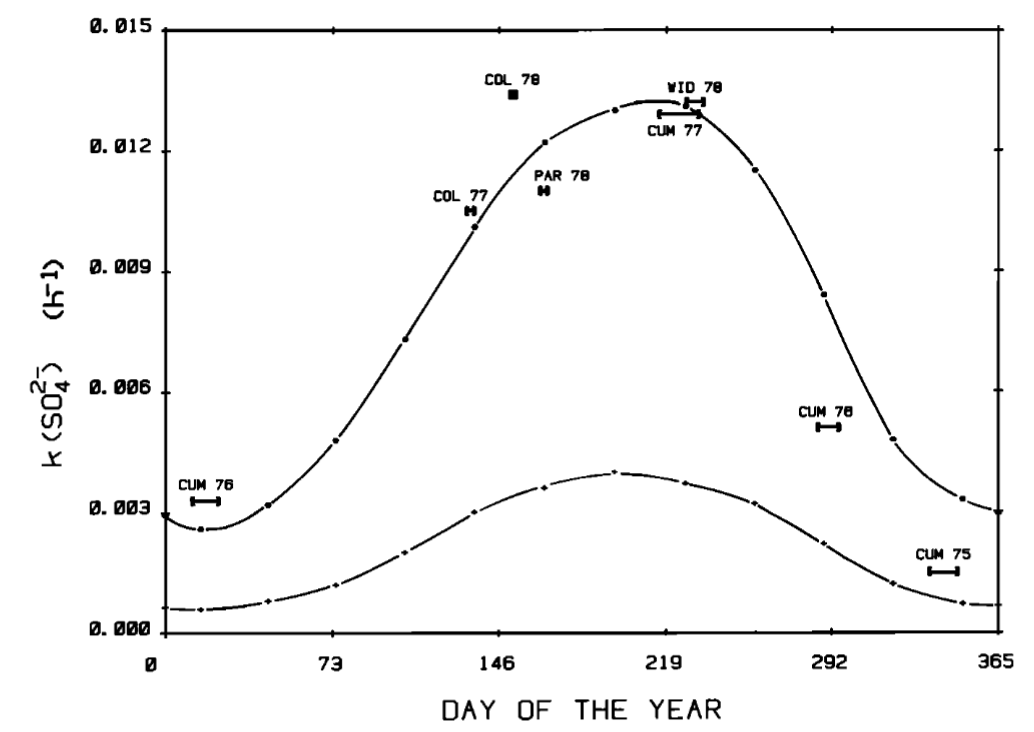
\includegraphics[width=0.8\linewidth]{Chapter4/Figs/meagher1983.png}
    \caption{Average rate of \ce{SO2} conversion to \ce{SO_4^{2-}} measured at different power station plumes. Also shown in this figure are the noontime (top curve) and diurnal average (bottom curve) \citep{meagherSeasonalVariationAtmospheric1983}}
    \label{fig:ch4:meagher1983}
\end{figure}


A field study by \citet{eatoughConversionSO2Sulfate1994} suggested that the aqueous-phase concentration of the oxidant and the reaction kinetics factors, including cloud droplet pH and temperature, were the two critical factors influencing the oxidation processes. \ce{SO2} dissolved into water droplets along with \ce{O3} and \ce{H2O2}. Both \ce{O3} and \ce{SO2} were moderately soluble in the pH range of 3--6, typical atmospheric acidity. Most of the dissolved \ce{SO2} were presented as \ce{HSO3^-} with the concentration of \qty{e-4}{M}. The atmospheric mixing ratio of tropospheric \ce{O3} generally fell in the range between 50-100 ppb, resulting in approximately \num[]{e-9} M. \ce{H2O2} was highly soluble, with the atmospheric mixing ratio between 0.1-5 ppb, aqueous concentration was expected at about \qty{e-4}{M} \cite{eatoughConversionSO2Sulfate1994}.

Another modelling study by \citet{feichterSimulationTroposphericSulfur1996} demonstrated the seasonal cycle of \ce{SO2} oxidation using ECHAM3, a more complex chemical scheme. The general circulation model (GCM) ECHAM3 developed at the Max-Planck Institute for Meteorology treated DMS and \ce{SO2} as gas and \ce{SO4^2-} as aerosol, all of which were prognostic variables. Emission, transport, chemistry and rainout of the sulfur species DMS, \ce{SO2} and sulfate were calculated online with the meteorology. The model offered a high temporal resolution but featured a coarse spatial resolution, which was insufficient to resolve synoptic-scale weather patterns adequately. Figure \ref{fig:ch4:feichter1996} shows the seasonal variation in \ce{SO2} oxidation and deposition. About half of sulfate aerosols formed in clouds during summer; the other half was a homogeneous gas-phase reaction. In winter, at least 90\% of sulfate aerosol was produced in the aqueous phase.


\begin{figure}
    \centering
    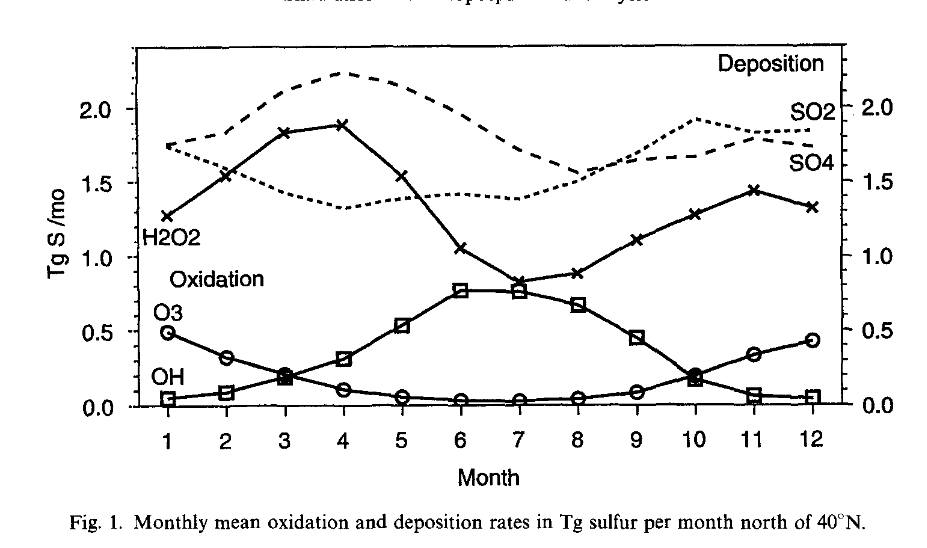
\includegraphics[width=0.8\linewidth]{Chapter4/Figs/feitcher1996.png}
    \caption{Monthly mean \ce{SO2} oxidation and deposition from ECHAM3 \citep{feichterSimulationTroposphericSulfur1996}}
    \label{fig:ch4:feichter1996}
\end{figure}


Recently, the seasonal difference of ERF due to aerosols was quantified \citep{bellouinRegionalSeasonalRadiative2016}. Four models participated in this simulation, including three general circulation models: ECHAM6-HAM2, HadGEM3-GLOMAP, NorESM1-M and one chemical transport model: OsloCTM2 \info{Based on the data portal, ECHAM6-1-05-LR, HadGEM2-A/AO/CC/ES, NorESM1-M participated in CMIP5}. In this study, simulations were run for one year after spin-up. Emissions from four regions (Europe, East Asia, the rest of the world, and the shipping sector) for the year 2008 were reduced by 20\%  to represent feasible emission reduction in two seasons: summer (May--October) and winter (November--April). In case of \ce{SO2} emissions, the perturbations reduced \ce{SO2} emissions by \num{-1.54} and \qty{-1.7}{Tg(S)~yr^{-1}} in Europe, \num{-6.28} and \qty{-6.7}{Tg(S)~yr^{-1}} in East Asia, and \num{-10.2} and \qty{-10.4}{Tg(S)~yr^{-1}} for the rest of the world, in summer and winter, respectively.

Emission rates were used to normalise each of the forcing's climate impacts to allow for comparison between emission rates, called the specific RF, as shown in Figure \ref{fig:ch4:bellouin2016}. HadGEM3-GLOMAP, which shared the same aerosol parameterisation as UKESM1, showed the largest change in ERF per unit of \ce{SO2} emissions in summer from Europe at \qty{-18}{(mW~m^{-2})~(Tg(\ce{SO2})~yr^{-1})^{-1}} or \qty{-0.036}{(W~m^{-2})~(Tg(S)~yr^{-1})^{-1}}.


\begin{figure}
    \centering
    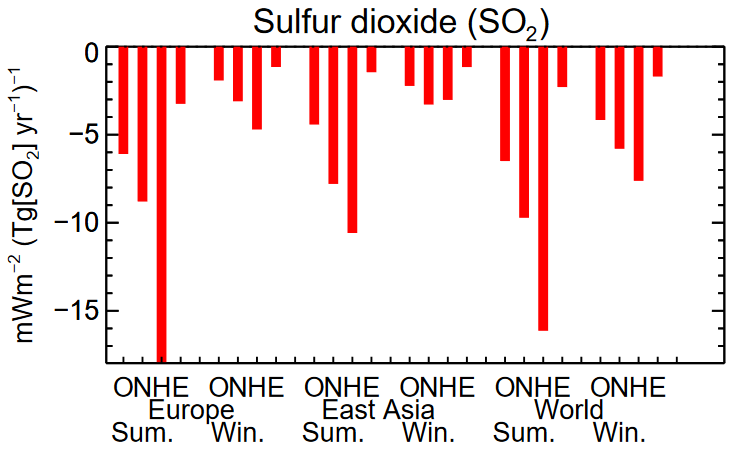
\includegraphics[width=0.5\linewidth]{Chapter4/Figs/bellouin2016.png}
    \caption[Specific radiative forcing (SRF) reported by \citet{bellouinRegionalSeasonalRadiative2016}]{ Specific radiative forcing (SRF) given in \unit{(mW~m^{-2})~(Tg(\ce{SO2})~yr^{-1})} for regional and seasonal reduction in \ce{SO2} emissions from four models:  OsloCTM2 (O), NorESM1-M (N), HadGEM3-GLOMAP (H) and ECHAM6-HAM2 (E) \citep{bellouinRegionalSeasonalRadiative2016}}
    \label{fig:ch4:bellouin2016}
\end{figure}

Despite extensive measurement campaigns in the late 20\textsuperscript{th} century to quantify the changes in \ce{SO2} and its oxidation and recent developments in the radiative effects of aerosols, no studies have shown quantitatively the link between seasonality of oxidation and the radiative impacts.

\subsection{Anomalous cooling in surface air temperature in CMIP6 models}
\label{ch4:sec:pothole}

Surface air temperature (TAS) is an indicator of climate change used to validate ESMs \citep[e.g. ][]{fanGlobalSurfaceAir2020,ipccClimateChange20132014}. All models participating in CMIP6 were required to provide \hist{} simulation, a coupled atmosphere-ocean simulation with historical emissions from 1850--2014, to be used to compare the model against each other and with observation \citep{eyringOverviewCoupledModel2016}. \citet{fanGlobalSurfaceAir2020} showed that models captured changes in surface air temperature in temporal evolution, especially between 1971 and 2014. The CMIP6 models, including UKESM1, underestimated TAS in high latitudes of the northern hemisphere from 1901 to 1970 but captured the seasonal variation in TAS from 1901 to 2014. 

In another study, six ESMs with interactive chemistry that participated in the CMIP6 and AerChemMIP, including UKESM1, were shown to exhibit a low bias in surface air temperature compared to observation between 1960 and 1989 \citep{zhangRoleAnthropogenicAerosols2021}. The anomalous cooling or the "pothole cooling" is the period between 1960 and 1989 inclusive when ESMs consistently underpredict the surface air temperature compared to observation \citep{zhangRoleAnthropogenicAerosols2021}. Figure \ref{fig:ch4:seasonal-tas-anomaly} shows the surface air anomaly from HadCRUT5 and UKESM1. HadCRUT5 is a gridded global historical surface temperature anomaly dataset relative to a 1961--1990 reference period. Data are available each month from January 1850 onwards on a 5-degree grid time series \citep{moriceUpdatedAssessmentSurface2021}. The TAS anomalies were readjusted for 1850--1859 climatology to show the evolution of temperature and pothole cooling. Annual mean surface temperature from UKESM1 agreed well with HadCRUT5 before and after the pothole period but showed especially cold bias in the Northern Hemisphere between 1960 and 1989. This behaviour was observed amongst other ESMs with varying degrees of bias but not in models with lower complexity. The cause for this behaviour is unclear \citep{zhangRoleAnthropogenicAerosols2021}.


\begin{figure}
    \centering
    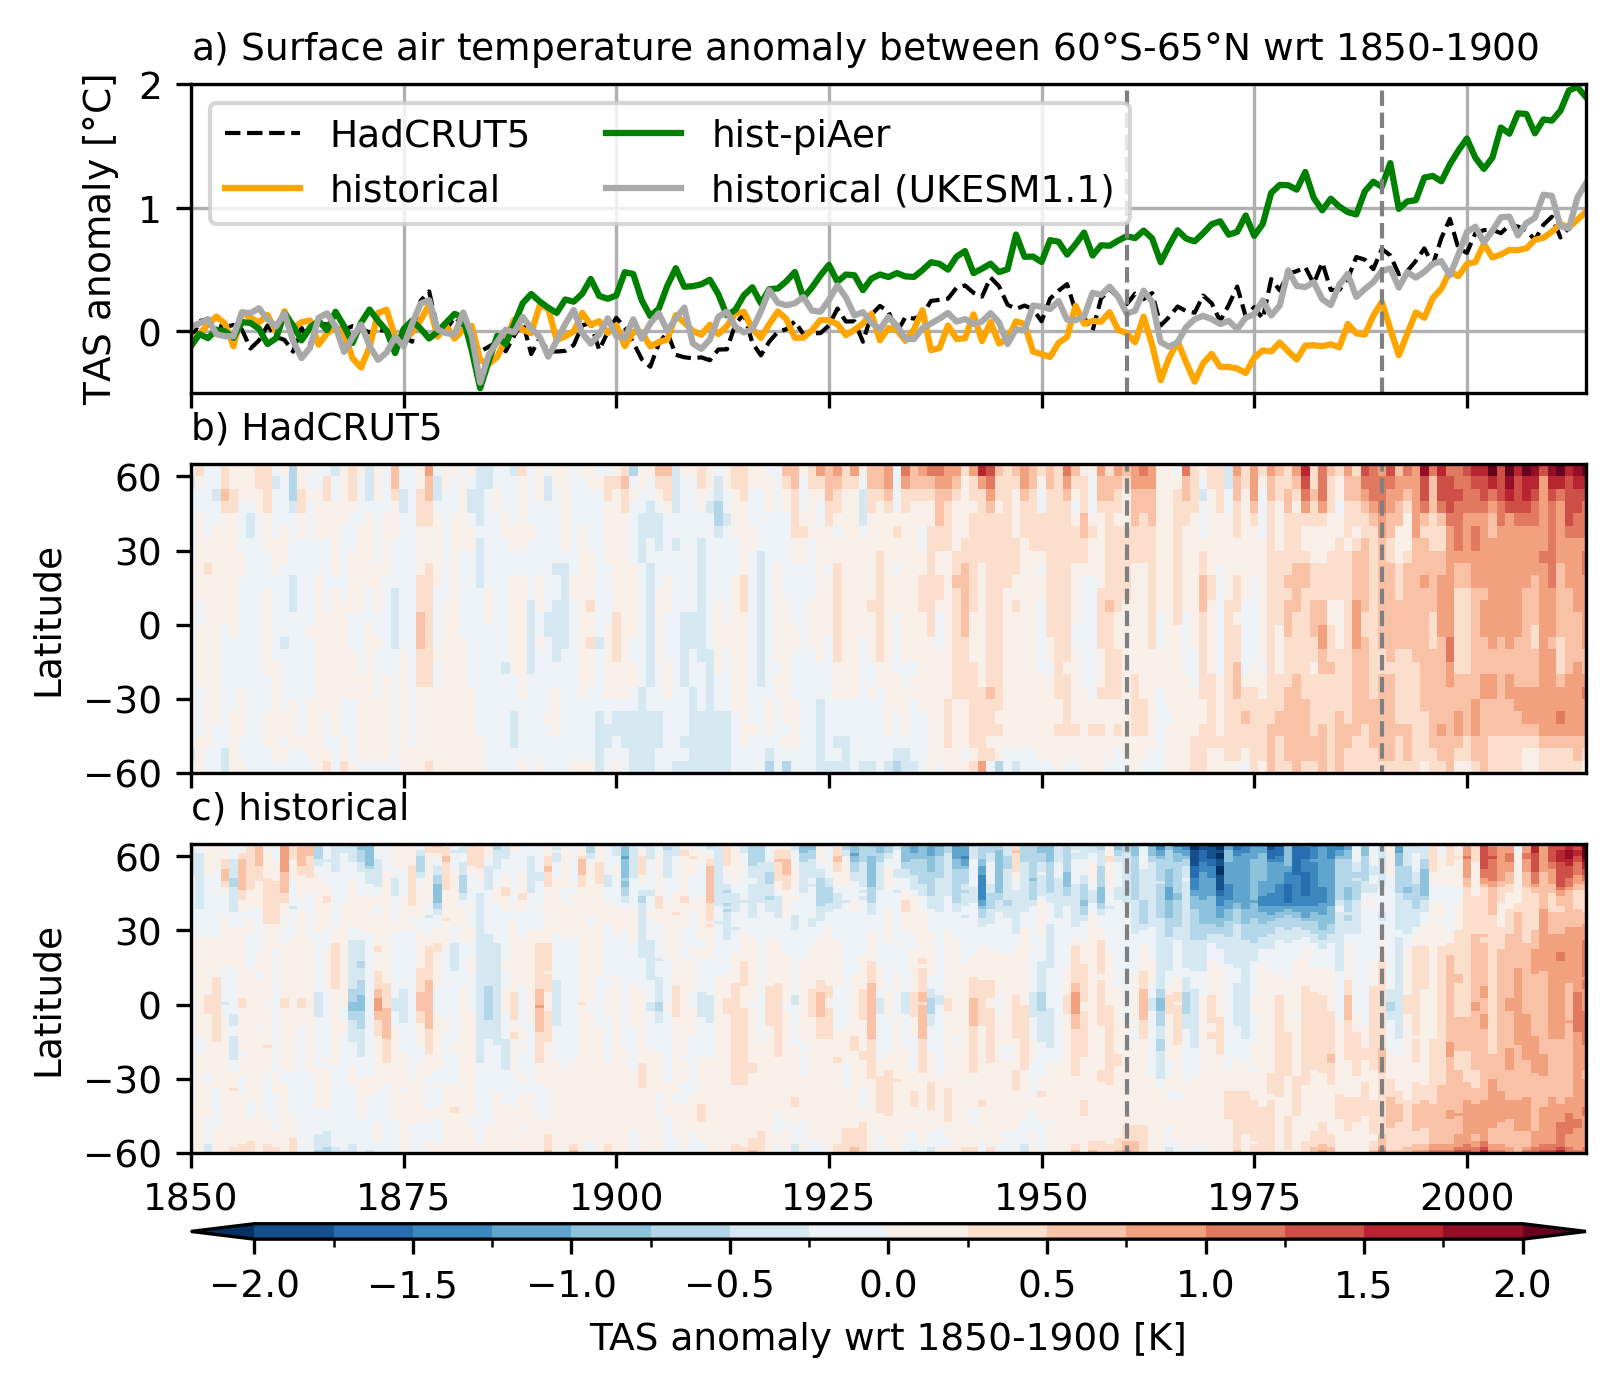
\includegraphics{Chapter4/Figs/TAS_anomaly_cropped.png}
    \caption[Surface air anomaly from HadCRUT5, UKESM1, and UKESM1.1 between 1850 and 2015]{a) Annual mean surface air temperature anomaly between 1850 and 2015 with respect to 1850 to 1859 averaged over latitude 60\textdegree S and 65\textdegree N. b) Surface air temperature anomaly from HadCRUT5 adjusted to 1850--1859. c) surface air temperature from UKESM1 \hist{} simulation. Grey dashed lines are the period between 1960 and 1989 when the ESMs consistently underpredict TAS and are called the pothole period.}
    \label{fig:ch4:seasonal-tas-anomaly}
\end{figure}


The large uncertainty in aerosol interaction and the resulting forcing on climate is due primarily to aerosol-cloud interactions and how the model represents these processes \citep{carslawLargeContributionNatural2013,ghanChallengesConstrainingAnthropogenic2016}. Thus, a better understanding of chemistry-aerosol-climate interaction is still needed to address the occurrence of pothole cooling.


\subsection{Research opportunities and motivation}

This chapter speculates that \ce{SO2} oxidised in summer and winter may lead to different radiative forcing. One could hypothesise that the aerosol-cloud interaction would be more substantial in the season with more gas-phase oxidation as gas-phase oxidation produces sulfuric acid that nucleates and forms new aerosol particles. While both measurement and modelling studies had confirmed the seasonal cycle of \ce{SO2} oxidation, there has not been a detailed modelling study of how this seasonal variation in aerosol formation would affect cloud formation in the historical period. 

UKESM1 simulates both aerosol mass and number independently, making it one of the most robust climate models regarding aerosol simulation. GLOMAP-mode, the aerosol scheme used in UKESM1, simulates sulfate aerosol using chemical production from gas and aqueous phases. It also simulates aerosol number and mass concentration independently with inter-modal interactions such as coagulation, condensation, and wet and dry deposition. This makes UKESM1 a valuable tool for studying the aerosol properties in different seasons.

A significant outcome of this chapter is how changes in seasonal oxidation may modulate the radiative effects of \ce{SO2} emissions with possible effects on the seasonal cycle of surface temperature anomaly. The following needs to be considered when considering the seasonal ERF: the annual cycle of oxidants, sulfate oxidation tendencies, aerosol and cloud properties. The seasonal cycle of ERF and the correlation between oxidation tendencies and aerosol properties are discussed, and changes in ERF per unit of \ce{SO2} emission are quantified. Lastly, this chapter discusses the correlation between observed seasonal variations in surface temperature anomaly, specifically during the pothole period, and the contribution to temperature changes from aerosols.


\section{Methods and data}

This chapter employs the AerChemMIP historical coupled atmosphere-ocean and fixed-SST transient simulation results from UKESM1. Both the model and simulation set-up are described in Chapter \ref{ch2:title}.

Atmosphere-ocean coupled simulations are used to attribute changes in surface air temperature to aerosol precursors. The control simulation, \hist{}, uses all historical emissions to drive the model. The perturbed simulation, \histpiaer{}, has aerosol precursor emissions set to the pre-industrial, i.e. 1850.

The experiment set up for calculating ERF is as follows. The control simulation, \textit{histSST}, uses prescribed historical SSTs from \hist{} with all historical emissions. The perturbed simulation, \textit{histSST-piAer}, also uses historical SST from \hist{} and has aerosol precursor emissions set to the pre-industrial (pi), i.e. 1850. In this chapter, \textit{histSST-piAer} is referred to as \sstpiaer{} for brevity.

A summary of simulations used in this chapter is given in Table \ref{ch4:tab:simulation}. The simulation configurations with all historical transient experiments from AerChemMIP that experiments cover the period between 1850 and 2014. "AOGCM" means atmosphere-ocean coupled simulation. "AGCM" means atmosphere-only simulation. "Hist" means the concentration or emission should evolve as for the CMIP historical simulation. "1850" means the concentrations or emissions should be fixed to the year 1850.

\begin{table}
   \caption[AerChemMIP experiments used in Chapter \ref{ch4:title}]{A summary of AerChemMIP experiments used in Chapter \ref{ch4:title}.}
   \label{ch4:tab:simulation}
   \centering
   \begin{tabular}{l c c}
    \toprule
     Experiment ID & Minimum model configuration & Aerosol precursors\\
    \midrule
     \textit{historical}      & AOGCM & Hist\\
     \textit{hist-piAer}      & AOGCM & 1850\\
     \textit{histSST}         & AGCM & Hist\\
     \textit{histSST-piAer} (abbrev. \sstpiaer{})  & AGCM & 1850\\
     \bottomrule
   \end{tabular}
\end{table}

\subsection{Seasonal cycle of \textsoo{} emissions}

Aerossol precursor emissions in AerChemMIP follow that of CEDS \citep{HoeslyHistoricalEmissions2017}. Aerosol precursors include not only \ce{SO2} but also organic carbon (OC) precursors and primary black carbon (BC) emissions. Using UKESM1 simulations for attribution experiments from AerChemMIP with 2014 emissions, \citet{oconnorAssessmentPreindustrialPresentday2021} showed that anthropogenic \ce{SO2} accounts for 79\% of total aerosol ERF. The ratio of \ce{SO2} emission to the total emission only decreases from 1950 \citep{hoeslyHistorical175020142018}, so it is possible to assume that \ce{SO2} is the main aerosol precursor outside of 2014. This chapter focuses on \ce{SO2} because it is the primary source for aerosol radiative effects. \info{Total aerosol: -1.09, SO2: -1.37, BC: 0.37, OC:-0.22 W/m2} 

\begin{figure}
    \centering
    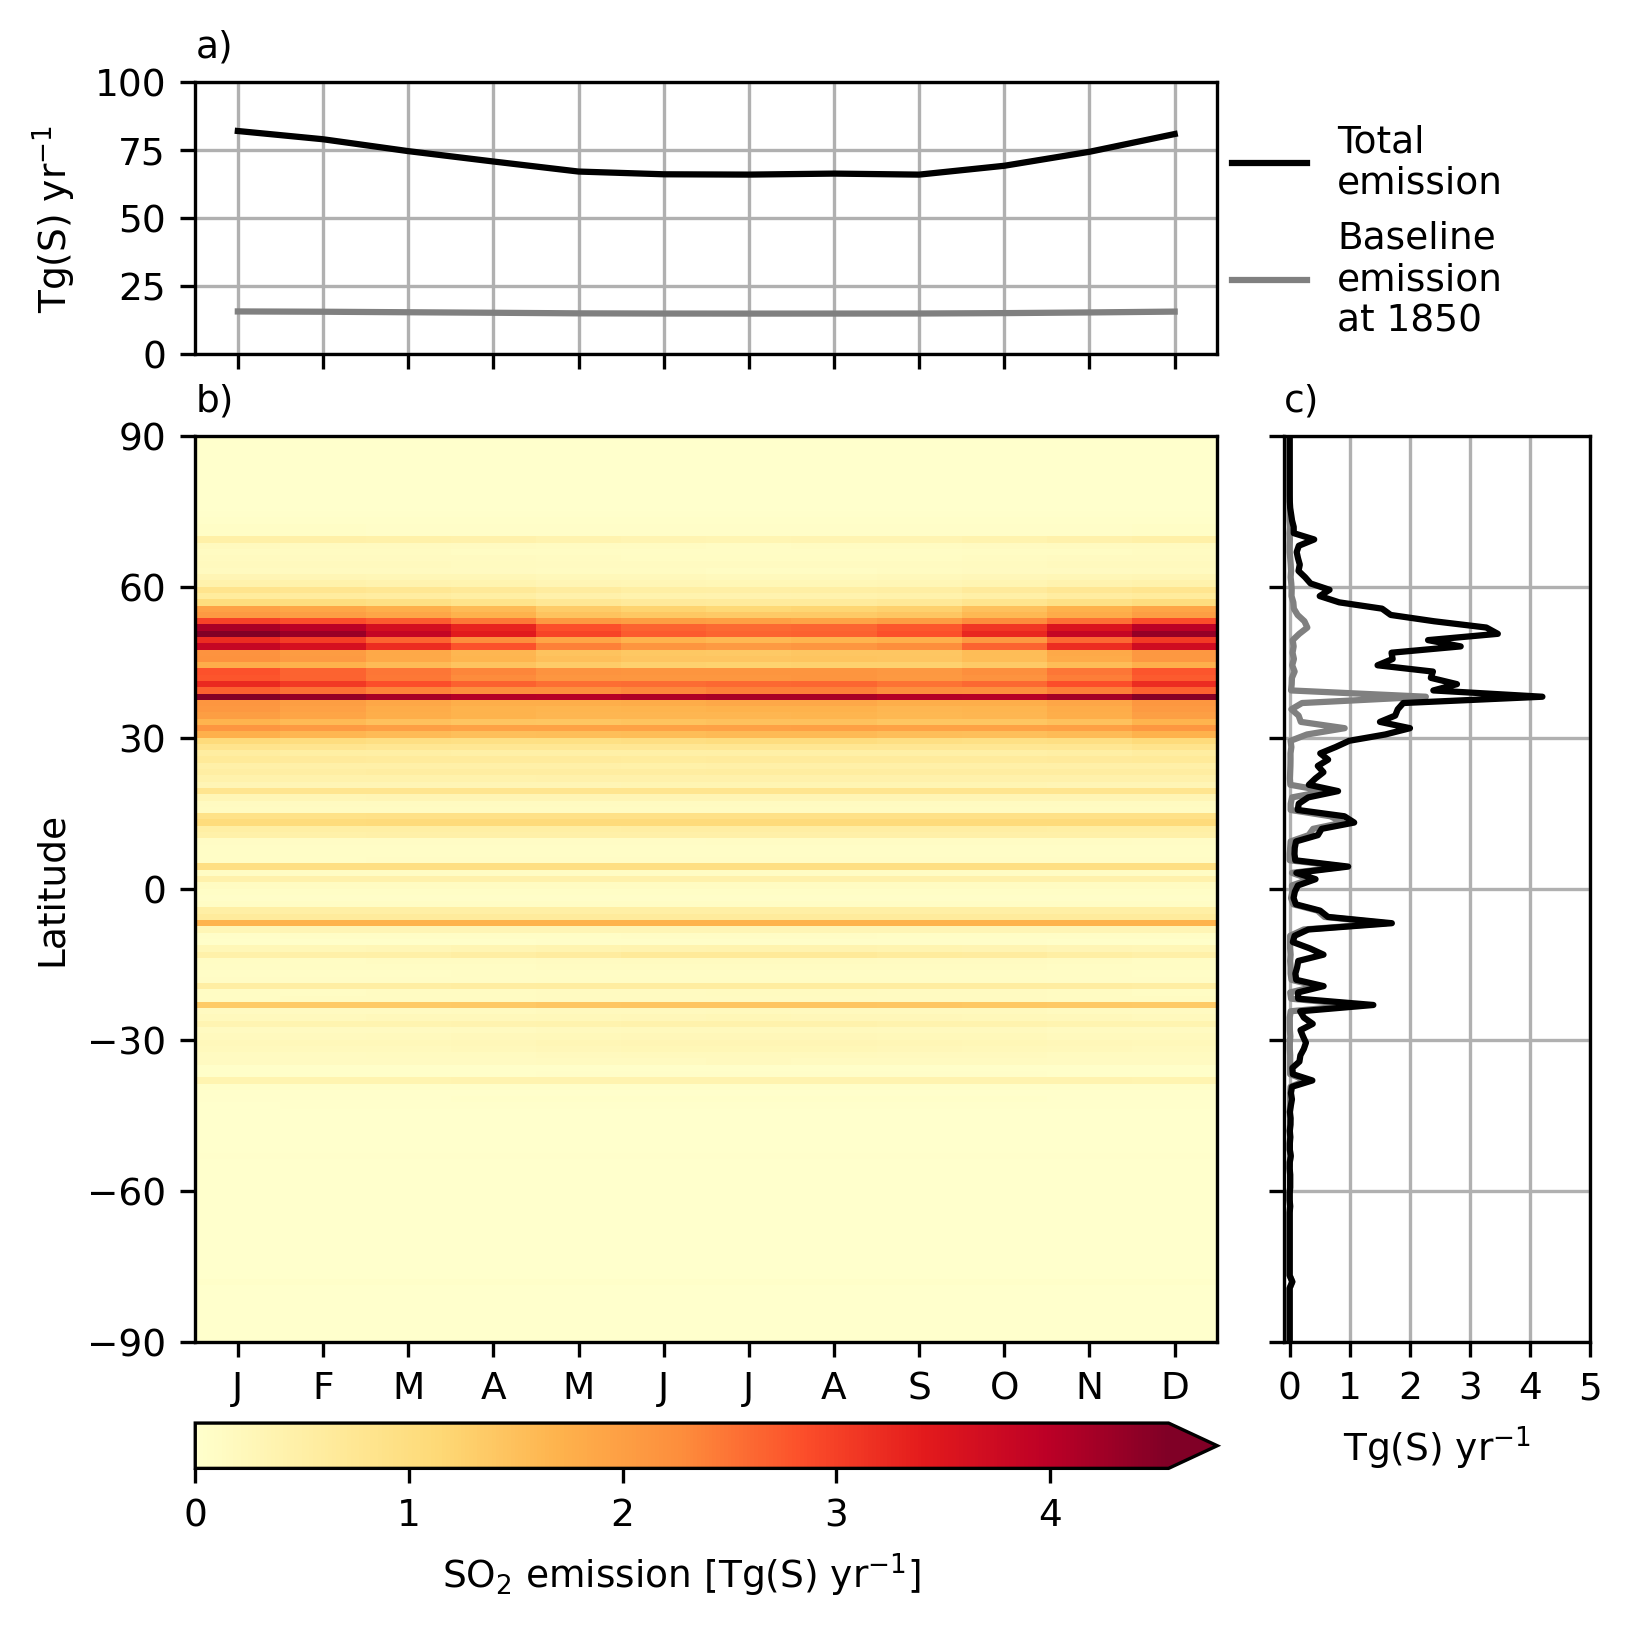
\includegraphics{Chapter4/Figs/emiso2_monthly_pothole.png}
    \caption[Primary \ce{SO2} emissions between 1960 and 1989]{Primary \ce{SO2} emissions between 1960 and 1989. (a) and (c) show total \ce{SO2} emissions from anthropogenic and non-anthropogenic sources at each month and latitude, respectively. (b) shows total emission as a function of month of year and latitude. Baseline emissions are constant and include both anthropogenic and natural emissions.}
    \label{fig:ch4:seasonal-emission}
\end{figure}

\ce{SO2} is the precursor of sulfate aerosols. Figure \ref{fig:ch4:seasonal-emission} shows the annual cycle in total primary, including anthropogenic and natural, emissions of \ce{SO2} between 1960 and 1989. Emissions from Europe and North America account for 32.1\% (\qty{24.6}{Tg(S)~yr^{-1}}) of the global annual 76.6 \unit{Tg(S)~yr^{-1}} emissions. The anthropogenic emissions increase in the boreal winter as energy usage rises with winter emissions approximately 12.5 \unit{Tg(S)~yr^{-1}} greater than summer emissions. Natural emissions are from volcanic activities. Volcanic eruptions are sporadic, and volcanic degassing contributes to background emissions, which have been constant throughout the years. Secondary \ce{SO2} emissions from DMS products are not included in primary emissions but are included in the model. Secondary \ce{SO2} is not reported in UKESM1 runs for AerChemMIP simulations. A similar UKESM1 setup for AMIP simulation covering the period 1981--1998 reported secondary \ce{SO2} emission at \qty{16.69}{Tg(S)~yr^{-1}}, accounting for 19\% of total \ce{SO2} sources \citep{mulcahyDescriptionEvaluationAerosol2020}. As a result, it could be said that the main source of \ce{SO2} is anthropogenic.

\section{Results and discussions}

This chapter focuses on the historical attribution of seasonal variation and changes due to aerosol precursor emissions, primarily \ce{SO2}, using existing AerChemMIP experiments. A period between 1960 and 1989 inclusive has been identified for analysis in this chapter for its high \ce{SO2} emissions and relatively low BC and OC emissions from the main emitting regions: Europe and North America \citep{hoeslyHistorical175020142018}. This period also coincides with the anomalous cooling period between 1960 and 1989. Another period of interest is the near present (2005--2015) when \ce{SO2} emissions increase in East and South Asia regions. 


\subsection{Seasonal variation of oxidants}

The fate of \ce{SO2} is partly controlled by the availability of oxidants. OH, \ce{O3} and \ce{H2O2} form photochemically in the atmosphere and are involved in oxidising \ce{SO2} in the model. Figure \ref{fig:ch4:seasonal-oxidants} shows global mean oxidant concentrations below 5 km aggregated by months in \unit{cm^{-3}} to focus on chemical kinetics. Both global airmass-weighted mean and latitudinal variation are shown. All oxidants' concentrations strongly correlate to insolation, where maximum concentration follows the solar radiation peaks. \ce{SO2} concentration localises near emission sources between latitude 30 and 60 \textdegree N and peaks in winter when emissions are more substantial, as shown in Figure \ref{fig:ch4:seasonal-emission}.

\begin{figure}
    \centering
    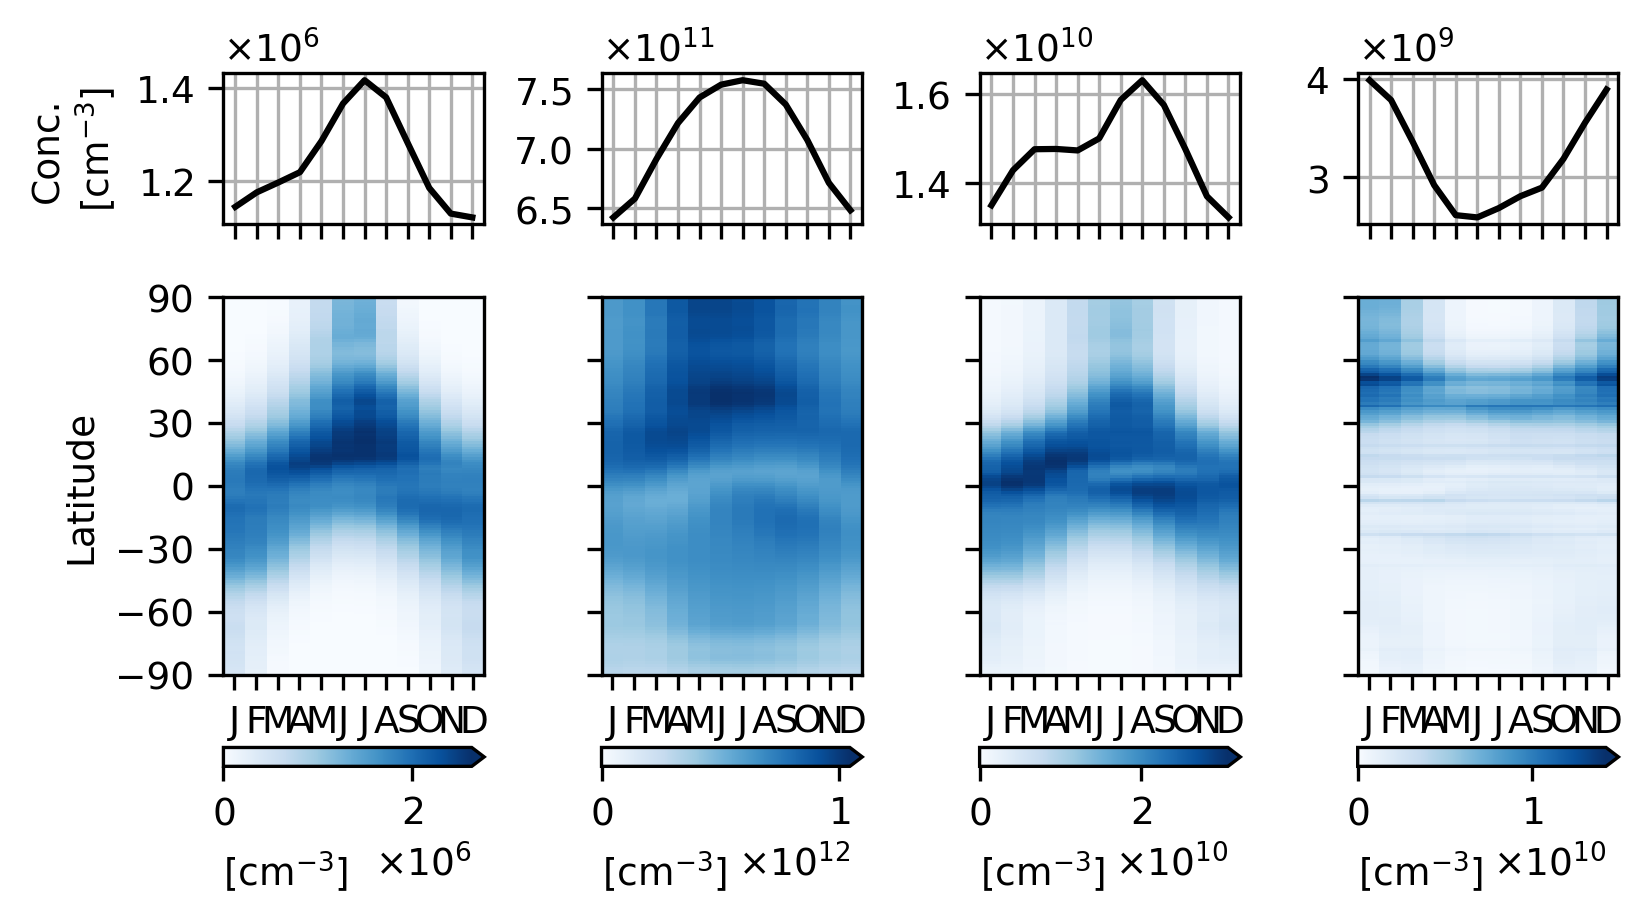
\includegraphics{Chapter4/Figs/seasonal_oxidant_pothole.png}
    \caption[Mean concentration of \ce{OH}, \ce{O3}, \ce{H2O2}, and \ce{SO2} from surface to 5 km between 1960 and 1989]{Global mean airmass-weighted concentration of (a) \ce{OH}, (b) \ce{O3}, (c), \ce{H2O2}, and (d) \ce{SO2} from surface to 5 km between 1960 and 1989 as a function of month of year. (e-g) show the respective oxidant concentration as a function of month of year and latitude for the same domain.}
    \label{fig:ch4:seasonal-oxidants}
\end{figure}

Between latitude 30 and 60 \textdegree N where most anthropogenic \ce{SO2} are emitted, OH and \ce{H2O2} concentrations vary greatly between seasons, with their summer concentrations one and two orders of magnitude greater than their respective winter concentrations. OH concentration increases from \num{2.4e5} to \qty{2.1e6}{\per\cubic\cm} and \ce{H2O2} concentration increases from \num{3.0e8} to \qty{2.3e10}{\per\cubic\cm}, as shown in Figure \ref{fig:app1:seasonal-oxidant-30-60}). 

While \ce{O3} concentration between latitude 30 and 60 \textdegree N is also greatest in the boreal summer months, exceeding \qty{1.1e12}{\per\cubic\cm}, its variation is not as drastic, with winter concentration over the same latitude band approximately half that of summer (\qty{7.2e11}{\per\cubic\cm}).

% Discuss SO2 loss via reaction with all the oxidants and refer to the emission seasonal cycle
\ce{SO2} concentration mimics its emission, reaching maximum in winter and minimum in summer. In summer, less \ce{SO2} is emitted, and more is oxidised, leading to a lower concentration and shorter lifetime in summer, discussed in the following section.

\subsection{Seasonal variation of oxidation}

\begin{figure}
    \centering
    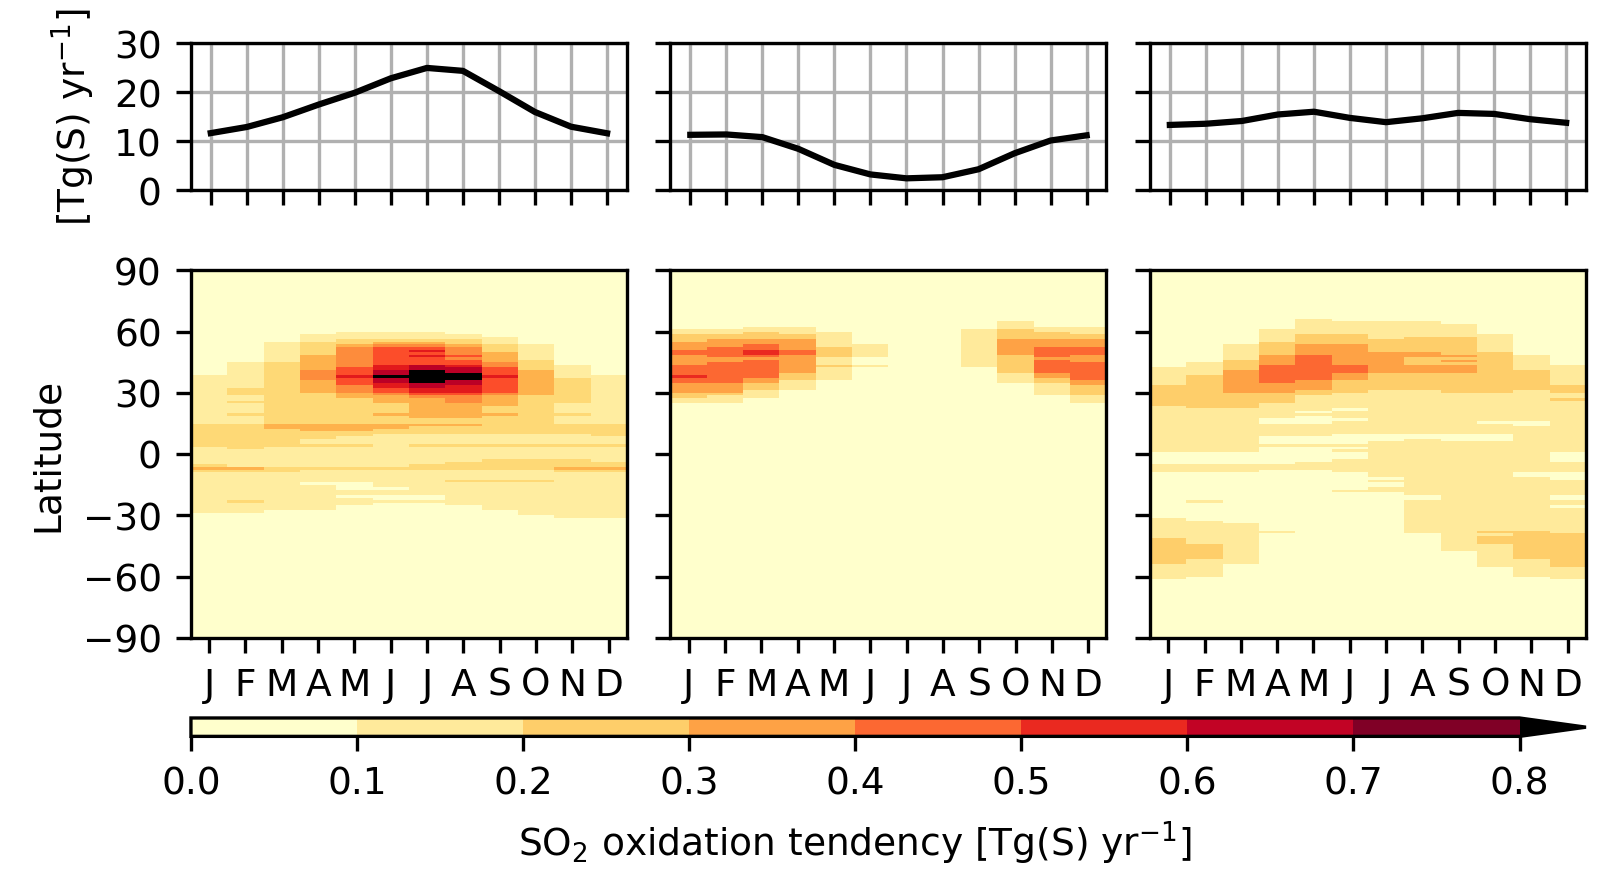
\includegraphics{Chapter4/Figs/seasonal_oxidation_w_summary_histsst_pothole.png}
    \caption[Total tropospheric \ce{SO2} oxidation tendencies as a function of latitude and months between 1960 and 1989]{Total \ce{SO2} oxidation with (a) OH, (b) \ce{O3}, and (c) \ce{H2O2} as a function of months between 1960 and 1989. (d-f) show the respective oxidation tendencies as a function of months and latitude for the same domain.}
    \label{fig:ch4:seasonal-oxidation}
\end{figure}

In the UKESM1, chemical reactions are the primary source of sulfate aerosols. \ce{SO2} reacts with OH in the gas-phase and with \ce{O3} and \ce{H2O2} in aqueous-phase inside cloud droplets. These pathways are controlled by different parameters, with the aqueous-phase reactions requiring the presence of clouds. Figure \ref{fig:ch4:seasonal-oxidation} shows the seasonal cycle in relevant gas- and aqueous-phase reactions aggregated by latitude. It can be seen that \ce{SO2 + OH} is maximal during boreal summer with an oxidation tendency reaching 25 \unit{Tg(S)~yr^{-1}}. This is expected as OH concentration is maximal during the same period in concurrence with the NH mid-latitude \ce{SO2} emissions. In contrast, the aqueous-phase reaction tendencies, \ce{SO2 + O3} and \ce{SO2 + H2O2}, do not follow the variations of their respective oxidants. This implies that the concentration levels of \ce{O3} and \ce{H2O2} are not the limiting factor for aqueous-phase oxidation in summer.  

The rate of oxidation may be limited in several ways. The seasonal cycle in \ce{SO2 + OH} would reflect the availability of both \ce{SO2} and OH while \ce{SO2 + O3} and \ce{SO2 + H2O2} do not. Both \ce{SO2 + O3} and \ce{SO2 + H2O2} take place in cloud droplets and are parameterised in UKESM1 using Equation \ref{ch4:eq:in-cloud-sulfate-prod} as discussed in Chapter \ref{ch2:title}. First, the gaseous oxidants dissolve into cloud droplets. This process is limited by the oxidants' concentrations and their Henry's coefficients, which control the solubility of gases. The dissolved oxidants react according to reaction rates that depend on the cloud droplet's temperature, pressure, and pH. This way, the amount of cloud droplets controls the sulfate production rate as it determines the amount of available water in each model grid.

% Define cf and lwc
Cloud properties, including cloud fraction and liquid water path, are crucial parameters in aqueous-phase reactions. Cloud processes are parameterised to simulate clouds in Earth System models with coarse grids. Cloud fraction, sometimes referred to as cloud cover, is a parameter which represents the fraction of the total volume of the model grid box that contains any cloud. It is unitless with a value between zero and one. Cloud liquid water content describes the mass of liquid water in a unit volume of air and has the unit of \unit{\gram\per\cubic\metre}.

\begin{figure}
    \centering
    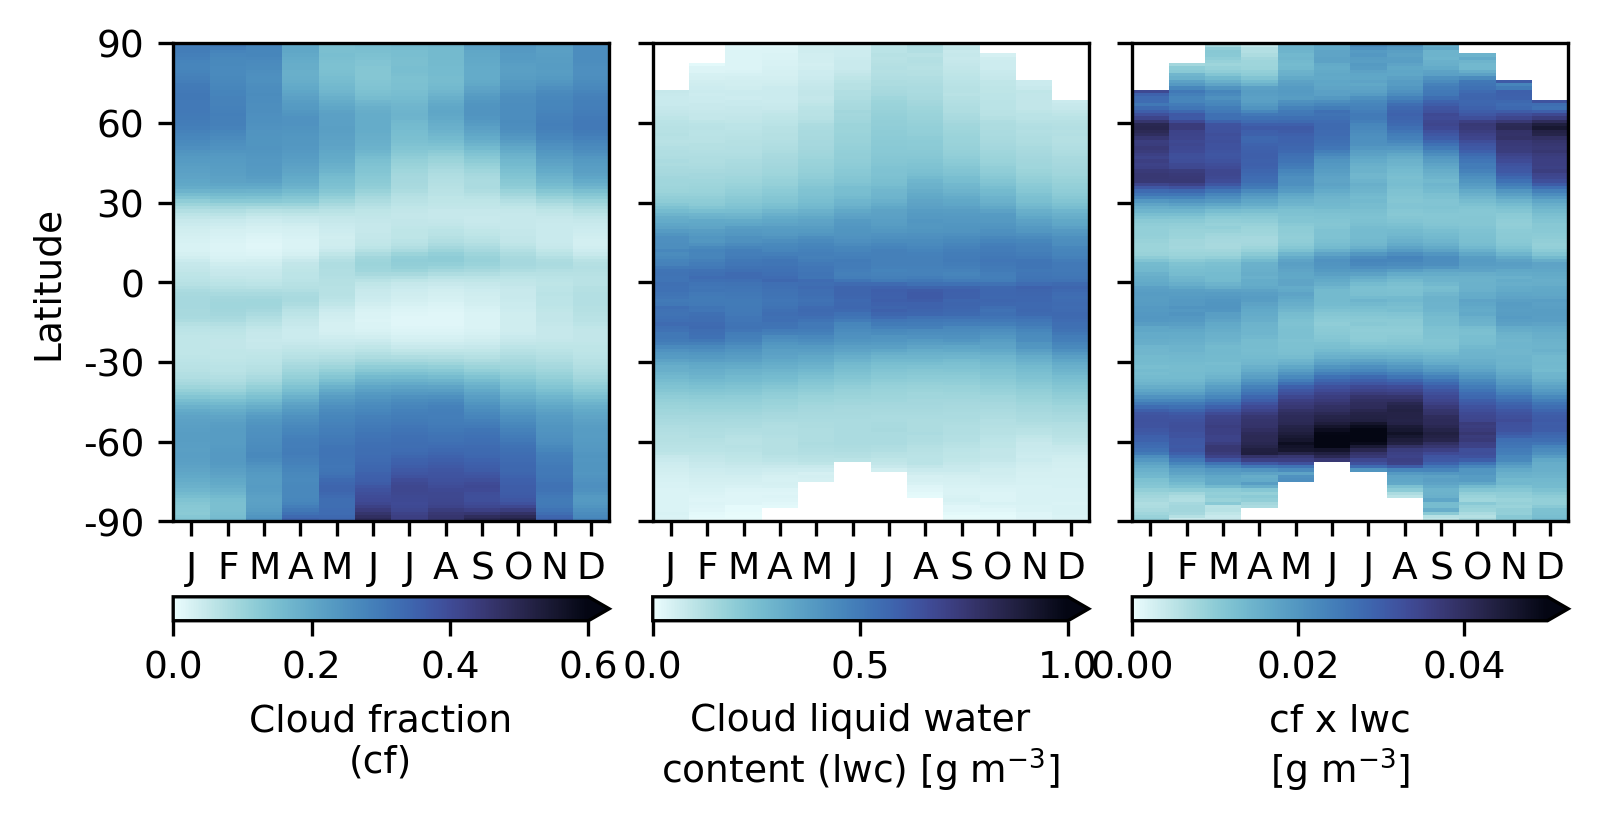
\includegraphics{Chapter4/Figs/seasonal_cf_lwc_histsst_pothole.png}
    \caption[Mean cloud fraction and liquid water content below 10 km between 1960 and 1989]{Mean (a) cloud fraction, (b) liquid water content and (c) products of cloud fraction and liquid water content as a function of latitude and month of the year from the surface up to 10 km between 1960 and 1989.}
    \label{fig:ch4:seasonal-cf-lwc}
\end{figure}

Both cloud fraction and cloud liquid water content enable the dissolution of gaseous oxidants into cloud droplets. Figure \ref{fig:ch4:seasonal-cf-lwc} shows seasonal variations of both parameters and their products as a function of months and latitude. Higher cloud fraction collocates with lower liquid water content in the mid-latitudes. The products of cloud fraction and liquid water content are greater than \qty{0.03}{\gram\per\cubic\metre} except for summer for mid-latitude, which explains the lower aqueous-phase reaction during the same season. 

As explored in section \ref{ch2:sec:so4-prod-rate}, aqueous-phase production by \ce{O3} and \ce{H2O2} increases by two orders of magnitudes in winter compared to summer conditions, placing \ce{SO2 + O3} in the same order of magnitude of \ce{SO2 + OH}. This increase in aqueous-phase production in winter comes from more significant cloud fractions. 

It can be seen that the relationship between cloud fraction and aqueous-phase production rate explains the seasonal variations observed in Figure \ref{fig:ch4:seasonal-oxidation}. These results illustrate that cloud is integral to aerosol-cloud-climate interaction in UKESM1 and other ESMs. 


\subsection{Drivers of sulfur loss budget terms}
\label{ch4:sec:sulfur-loss}

Oxidation is not the only process that influences the amount of aerosol in the atmosphere. \ce{SO2} may be removed by deposition before it is oxidised into sulfate. Once oxidised, sulfate also undergoes deposition, removing it from the atmosphere. All loss processes play a part in determining the lifetime of both sulfur species. This section explores the importance of deposition in determining the sulfur budget and its variation throughout the year.

\begin{figure}
    \centering
    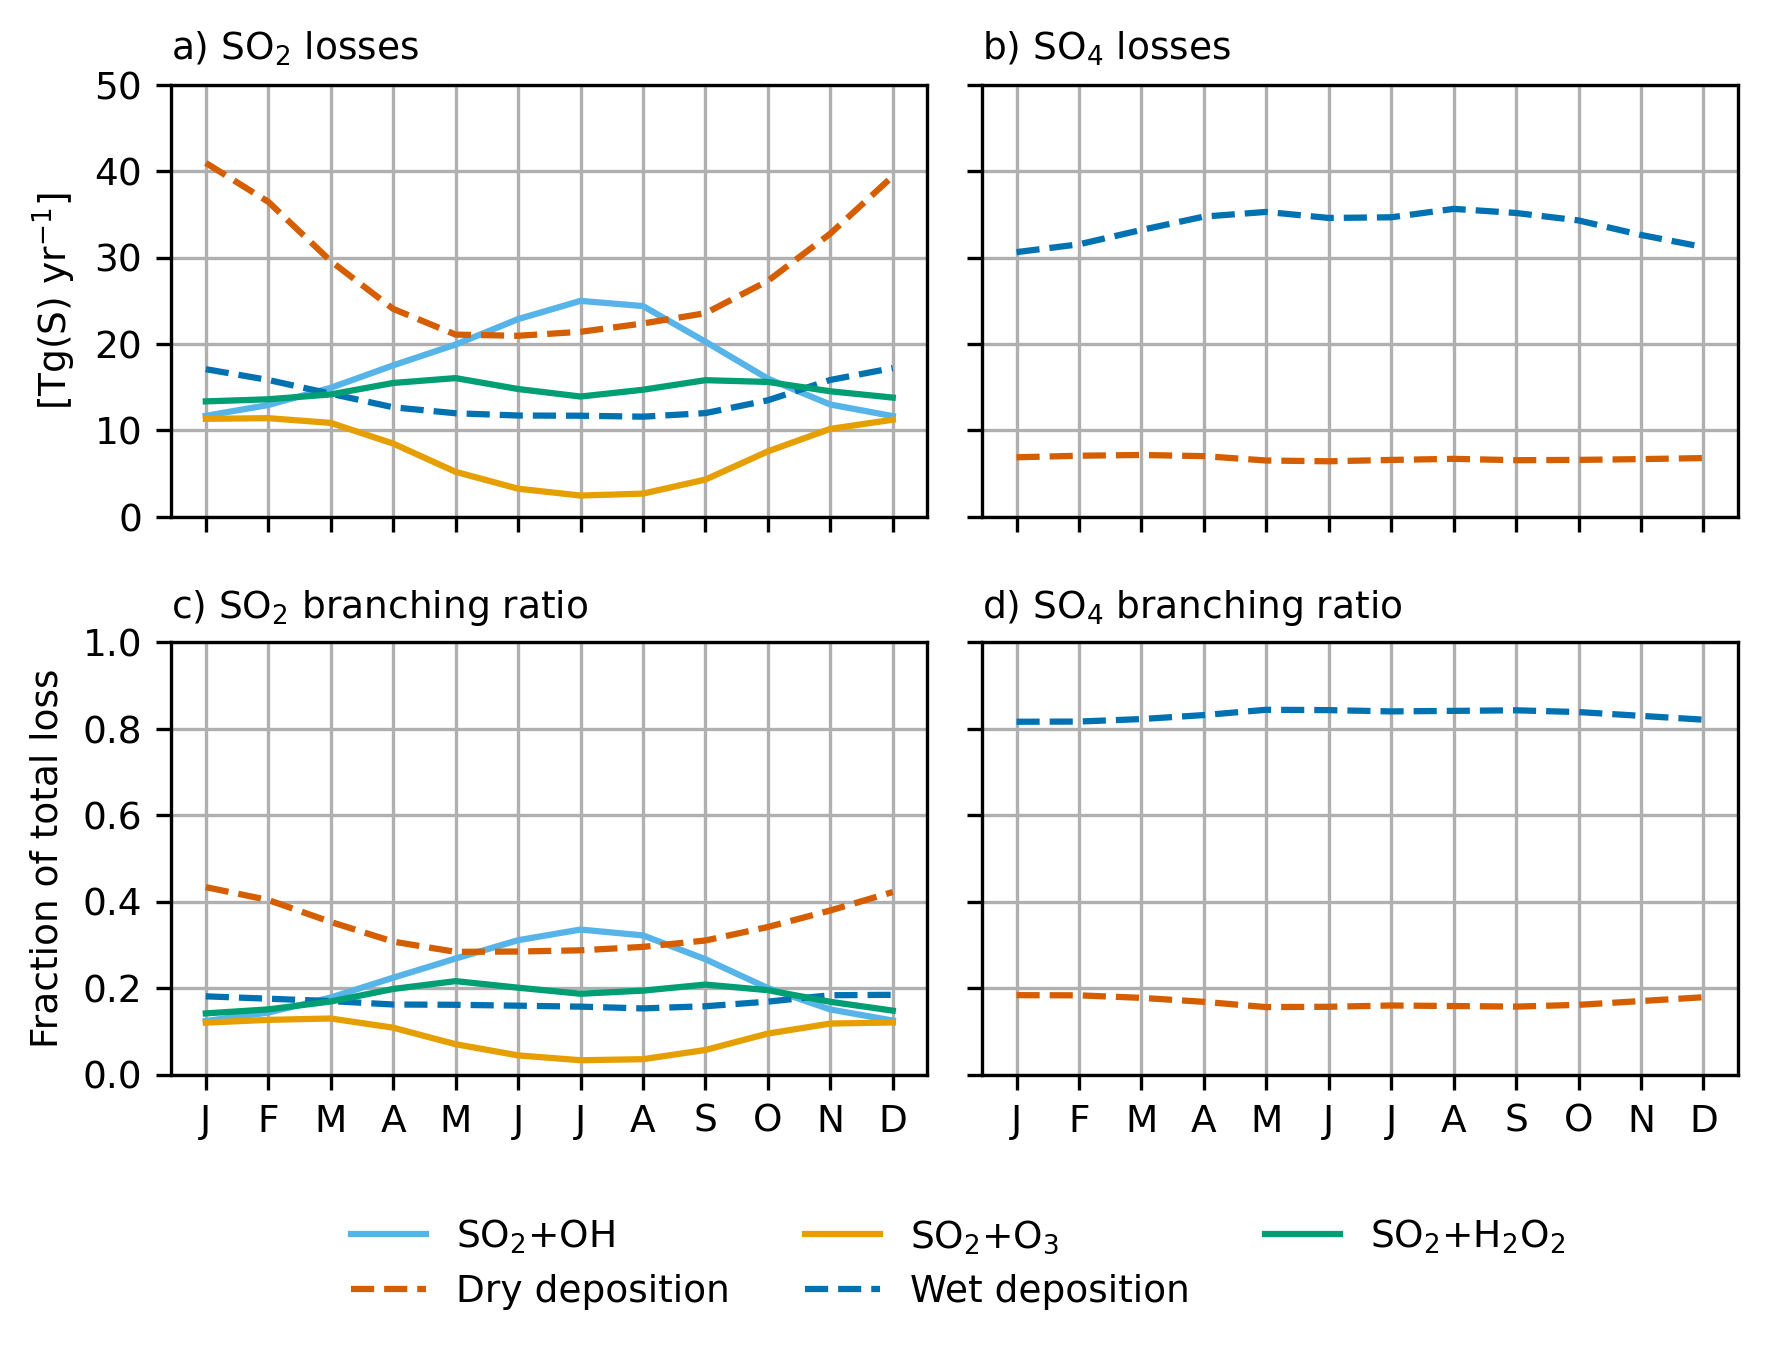
\includegraphics{Chapter4/Figs/branching_ratio_histsst_pothole.png}
    \caption[Absolute and relative losses for \ce{SO2} and \ce{SO4} by month of year between 1960 and 1989]{Absolute and relative losses for \ce{SO2} and \ce{SO4} by month of year between 1960 and 1989. (a-b) Total seasonal \ce{SO2} and \ce{SO4} loss tendency. (c-d) \ce{SO2} and \ce{SO4} loss tendency relative to total losses.}
    \label{fig:ch4:seasonal-branching-ratio}
\end{figure}

\ce{SO2} is lost through oxidation, wet and dry deposition. Figure \ref{fig:ch4:seasonal-branching-ratio} shows the loss tendencies of \ce{SO2} and sulfate aggregated by month. It can be seen that \ce{SO2} has a different fate depending on the emitted month. During the boreal summer months, 35\% of \ce{SO2} is oxidised by OH, surpassing dry deposition. \ce{SO2 + O3} shows large, but opposite trend to \ce{SO2 +OH}, seasonal variation, contributing less than 10\% in summer and reaching 15\% in winter. The wet deposition trend follows emissions, and the fraction of the total loss it contributes is largely constant at 18\%. As more \ce{SO2} oxidises and forms sulfate in summer, sulfate losses increase in the same season as there is more sulfate. The ratio between sulfate wet and dry deposition is relatively constant throughout the year.

\ce{SO2} losses in UKESM1 shares similar trends with previous work. Compared to monthly mean \ce{SO2} oxidation from ECHAM3 \citep{feichterSimulationTroposphericSulfur1996}, both models show a maximal \ce{SO2 + OH} tendency in summer and \ce{SO2 + O3} in winter. Gas-phase oxidation with OH during winter is minimal, with an annual mean in percentage of total loss of 17.2\% and 15\% for ECHAM3 and UKESM1, respectively. Ratios of annual mean \ce{SO2} oxidation with \ce{O3} in ECHAM3 and UKESM1 are 4.4 and 7\%, respectively. However, UKESM1 predicts \ce{SO2} oxidation with \ce{H2O2} to be 50\% less than that of ECHAM3 (30 compared to 19\%). The lower \ce{SO2 + H2O2} in UKESM1 is supplemented by higher wet deposition, leading to a similar lifetime of \ce{SO2} for both models. ECHAM3 and UKESM1 predict \ce{SO2} lifetime at 1.6 and 2.1 days, respectively (Figure \ref{fig:ch4:seasonal-s-lifetime}).

This section has attributed sulfate aerosol formation to gas- and aqueous-phase oxidation, which vary significantly throughout the year. Close to half of \ce{SO2} is removed by deposition. Gas-phase oxidation is the main oxidation pathway during summer. The following section looks at the impact of \ce{SO2} emissions during the pothole period compared to the 1850s.

\subsection{Attribution of \textsoo{} budget to \textsoo{} emission increase during pothole period}

Global \ce{SO2} emissions have quadrupled in 1960 compared to the 1850s (Section \ref{sec:ch3:emissions}). The abundance of \ce{SO2} may shift the limiting factor of chemical reaction from \ce{SO2} to the oxidants, having knock-on effects on the sulfur budget. This section describes the change in the sulfur budget compared to emissions in the 1850s to quantify the changes to the increased emissions. 

\begin{figure}
    \centering
    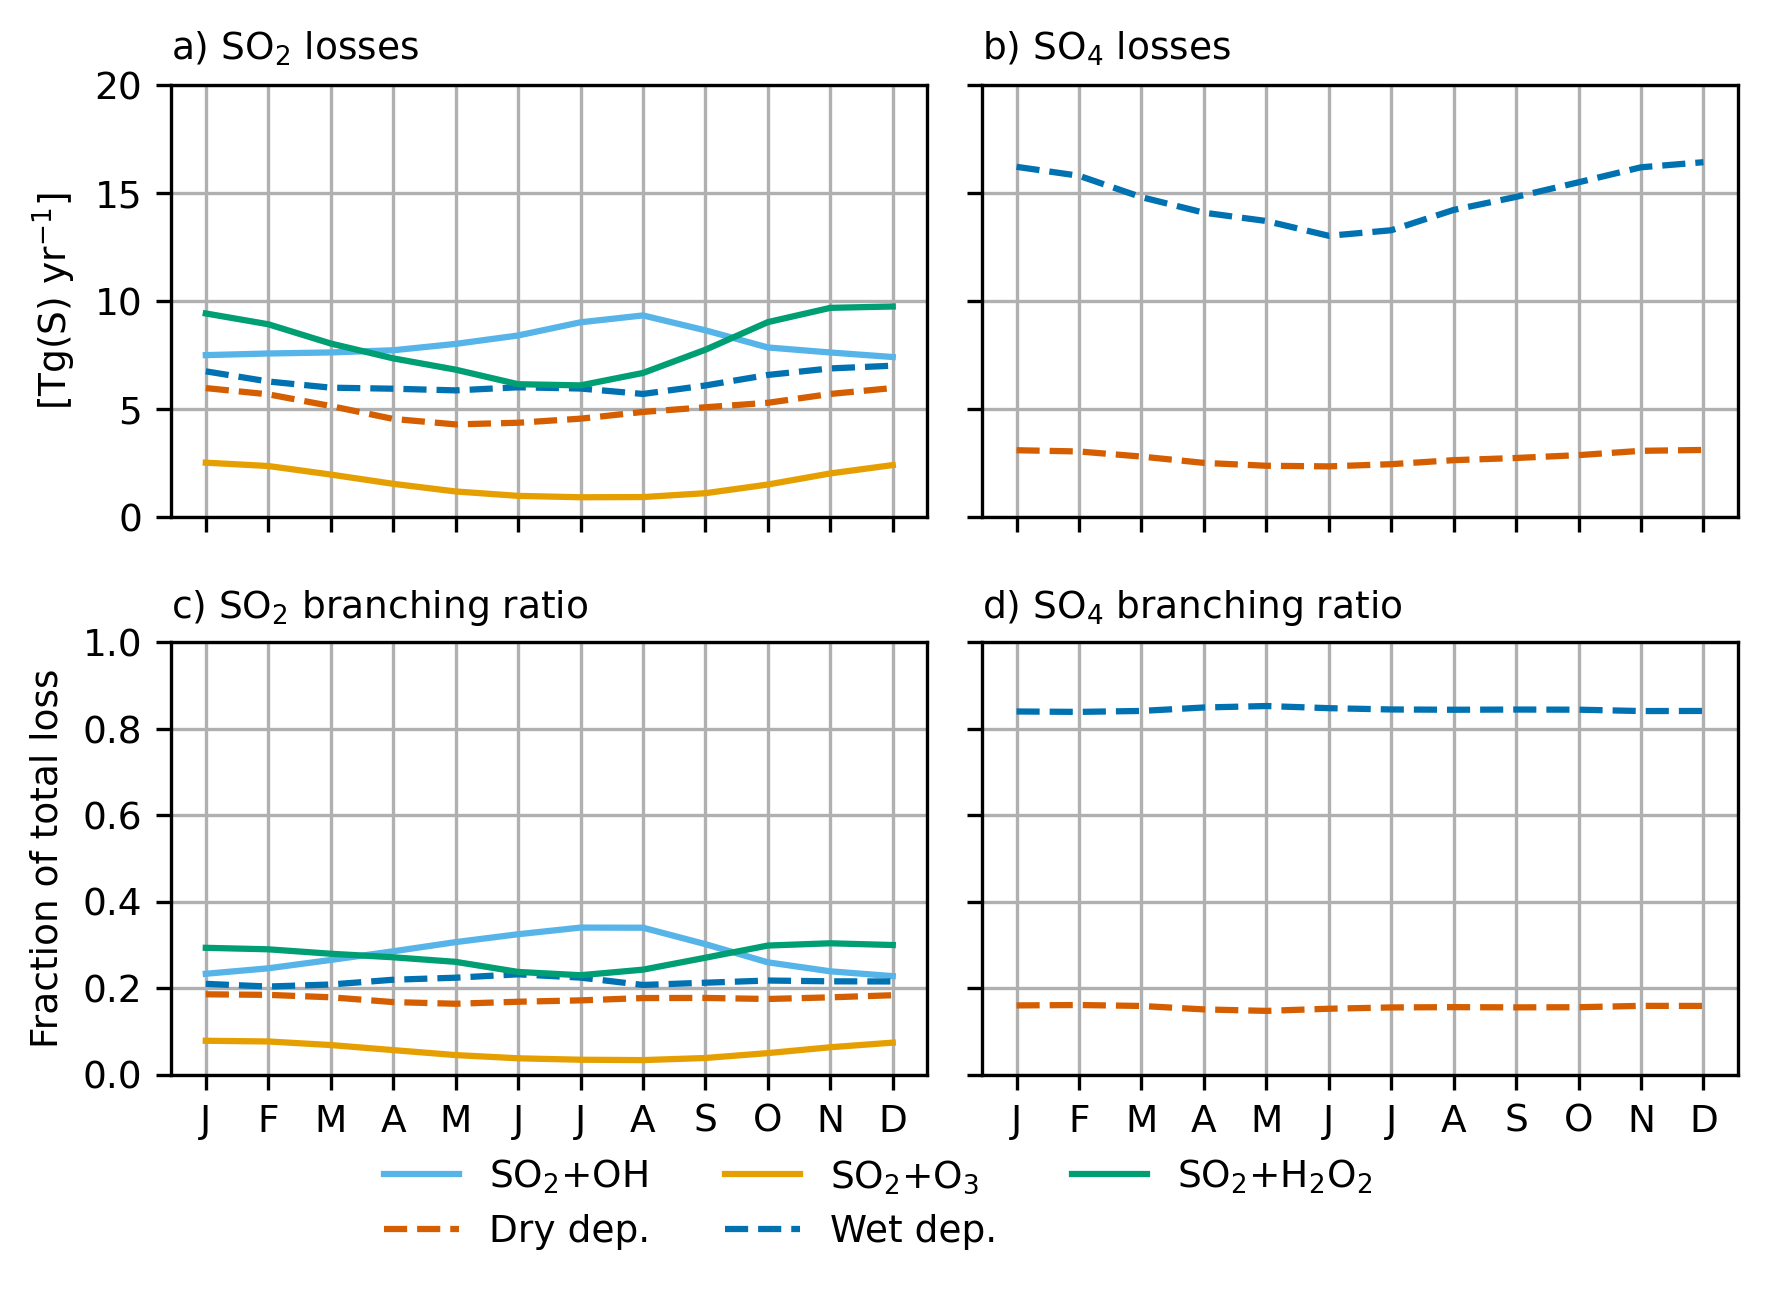
\includegraphics{Chapter4/Figs/branching_ratio_sstpiaer_pothole.png}
    \caption[Absolute and relative losses for \ce{SO2} and \ce{SO4} by month of year between 1960 and 1989 when aerosol precursor emissions are constrained at 1850 level (\sstpiaer{})]{Absolute and relative losses for \ce{SO2} and \ce{SO4} by month of year between 1960 and 1989 from \sstpiaer{}. (a-b) Total seasonal \ce{SO2} and \ce{SO4} loss tendency. (c-d) \ce{SO2} and \ce{SO4} loss tendency relative to total losses.}
    \label{fig:ch4:seasonal-branching-ratio-sstpiaer}
\end{figure}

To understand the seasonal variation in \ce{SO2} losses seen in section \ref{ch4:sec:sulfur-loss}, the seasonal variation of sulfur losses without the increase in \ce{SO2} emissions are quantified. Figure \ref{fig:ch4:seasonal-branching-ratio-sstpiaer} shows the seasonal cycle of absolute and relative losses for \ce{SO2} and sulfate during the pothole period while \ce{SO2} emissions are kept at the pre-industrial level (from \sstpiaer{}). \ce{SO2} oxidations vary with seasons without increased anthropogenic \ce{SO2} emissions. \ce{SO2} oxidation with \ce{H2O2} exhibits the largest change, with 10\% less oxidation, when \ce{SO2} emissions follow historical trajectory. The proportion of the loss to deposition has increased when \ce{SO2} emissions follow the historical trajectory, showing annual mean 20\% of loss is due to dry deposition in \sstpiaer{} compared to 35\% in \histsst{}. Moreover, \ce{SO2} emissions during the pothole period increase \ce{SO2} dry deposition by 12\% and 30\% in summer and winter. This implies the atmosphere may not have enough capability to oxidise all \ce{SO2} emitted in the 1980s, as shown by the larger proportion of \ce{SO2} deposited compared to a lower proportion of dry deposition when \ce{SO2} emissions are lower.

\begin{figure}
    \centering
    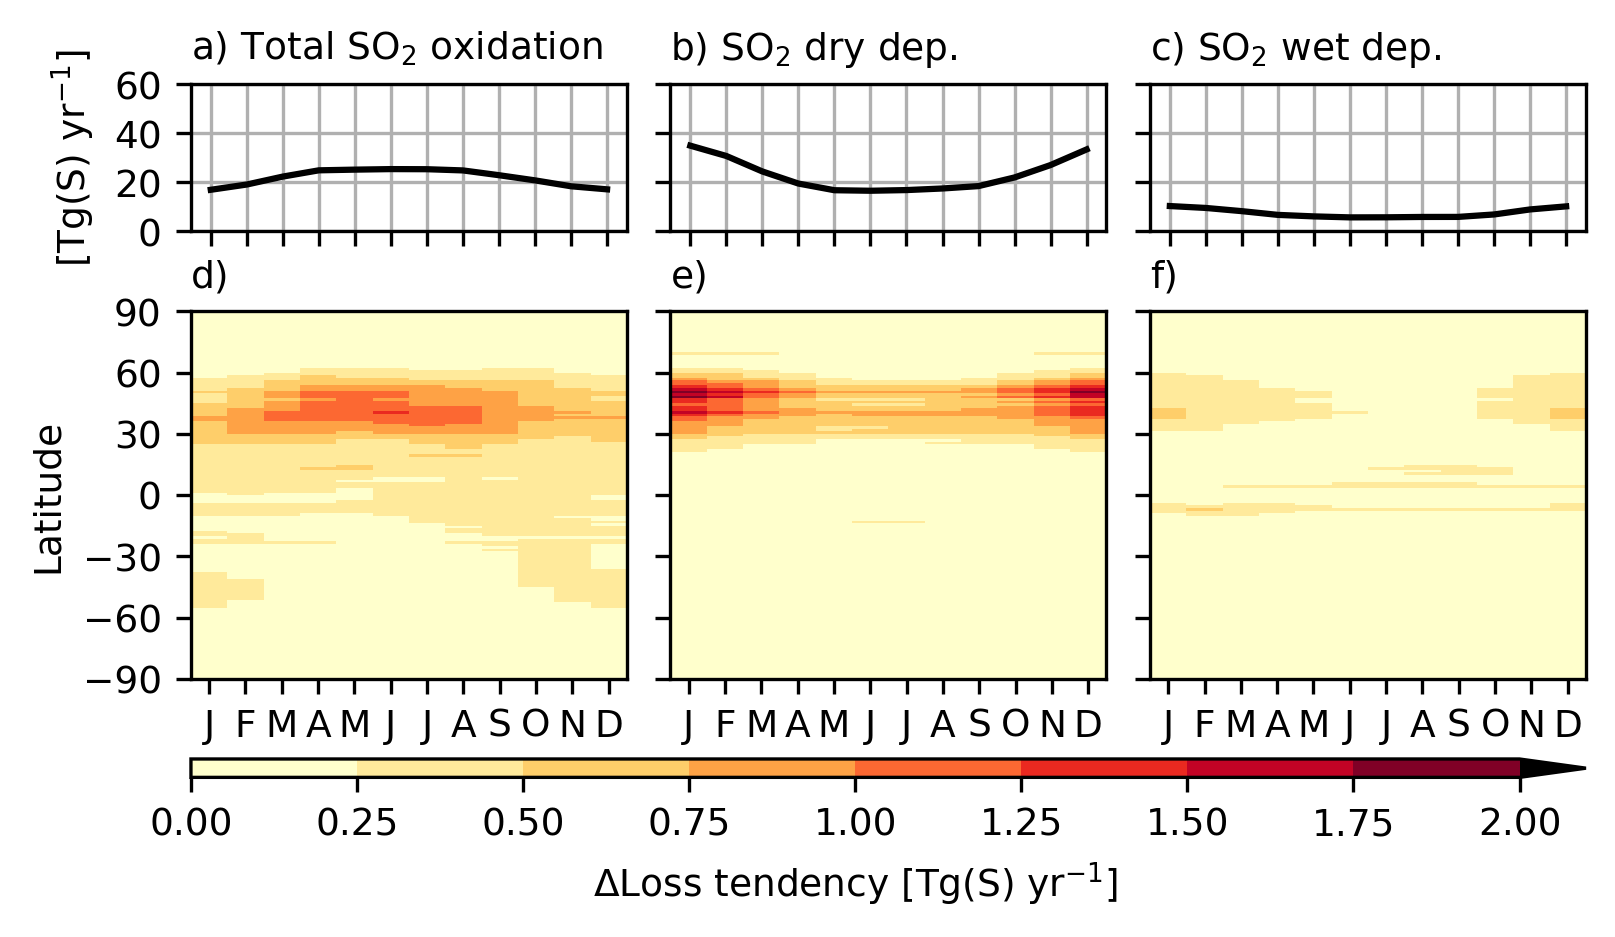
\includegraphics{Chapter4/Figs/so2_losses_histsst_pothole.png}
    \caption[\ce{SO2} loss tendencies due to oxidation and deposition by months between 1960 and 1989 due to aerosol precursor emissions]{\ce{SO2} loss tendencies due to oxidation and deposition by months 1960 and 1989. (a-c) Total seasonal \ce{SO2} loss tendency. (d-f) \ce{SO2} loss tendency as a function of month of year and latitude. This plot is a difference between \histsst{} and \sstpiaer}
    \label{fig:ch4:so2-loss}
\end{figure}

As the increased emissions between 1960 and 1989 reduced the ratio of \ce{SO2} being oxidised compared to total loss, it is also crucial to identify whether the increase in emission has changed the seasonal variation of each loss term and the location of the loss process. Figure \ref{fig:ch4:so2-loss} illustrates the change in \ce{SO2} losses due to aerosol precursor emissions (\histsst{} minus \sstpiaer{}). Dry deposition removes anthropogenic \ce{SO2} near emission sources along the latitude band between 30 and 60 \textdegree N. Dry deposition is more significant in boreal winter when there is more emission than in winter (40 \unit{Tg(S)~yr^{-1}} compared to 20 \unit{Tg(S)~yr^{-1}}). Wet deposition is the lowest of all loss processes, with an annual mean tendency of 10 \unit{Tg(S)~yr^{-1}} in January. Wet and dry deposition correlates with emission variations (high emissions in boreal winter), but oxidants and cloud properties explain the chemical production.


% \begin{figure}
%     \centering
%     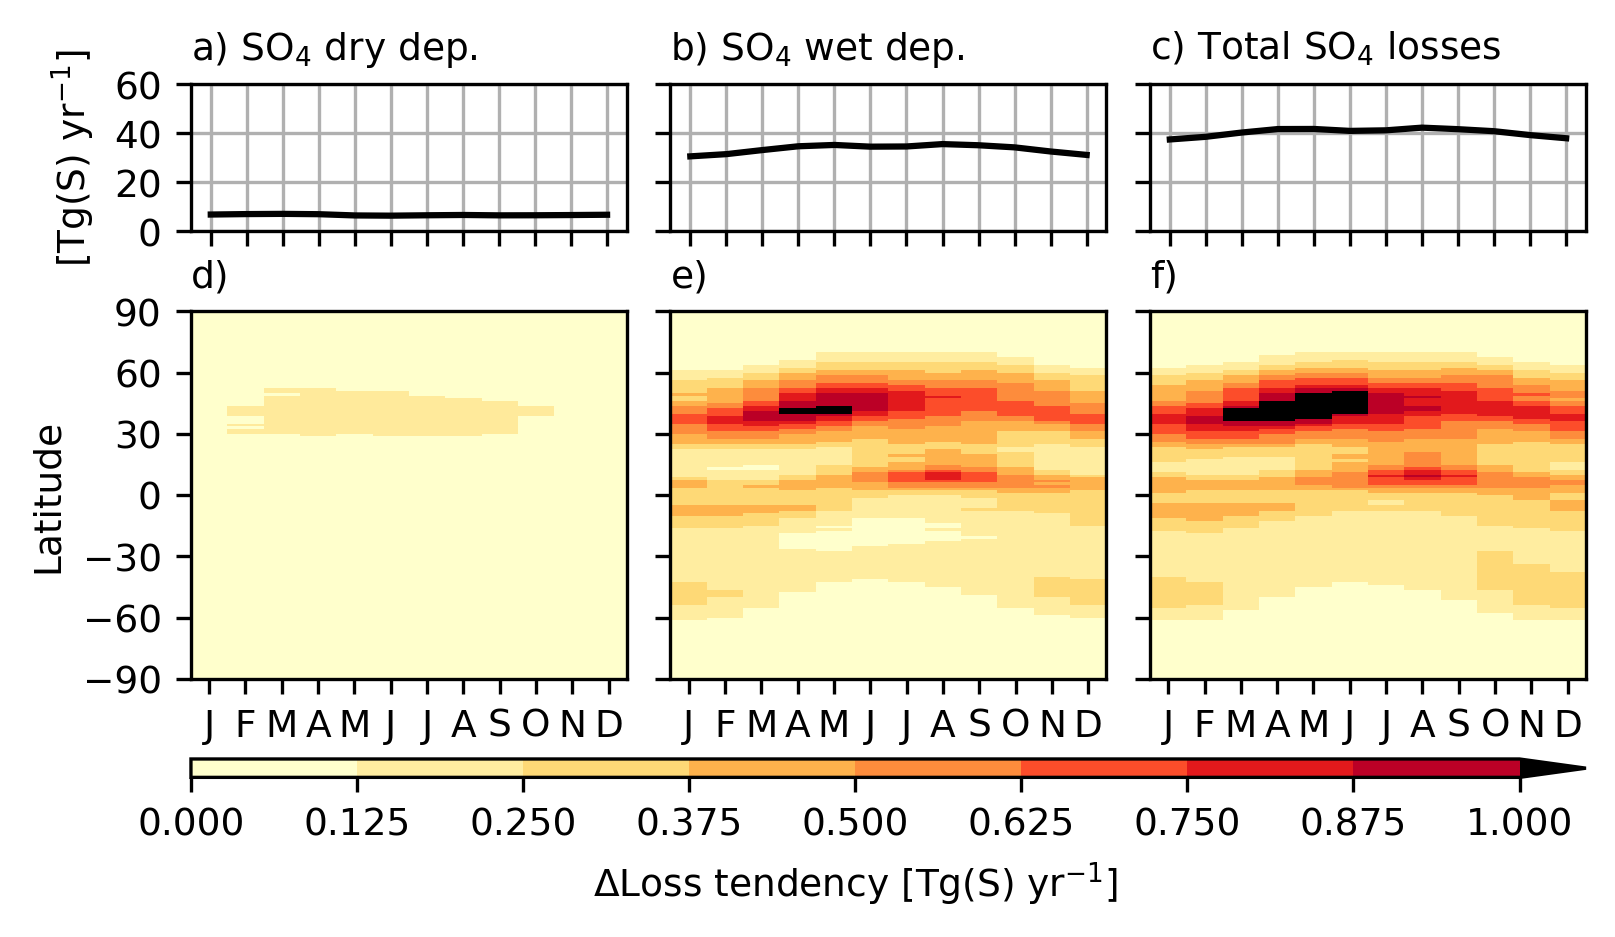
\includegraphics{Chapter4/Figs/so4_losses_histsst_pothole.png}
%     \caption[sulfate loss tendencies due to oxidation and deposition by months between 1960 and 1989 due to aerosol precursor emissions]{\ce{SO4} loss tendencies due to oxidation and deposition by months 1960 and 1989. (a-c) Total seasonal \ce{SO4} loss tendency. (d-f) \ce{SO4} loss tendency as a function of month of year and latitude. This plot is a difference between \histsst{} and \sstpiaer}
%     \label{fig:ch4:so4-loss}
% \end{figure}


\begin{figure}
    \centering
    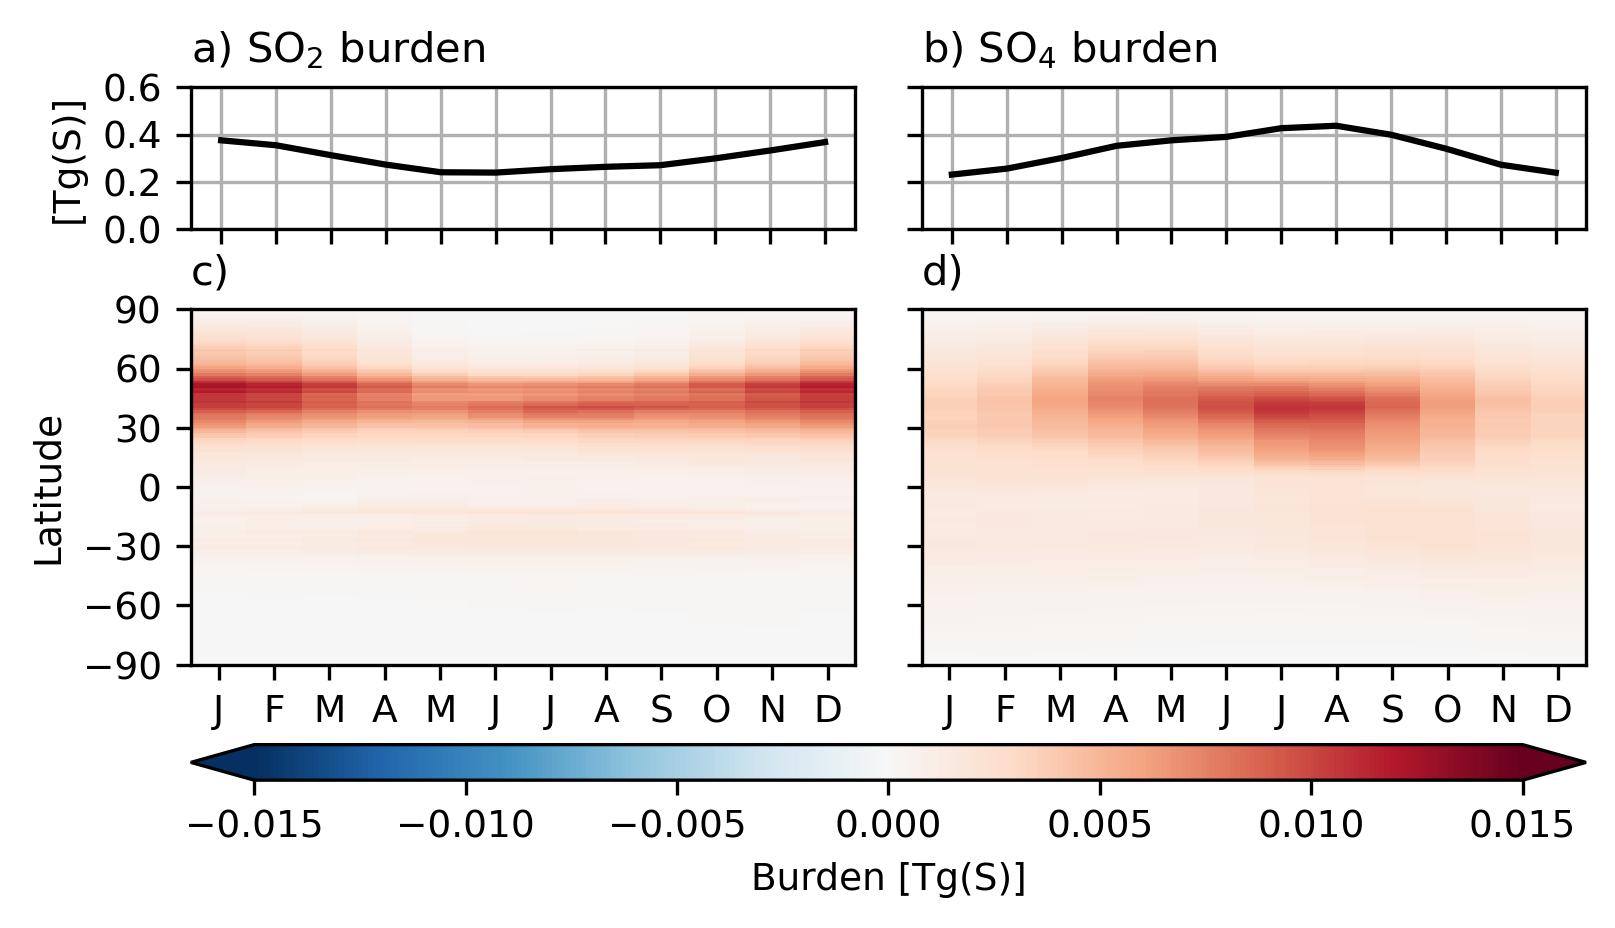
\includegraphics{Chapter4/Figs/seasonal_s_burden_pothole.png}
    \caption[\ce{SO2} and \ce{SO4} mass burden by season between 1960 and 1989]{\ce{SO2} and \ce{SO4} mass burden by season between 1960 and 1989 due to aerosol precursor emissions.}
    \label{fig:ch4:seasonal-s-burden}
\end{figure}

Changes in loss and production processes influence the sulfur burden. Figure \ref{fig:ch4:seasonal-s-burden} shows the change in \ce{SO2} and sulfate mass burden due to aerosol precursor emissions. In the northern hemisphere, where emissions are low, and oxidation is high in summer, there is a 0.15 Tg(S) decrease in \ce{SO2} burden and a subsequent increase in sulfate burden. The opposite is true when more \ce{SO2} is emitted in boreal winter, resulting in higher \ce{SO2} burden in December and January. The sulfate burden does not show a seasonal variation compared to the base sulfur burden without the increase in \ce{SO2} emissions during the pothole period.

\begin{figure}
    \centering
    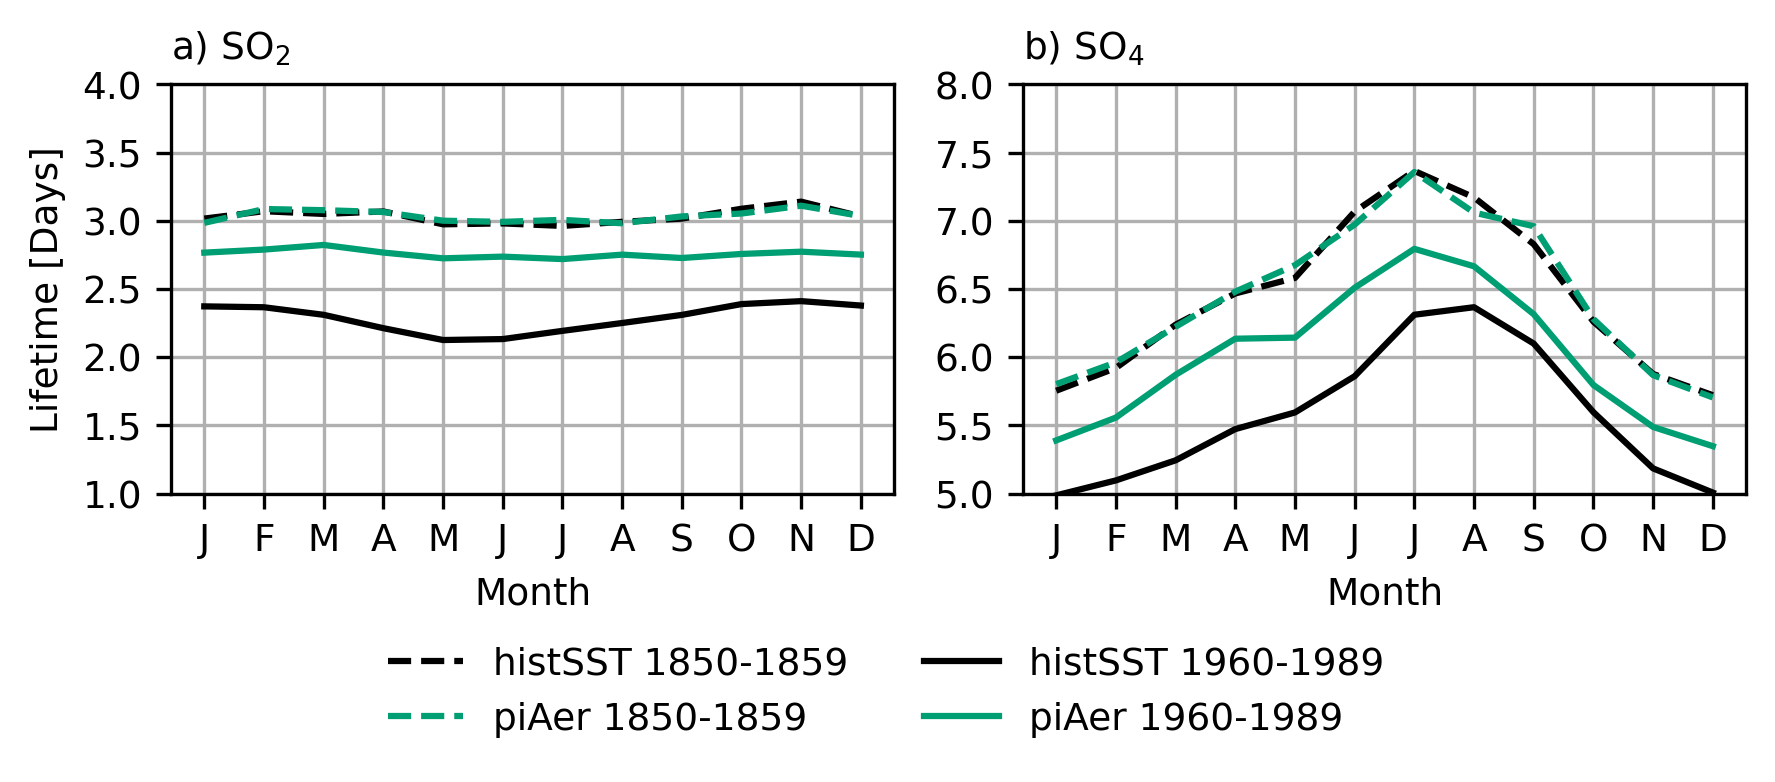
\includegraphics{Chapter4/Figs/lifetime_pothole.png}
    \caption[\ce{SO2} and \ce{SO4} lifetime by season between 1980 and 1989]{\ce{SO2} and \ce{SO4} lifetime by season between 1850--1859 and 1960--1989 from \histsst{} and \sstpiaer{}}
    \label{fig:ch4:seasonal-s-lifetime}
\end{figure}

Variation in loss mechanism modulates \ce{SO2} and sulfate burden and lifetimes. Figure \ref{fig:ch4:seasonal-s-lifetime} shows a global mean lifetime of \ce{SO2} and sulfate for two time periods, 1850--1859 and 1960--1989, aggregated by month. When \ce{SO2} emissions are at the 1850 level, \ce{SO2} lifetimes show a slight variation across seasons, as seen in both \sstpiaer{} trends (solid and dashed green lines) and \histsst{} (dashed black line) in the 1850s. Whether this slight variation is due to an additional 0.75 \unit{Tg(S)~yr^{-1}} of emission in winter (Figure \ref{fig:app1:seasonal-emiso2-1850}) or from the variation in loss processes is inconclusive. 

The higher oxidants in the atmosphere decrease the \ce{SO2} lifetime by increasing oxidation, as seen in Chapter \ref{ch3:title}. The average \ce{SO2} lifetime decreases from 3 days to 2.75 days when oxidant level increases in the 1980s even when \ce{SO2} emissions are constrained at the 1850s level as shown by the \sstpiaer{} simulation (dashed green line versus solid green line). \ce{SO2} emissions in the 1980s decreased its mean lifetime further by 0.75 days and exacerbated the seasonal variation compared to the 1850s. The lowest \ce{SO2} lifetime is observed in May and June of the pothole period, approaching 2.0 days from the original 3.0 days in the 1850s. It could be said that \ce{SO2} emission increase at the surface drives the lifetime down. 

Sulfate aerosol lifetime shows a greater variation across the season, even in the 1850s, with a shorter lifetime in winter at 5.7 days and a longer lifetime in summer at 7.3 days, showing a difference of 1.5 days between seasons. Majority of sulfate is formed from \ce{SO2} oxidation which is higher during summer months (at 30 \unit{Tg(S)~yr^{-1}} compared to 20 \unit{Tg(S)~yr^{-1}} in winter; Figure \ref{fig:ch4:so2-loss}). While sulfate wet deposition increases in summer, the rate of increase is lower than production (an increase of 5 \unit{Tg(S)~yr^{-1}} between winter and summer), resulting in a higher burden and longer lifetime. 

% Comment on the seasonal cycle of sulfate
Overall, this section shows that seasonal changes in oxidants, cloud fractions and depositions significantly affect the fate of \ce{SO2}. \ce{SO2} emitted in summer has a greater chance of being oxidised, especially by OH, forming new sulfate aerosol particles and affecting the climate. On the other hand, \ce{SO2} emitted in winter persists in the atmosphere as a more significant burden for a longer time and can potentially be air pollutants affecting the local population and the environment. 

\subsection{Seasonal changes of aerosol and cloud properties due to aerosol precursor emissions and their influence on radiative effects}

The greater proportion of \ce{SO2} being oxidised in the gas phase into sulfate aerosol affects the aerosol properties because \ce{SO2} oxidation and sulfate aerosol formation are coupled in UKESM1 through the GLOMAP-mode aerosol scheme. The scheme simulates aerosol mass and number independently, allowing the changes in oxidation to affect aerosol mass and number concentration. 

As described in the UKESM1 description paper, gas-phase oxidation of \ce{SO2} produces \ce{H2SO4}, which nucleates into new aerosols in nucleation mode \citep{mulcahyDescriptionEvaluationAerosol2020}. The aqueous-phase oxidation of \ce{SO2} is determined from the reaction of dissolved \ce{SO2} with \ce{H2O2} and \ce{O3} in cloud droplets. The model does not explicitly produce sulfate aerosols, but the reaction fluxes update the accumulation- and coarse-mode aerosol mass. In this way, aqueous-phase oxidation does not form new aerosol particles.

This section will attribute changes to aerosol and cloud properties to changes in \ce{SO2} oxidation. The multi-model study by \citet{thornhillEffectiveRadiativeForcing2021} showed that for the near-present period, the total aerosol ERF is \qty{-1.01}{W~m^{-2}}, with sulfate aerosol, BC, OC, contributing \num[]{-1.03}, \num[]{-0.25}, and \qty{0.15}{W~m^{-2}}, respectively. This shows \ce{SO2} contributes to 70\% of aerosol radiative effect. Since sulfate aerosol is the principal anthropogenic aerosol species regarding radiative effects, seasonal variation of aerosol properties and radiative balance would be attributable to \ce{SO2} oxidation. 

In addition, the seasonal cycles of carbonaceous aerosol precursor emissions are shown in the supplementary figures, Figure \ref{fig:app1:seasonal-emioa-pothole}, \ref{fig:app1:seasonal-emibvoc-pothole}, and \ref{fig:app1:seasonal-emibc-pothole}. The figures show that all other aerosol precursors either do not have significant seasonal variation or the emission locations do not overlap with \ce{SO2}. Organic aerosol emissions vary with seasons, but most OAs are emitted below 30\textdegree S. BC emissions vary between 6--8 \unit{Tg(C)~yr^{-1}} but the seasonal variation is negligible above 30\textdegree N.  Isoprene and monoterpene, which are the majority of BVOC emissions, are emitted from trees and are precursors to secondary organic aerosols. Most BVOCs are emitted between latitude 30\textdegree S and the equator, with minimal seasonal variation. Thus, it is safe to assume that, above 30\textdegree N, most aerosols are formed from \ce{SO2} emissions and that \ce{SO2} is the main driver for seasonal variation.


\subsubsection{Seasonal changes in aerosol properties due to aerosol precursor emissions}

This section examines the aerosol properties that result from oxidation in different seasons. To keep the relevant analysis together, a discussion on the historical changes and attribution to the increase in \ce{SO2} emissions are presented jointly.



\begin{figure}
    \centering
    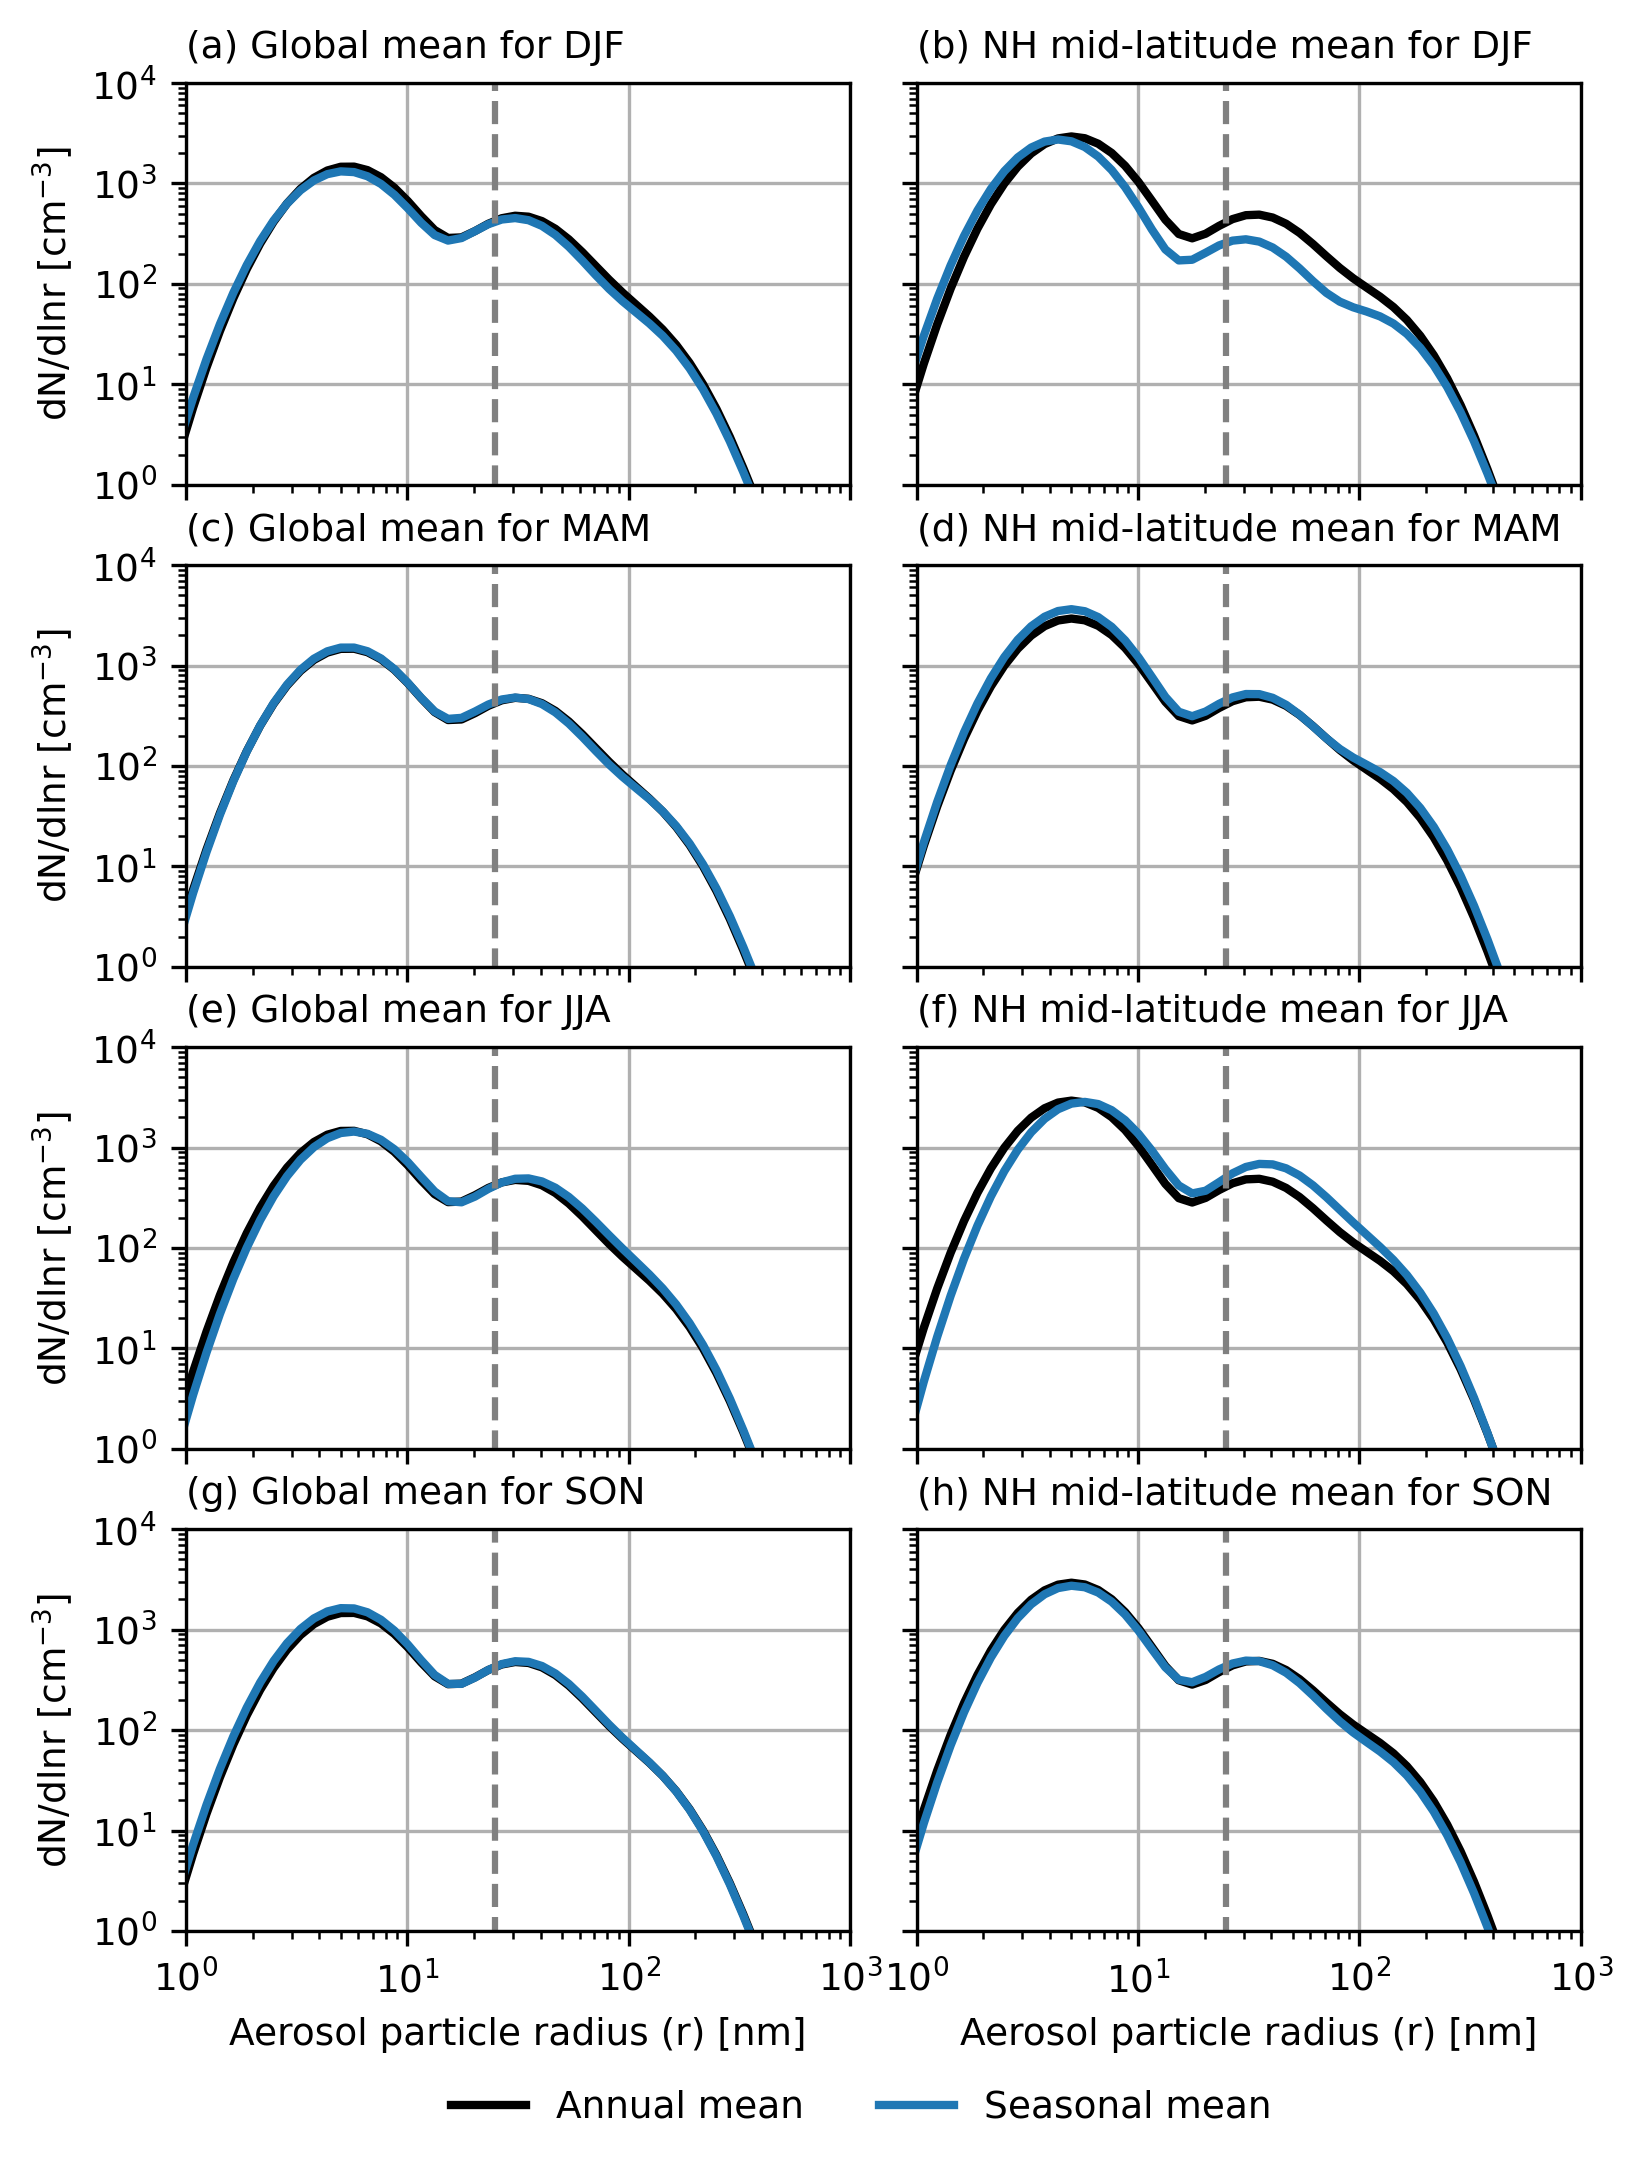
\includegraphics{Chapter4/Figs/seasonal_aerosol_size_dist_1980.png}
    \caption[Mean aerosol size distribution from the surface up to 10 km between 1980 and 1989 aggregated by seasons]{Mean aerosol size distribution from the surface up to 10 km between 1980 and 1989 aggregated by seasons. The black solid lines denote the domain annual mean. The blue lines denote the respective seasonal mean for each panel. The first column (sub-figure a, c, e, and g) shows the global mean aerosol size distribution. The second column (sub-figure b, d, f, and h) shows the mean between 30--60\textdegree N. The dashed vertical line indicates an aerosol radius of 25 nm, defined as N50 or aerosol with a diameter above 50 nm.}
    \label{fig:ch4:seasonal-aerosol-size}
\end{figure}


The seasonal variation in the oxidation pathway shows more gas-phase oxidation in boreal summer, which could affect aerosol formation. Figure \ref{fig:ch4:seasonal-aerosol-size} shows the variation in aerosol size distribution across the four seasons and a reference annual mean. The plots cover all aerosol components with aerosol size distribution up to accumulation mode aerosol ($\bar{r} = 1000$ \unit{\nano\metre} or $\bar{D} < 2000$ \unit{\nano\metre}) as coarse mode aerosol number concentration is negligible due to its low concentration. In the boreal summer months-- June, July and August (JJA)-- the global mean aerosol size distribution shows minor changes to global mean aerosol size distribution (left columns) in all seasons. However, the changes are more observable in the northern hemisphere mid-latitude (30\textdegree--60\textdegree N; right column). The aerosol size distribution in winter (December, January and February; DJF) is lower than the annual mean, especially for aerosol with a radius greater than 25 \unit{\nano\metre} or diameter above 50 \unit{\nano\metre} (N50), which acts as cloud condensation nuclei. The opposite is true for the same region over summer (June, July and August; JJA) when we have observed more gas-phase oxidation.


The \ce{SO2} oxidation pathways could explain the shift in aerosol size distribution in summer and winter and how the model simulates aerosol processes. In UKESM1, \ce{SO2} gas-phase reaction produces \ce{H2SO4} gas, which condenses into new nucleation mode aerosol particles \citep{mannDescriptionEvaluationGLOMAPmode2010}. On the other hand, \ce{SO2} aqueous-phase reactions add sulfate mass onto the existing aerosols in accumulation and coarse mode without forming new particles. The previous section shows that more \ce{SO2 + OH} reactions occur during summer. This additional aerosol particle production increases the accumulation mode (peaks at a 30 nm radius) aerosol number in summer. 


\begin{figure}
    \centering
    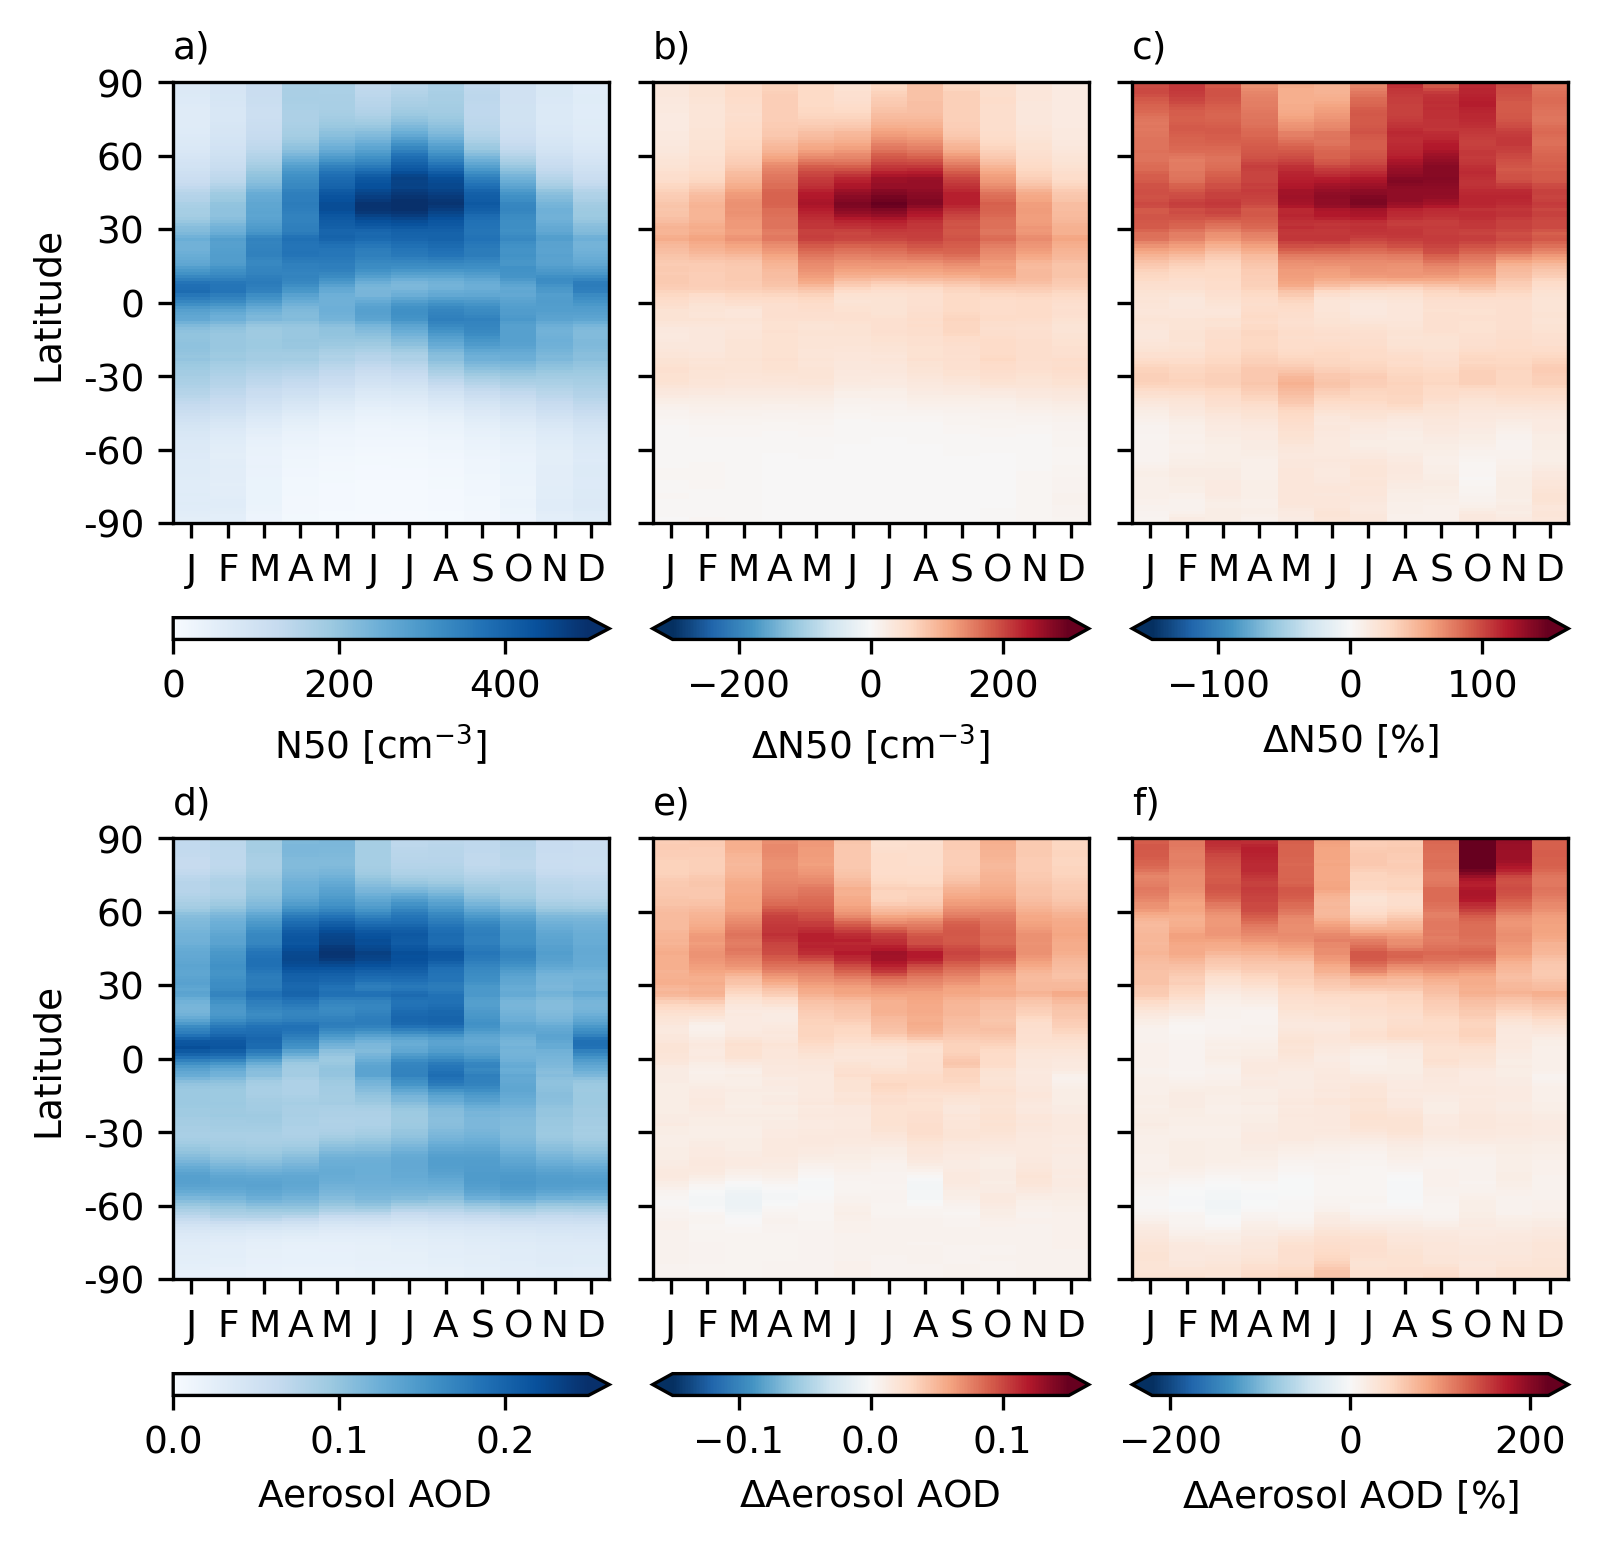
\includegraphics{Chapter4/Figs/seasonal_aerosol_props_1980.png}
    \caption[Mean AOD at 550 nm and N50 between 1980 and 1989 as a function of months and latitude due to aerosol precursor emissions]{mean (a--c) number concentration of aerosol with a diameter greater than 50 nm (N50) from the surface up to 10 km and (d--f) AOD at 550 nm between 1980 and 1980 as a function of months and latitude. The first column is the absolute value, and the second and third columns are the changes in aerosol properties due to aerosol precursor emissions (\histsst{} minus \sstpiaer{}) in absolute and relative terms, respectively.}
    \label{fig:ch4:seasonal-aerosol-props}
\end{figure}


Aerosol properties such as AOD and aerosol number concentration, especially those with a diameter above \qty{50}{nm} (N50), are linked to radiative forcing due to aerosols. AOD correlates with aerosol-radiation interaction and aerosol-cloud interaction, including aerosols of all sizes. N50 number concentration describes the available cloud condensation nuclei, which enhance the aerosol-cloud interaction. Figure \ref{fig:ch4:seasonal-aerosol-props} shows AOD and N50 number concentration and the changes due to aerosol precursor emissions below 10 km, roughly the tropopause's height. N50 number concentration is high in the tropics throughout the year at approximately 200 \unit{cm^{-3}} with a summer maximum between latitude 30 and 60\textdegree N. Figure \ref{fig:ch4:seasonal-aerosol-props}b and c show the change in N50 due to aerosol precursor emissions. The seasonal variation is attributed to aerosol precursor emissions, adding more than 200 \unit{cm^{-3}} or 150\% to N50 between June and August in the Northern Hemisphere. This seasonal variation is traced back to oxidation rather than emissions. There are more significant \ce{SO2} emissions in winter but a lesser growth in N50 of approximately 60\%.

Aerosol optical depth (AOD) quantifies the absorption or scattering of light by the aerosol layer in the atmosphere, providing a measure of aerosols' columnar concentration in the atmosphere. Figure \ref{fig:ch4:seasonal-aerosol-props}d, e, and f show AOD aggregated by latitude and months. AOD trend is similar to that of N50 number concentration characterised by a persistent band of high AOD in the equator and an elevated AOD in the summer between 30 and 60 \textdegree N. 

Studies show that UKESM1 and GLOMAP-mode, its aerosol component, are skilful in predicting sulfate aerosol variations between 1980 and 2009, with the tendency to underpredict sulfate aerosol concentration in Europe and East Asia compared to observations \citep{mannDescriptionEvaluationGLOMAPmode2010, mulcahyDescriptionEvaluationAerosol2020}. While UKESM1 predicts the spatial distribution of sulfate aerosol distribution, it consistently underpredicts the absolute values for all years, although it is within the observed variability. The model also underpredicts East Asian observations to a greater degree than GC3.1, a model with the same physical atmosphere-ocean and aerosol component but a lower level of interaction within the Earth system. 

UKESM1 features robust chemistry and aerosol interaction and reasonably agrees with a range of aerosol observations \citep{mulcahyDescriptionEvaluationAerosol2020}. However, UKESM1 overestimated surface \ce{SO2} concentration, which has been thought to be related to its dry deposition and caused the pothole cooling \citep{hardacreEvaluationSO2SO422021}. A new version of UKESM1, called UKESM1.1, has recently been released with a higher \ce{SO2} dry deposition to address this challenge \citep{mulcahyUKESM11DevelopmentEvaluation2023}. The new dry deposition scheme improved the surface air temperature prediction but has exacerbated the model's low bias in sulfate surface concentration \citep{hardacreEvaluationSO2SO422021}. As discussed in the next section, even with underpredicted sulfate aerosol, the model shows a substantial change in cloud properties compared to other Earth system models. 

\subsubsection{Seasonal changes in cloud properties due to aerosol precursor emissions}

Aerosol acts as cloud condensation nuclei, allowing water vapour to condense at lower temperatures than homogeneous nucleation. Thus, the change in aerosol number and size modifies cloud properties \citep[e.g. ][]{rosenfeldGlobalObservationsAerosolcloudprecipitationclimate2014, boucherCloudsAerosols2014,persadAerosolsMustBe2022}. Aerosol in the cloud increases its albedo and lifetime, leading to weather and climate effects \citep{twomeyInfluencePollutionShortwave1977, albrechtAerosolsCloudMicrophysics1989}.


% Why UKESM1 simulates cloud well
The aerosol scheme in UKESM1, GLOMAP-mode, uses a modal aerosol microphysics approach, accounting for aerosol mass and number while simulating key processes like nucleation and intermodal coagulation \citep{mannDescriptionEvaluationGLOMAPmode2010}. This enables a more detailed depiction of aerosol-cloud interactions and their radiative effects. GLOMAP-mode provides a better fit to observed aerosol optical depths, extends sulfate aerosol lifetime, and offers a more accurate prediction of aerosol-induced cloud changes \citep{bellouinImpactModalAerosol2013}. It demonstrates improved realism in simulating aerosol forcing and uncertainties associated with mass-based schemes. These improvements highlight the scheme's ability to refine climate models' assessments of aerosol impacts on climate systems.


\begin{figure}
    \centering
    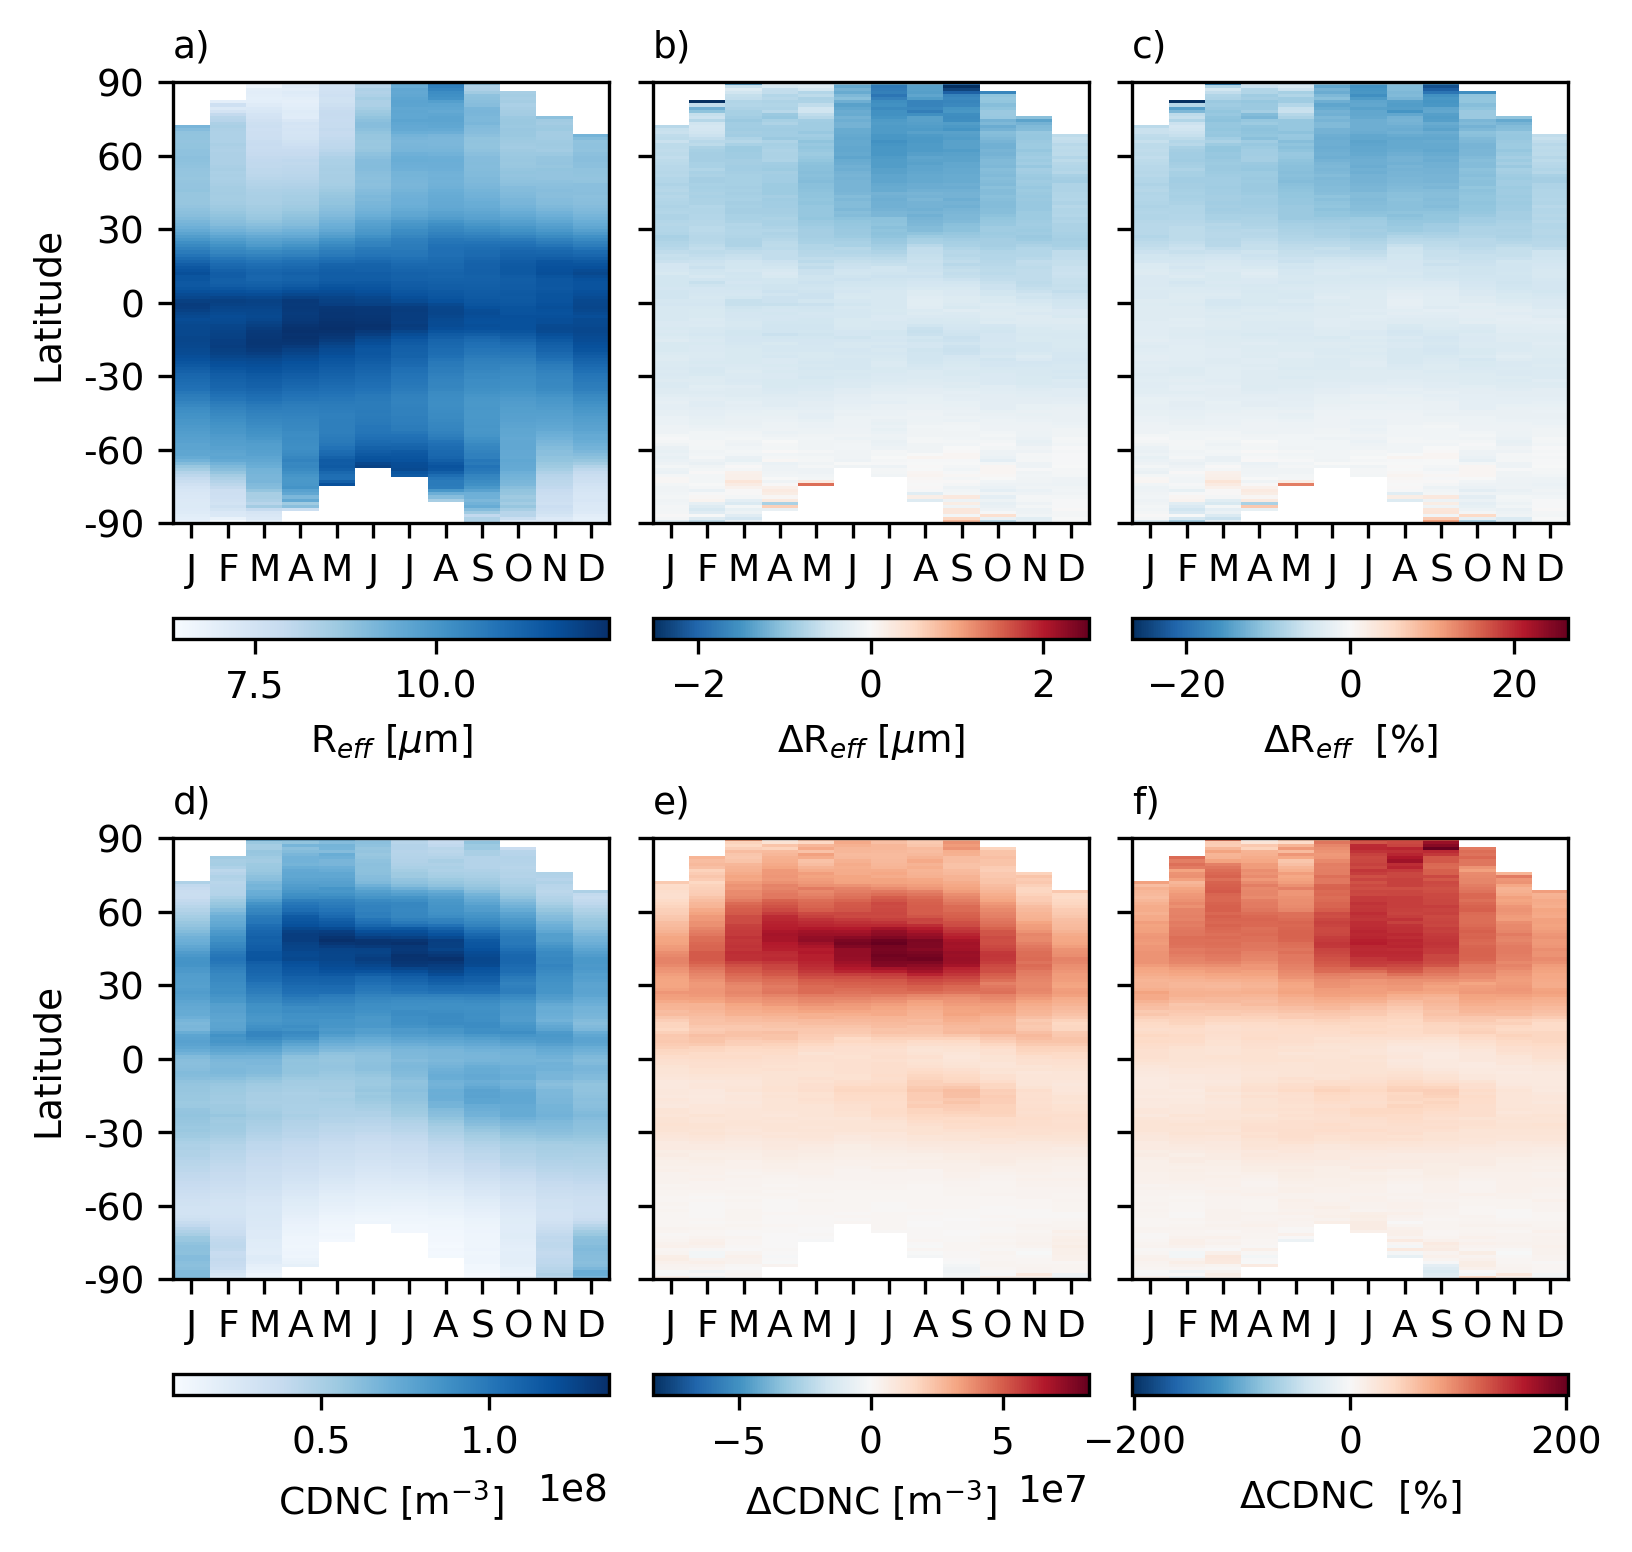
\includegraphics{Chapter4/Figs/seasonal_cloud_props1_pothole.png}
    \caption[\Reff{} and CDNC aggregated by latitude and month between 1960 and 1989]{a) shows mean \Reff{} from \histsst{} aggregated by latitude and month between 1960 and 1990 below 10 km. b-c) shows the change in \Reff{} due to aerosol precursor emissions (\histsst{} minus \sstpiaer{}) in absolute value and the percentage of change compared to \sstpiaer{}, respectively. d-f) show a similar analysis for CDNC.}
    \label{fig:ch4:seasonal-cloud-props1}
\end{figure}


Cloud droplet size and concentration are the two properties directly influenced by aerosols. Figure \ref{fig:ch4:seasonal-cloud-props1} shows the average cloud droplet effective radius and number concentration below 10 km aggregated by latitude and month. Cloud droplet effective radius, \Reff{}, forms a band at the equator due to equatorial convection. \Reff{}, at 30 to 60 \textdegree N decreases by approximately \qty{1.5}{\micro\metre} or 10\% between June and September due to aerosol precursor emissions. Cloud droplet number concentration has a strong increase in the boreal summer of the northern hemisphere mid-latitude. The increase is due to aerosol precursor emissions, increasing by 100\% at the same month and latitude. 


\begin{figure}
    \centering
    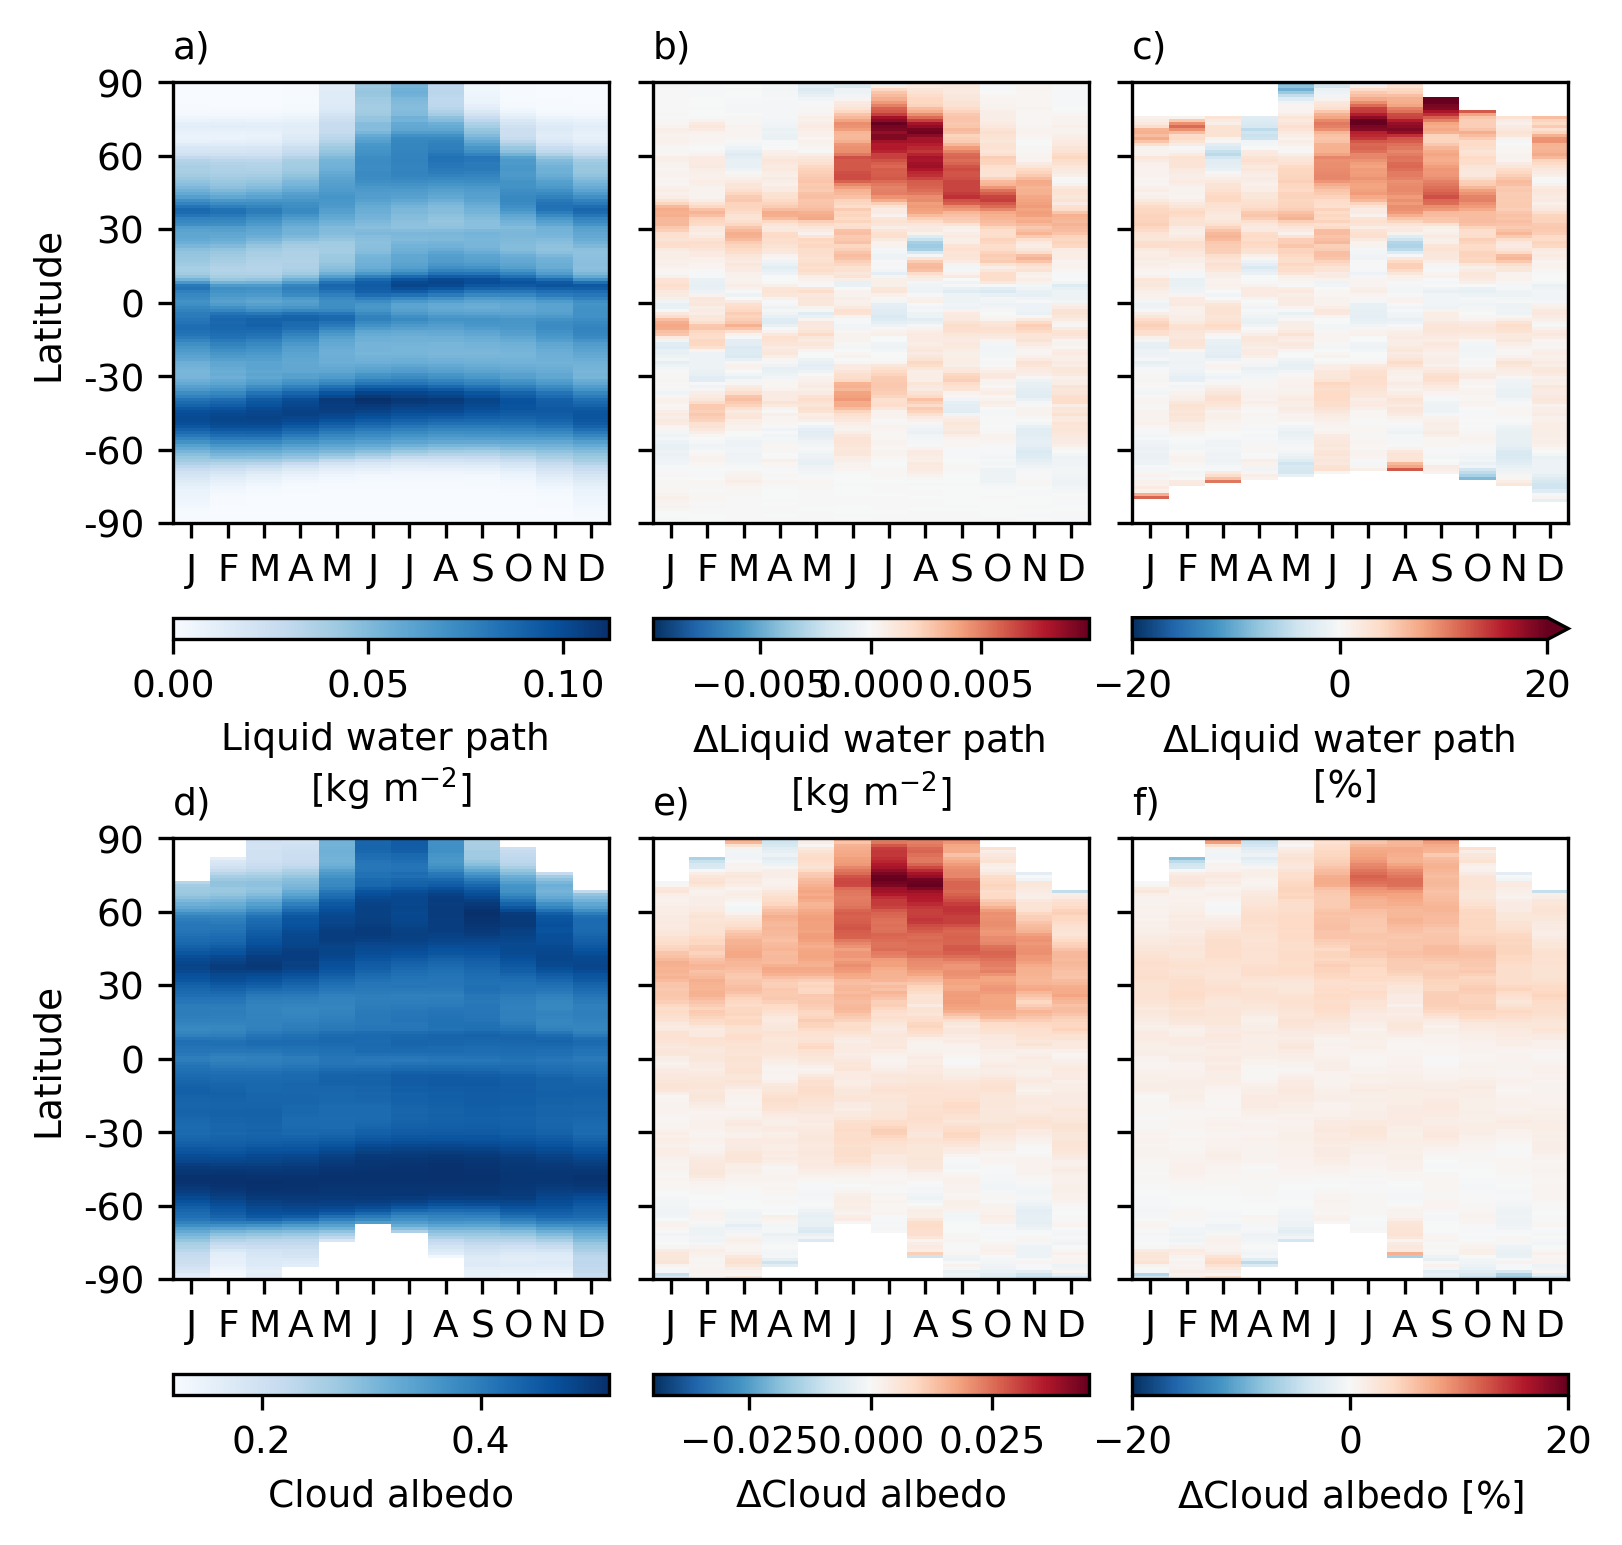
\includegraphics{Chapter4/Figs/seasonal_cloud_props2_pothole.png}
    \caption[Cloud liquid water path and albedo aggregated by latitude and month between 1960 and 1989]{a) shows mean liquid water path from \histsst{} aggregated by latitude and month between 1960 and 1990 below 10 km. b-c) shows the change in liquid water path due to aerosol precursor emissions (\histsst{} minus \sstpiaer{}) in absolute value and the percentage of change compared to \sstpiaer{}, respectively. d-f) show a similar analysis for cloud albedo.}
    \label{fig:ch4:seasonal-cloud-props2}
\end{figure}

Cloud reflectance increases as the droplet size decreases. Figure \ref{fig:ch4:seasonal-cloud-props2} shows the cloud liquid water path, the vertical integration of cloud liquid water content and cloud albedo grouped by latitude and months. Bands of clouds are persistent at the equator as well as at the 60 \textdegree S. However, between 1960 and 1989, the Northern Hemisphere mid-latitude band fluctuates in both latitude and thickness. The liquid water path in the northern hemisphere, especially during summer, increases by 15--20\% due to aerosol precursor emissions. 

Cloud albedo measures the reflectance of clouds at the top of the atmosphere. Figure \ref{fig:ch4:seasonal-cloud-props2}d shows that the mid-latitude clouds tend to be more reflective than the equatorial cloud. Aerosol precursor emissions enhance cloud albedo by 10\% in boreal summer. The result shows that the effect of aerosol precursors on cloud is localised and correlates to \ce{SO2} oxidation rather than emissions.


% Discuss cloud simulation in UKESM1 and any validations of this run
While the results above show substantial cloud response to aerosol precursors, most cloud properties simulated by UKESM1 exhibit a low bias compared to MODIS satellite measurements from March 2009 to March 2010 in the North Atlantic Ocean region \citep{grosvenorDecompositionCloudAerosol2020}. According to \citet{grosvenorDecompositionCloudAerosol2020}, the atmosphere-only version of UKESM1 can capture the cloud spatial pattern with a spatial correlation above 0.8 but consistently underestimates cloud cover and liquid water path. Low- and mid-altitude cloud fraction is lower by a normalised mean bias factor (NMBF) of -28--37\%. The high altitude cloud is the least biased at -8.5\%. In-cloud liquid water path is also underestimated with NMBF of -20\%. In contrast, cloud droplet number concentration is overestimated by 11.3\%.


It is essential to note that UKESM1 has the largest change in cloud fraction from aerosol precursor emissions amongst 6 ESMs with interactive chemistry and aerosol schemes that participated in AerChemMIP \citep{zhangRoleAnthropogenicAerosols2021}. While UKESM1 underestimates cloud fraction, it is also the most sensitive to changes in aerosol loading \citep{zhangRoleAnthropogenicAerosols2021}, but model aerosol sensitivity does not predict pothole cooling. More comparison is needed between models to diagnose the underpinning aerosol and process that leads to pothole cooling. 


\subsection{Seasonal variation of ERF due to aerosol precursor emissions and the specific ERF in different seasons}

So far, this chapter has shown that \ce{SO2} emissions increase with more energy demands during boreal winter, but aerosol formation does not follow seasonal emission variations. Instead, new sulfate aerosol particles form when more OH is present to drive gas-phase reactions, leading to more aerosol number concentration and brighter clouds in boreal summer. This section discusses the seasonal variation in aerosol-radiation interaction and establishes the correlation between ERF and oxidation processes. Finally, it shows quantitatively that the emission timing is responsible for more negative ERF in summer using the concept of specific ERF.


\begin{figure}
    \centering
    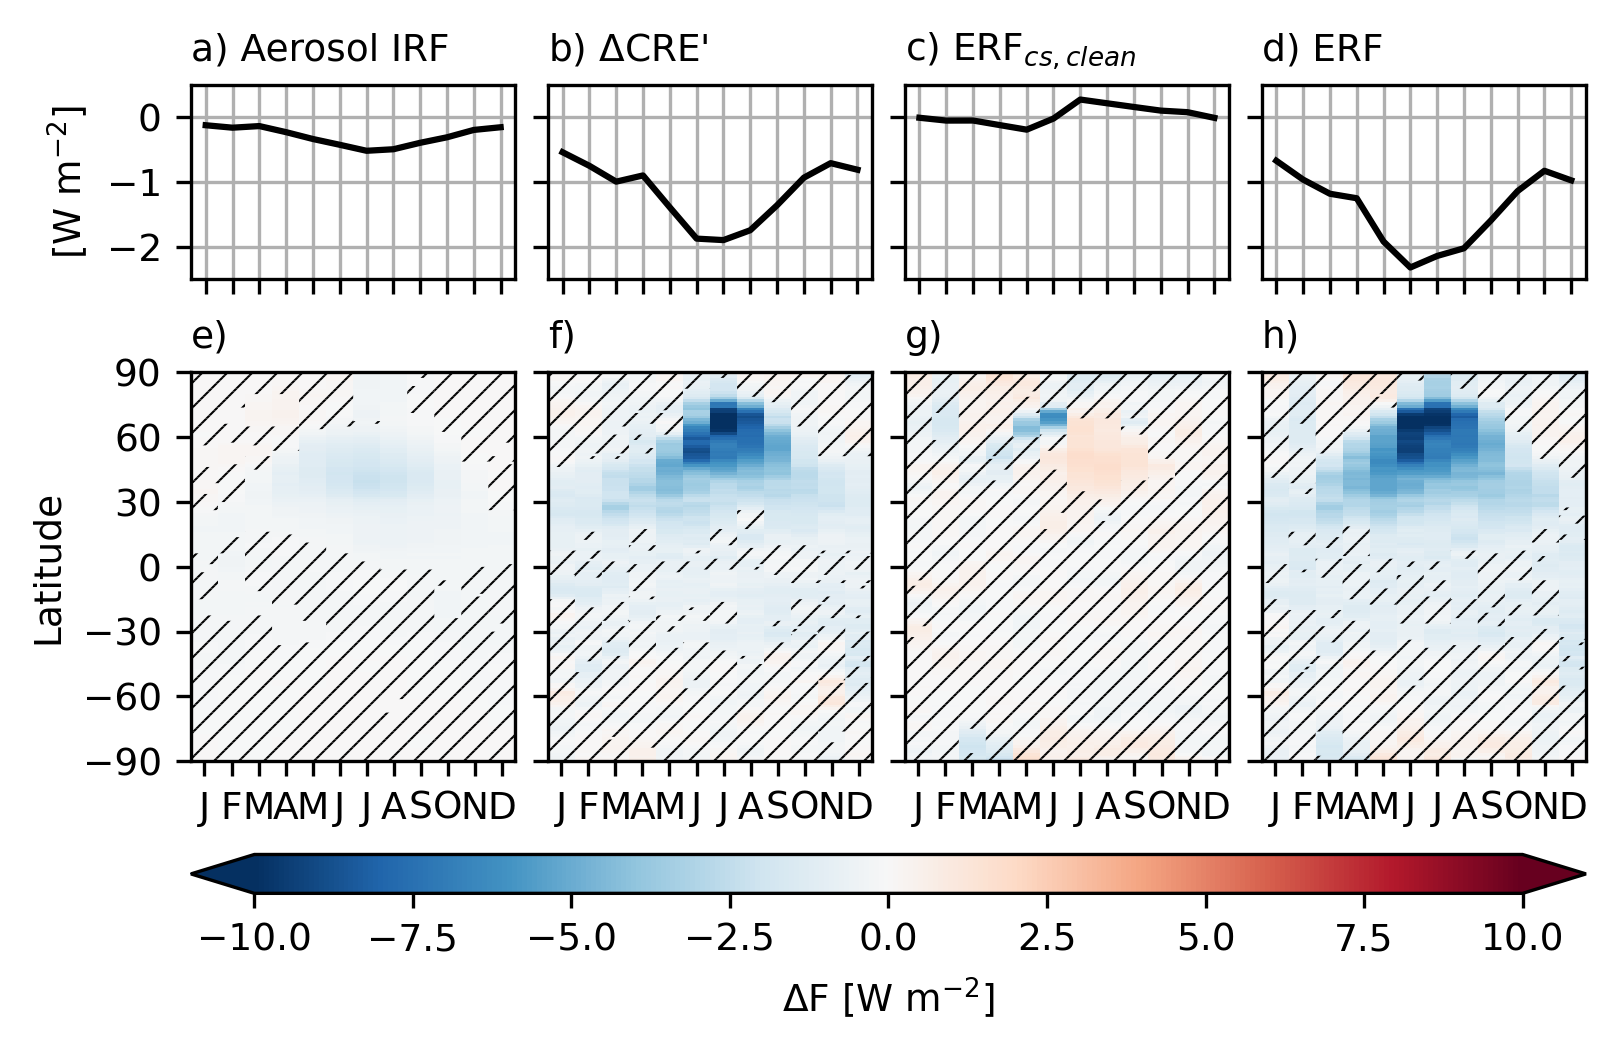
\includegraphics{Chapter4/Figs/latitudinal_erf_sstpiaer-histsst_pothole.png}
    \caption[ERF due to aerosol precursor emissions between 1960--1989 aggregated by month and latitude]{ERF due to aerosol precursor emissions between 1960--1989 aggregated by month and latitude. Each data point is averaged longitudinally, giving 10 data points for each month and latitude. Hatch denotes points where the difference between \histsst{} and \sstpiaer{} is insignificant (p$\leq$0.05).}
    \label{fig:ch4:seasonal-erf}
\end{figure}

Aerosol-radiation and aerosol-cloud interactions are the main drivers for radiative imbalance at the top of the atmosphere due to aerosol precursor emissions. These effects are quantified using ERF. Figure \ref{fig:ch4:seasonal-erf} shows ERF and its components due to aerosol precursor emissions aggregated by month and latitude. ERF shows a strong seasonal variation with a high negative in the boreal summer between 1960 and 1989 when \ce{SO2} oxidation is the greatest annually. Aerosol radiative impact is less significant in boreal winter even though \ce{SO2} emission is the strongest in winter, contrary to the assumed correlation between emissions and ERF. 

ERF could be decomposed into its aerosol scattering component or the aerosol (aerosol instantaneous radiative forcing; IRF), the cloud radiative effects (CRE') and the clean-and-clear sky part (ERF\textsubscript{cs,clean}), as described in section \ref{sec:ch2:erf}. ERF\textsc{cs,af} is the total clear-sky non-cloud adjustment without greenhouse gas changes. The decomposition of ERF shows that aerosol significantly enhances the cloud radiative effects in summer, accounting for \qty{-2}{W~m^{-2}} or 80\% of total ERF. IRF is responsible for \qty{-0.5}{W~m^{-2}} in the same season. The cooling effect is partially offset by the ERF\textsubscript{cs,clean} which is \qty{0.25}{W~m^{-2}}. \citet{ghanTechnicalNoteEstimating2013} attributes this mostly to the surface albedo change. The positive adjustments due to aerosol are from the tropospheric temperature and surface temperature adjustments, which contribute 0.023 and \qty{0.049}{W~m^{-2}}, respectively, in the case of the near-present aerosol forcing \citep{thornhillEffectiveRadiativeForcing2021}. 


% Discuss the ERF from different cloud adjustments
Aerosol radiative effects act mainly in the shortwave \citep{thornhillEffectiveRadiativeForcing2021,grosvenorDecompositionCloudAerosol2020}. The atmosphere-only version of UKESM1 shows a negative bias in low-altitude cloud fraction with -28.1\% NMBF while overestimating shortwave outgoing radiation at the top of the atmosphere by 1.7--5.8\% NMBF compared to the MODIS satellite observation in the present-day simulation \citep{grosvenorDecompositionCloudAerosol2020}. CDNC is underestimated in the northern North Atlantic Ocean region but overestimated in the southern North Atlantic Ocean by 21.5\%. However, this does not contribute substantially to the bias of outgoing shortwave radiation at the top of the atmosphere \citep{grosvenorDecompositionCloudAerosol2020}. This shows that the model predicts a radiation response from clouds over the Northern Atlantic that is too strong. Whether this correlation applies to other regions is unknown.


\begin{figure}
    \centering
    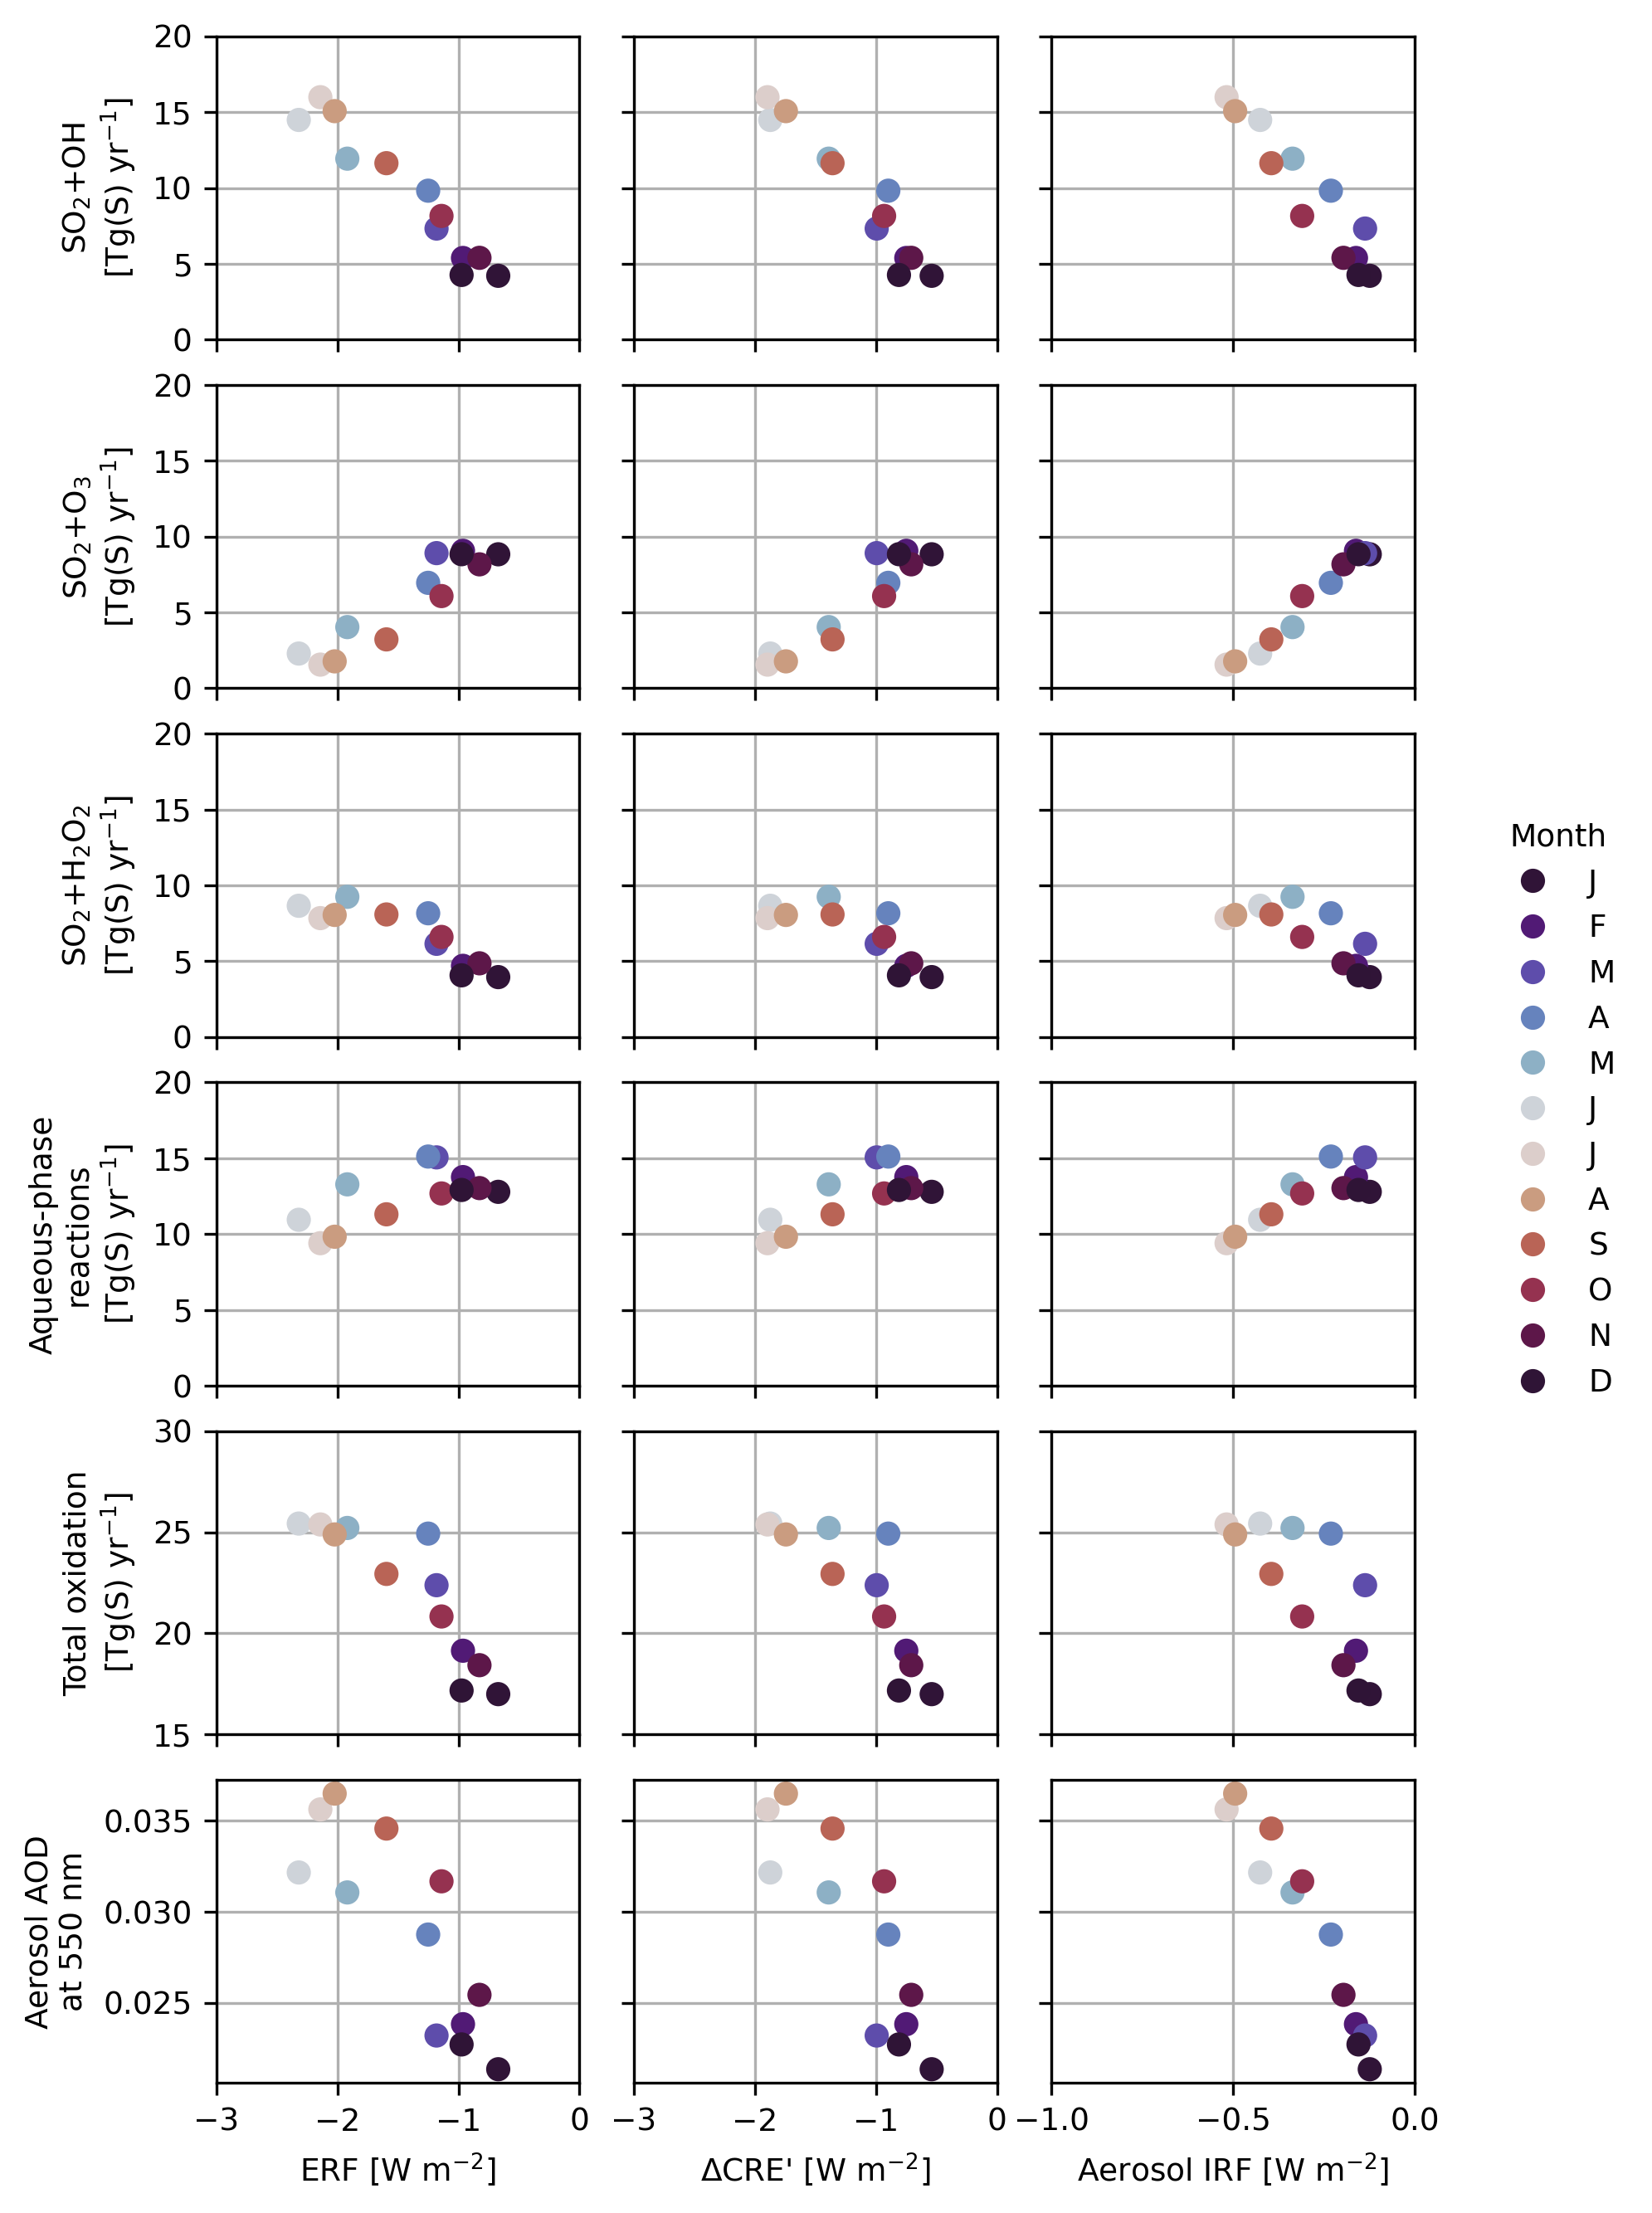
\includegraphics[width=\linewidth]{Chapter4/Figs/seasonal_oxidation_erf_corr_pothole.png}
    \caption[Correlation between \ce{SO2} oxidation tendencies and ERF between 1960 and 1989]{Scatter plots comparing global mean data aggregated by month between 1960 and 1989 for (vertical) \ce{SO2} oxidation tendencies, AOD and (horizontal) ERF }
    \label{fig:ch4:seasonal-erf-corr}
\end{figure}

As many parameters, such as oxidation and aerosol properties, show seasonal variations, it may be insightful to understand the correlation between the parameters and the resulting radiative forcing. Figure \ref{fig:ch4:seasonal-erf-corr} shows the correlation between oxidation, AOD and radiative forcing to address if there is a linear correlation between terms. Each plot shows the global mean oxidation and AOD aggregated by month and the global mean ERF for the same month. \ce{SO2 + OH} is inversely correlated with ERF and its components, showing greater oxidation tendency and more negative ERF in June--August. Neither total oxidation nor aerosol AOD correlate well with ERF. This suggests that gas-phase oxidation is a valuable parameter for this type of analysis. This plot indicates that oxidation tendencies explain ERF and not emission.


Although simulations targetting \ce{SO2} emissions during the pothole do not exist, using apportionment simulations for the near-present emissions, it is reasonable to assume that \ce{SO2} is the main contributor to aerosol precursor emission ERF. Near-present aerosol ERF apportionment indicated that 70.1\% of aerosol precursor ERF is due to \ce{SO2} emissions \citep{thornhillEffectiveRadiativeForcing2021}. For the near-present aerosol precursor emissions, ERF due to all aerosol precursors was \qty{-1.10}{W~m^{-2}}, of which \qty{-1.36}{W~m^{-2}} was from \ce{SO2} emissions, \qty{-0.21}{W~m^{-2}} is from organic carbon aerosols, and \qty{0.37}{W~m^{-2}} was from black carbon aerosols. \ce{SO2} emissions peaked in the 1980s compared to total aerosol precursor emissions  \citep{hoeslyHistorical175020142018} and the ratio of \ce{SO2} emission to total emissions has decreased for the near-present period. So, it is safe to assume that \ce{SO2} contributed more than 70\% of total ERF during the pothole period.

\begin{figure}
    \centering
    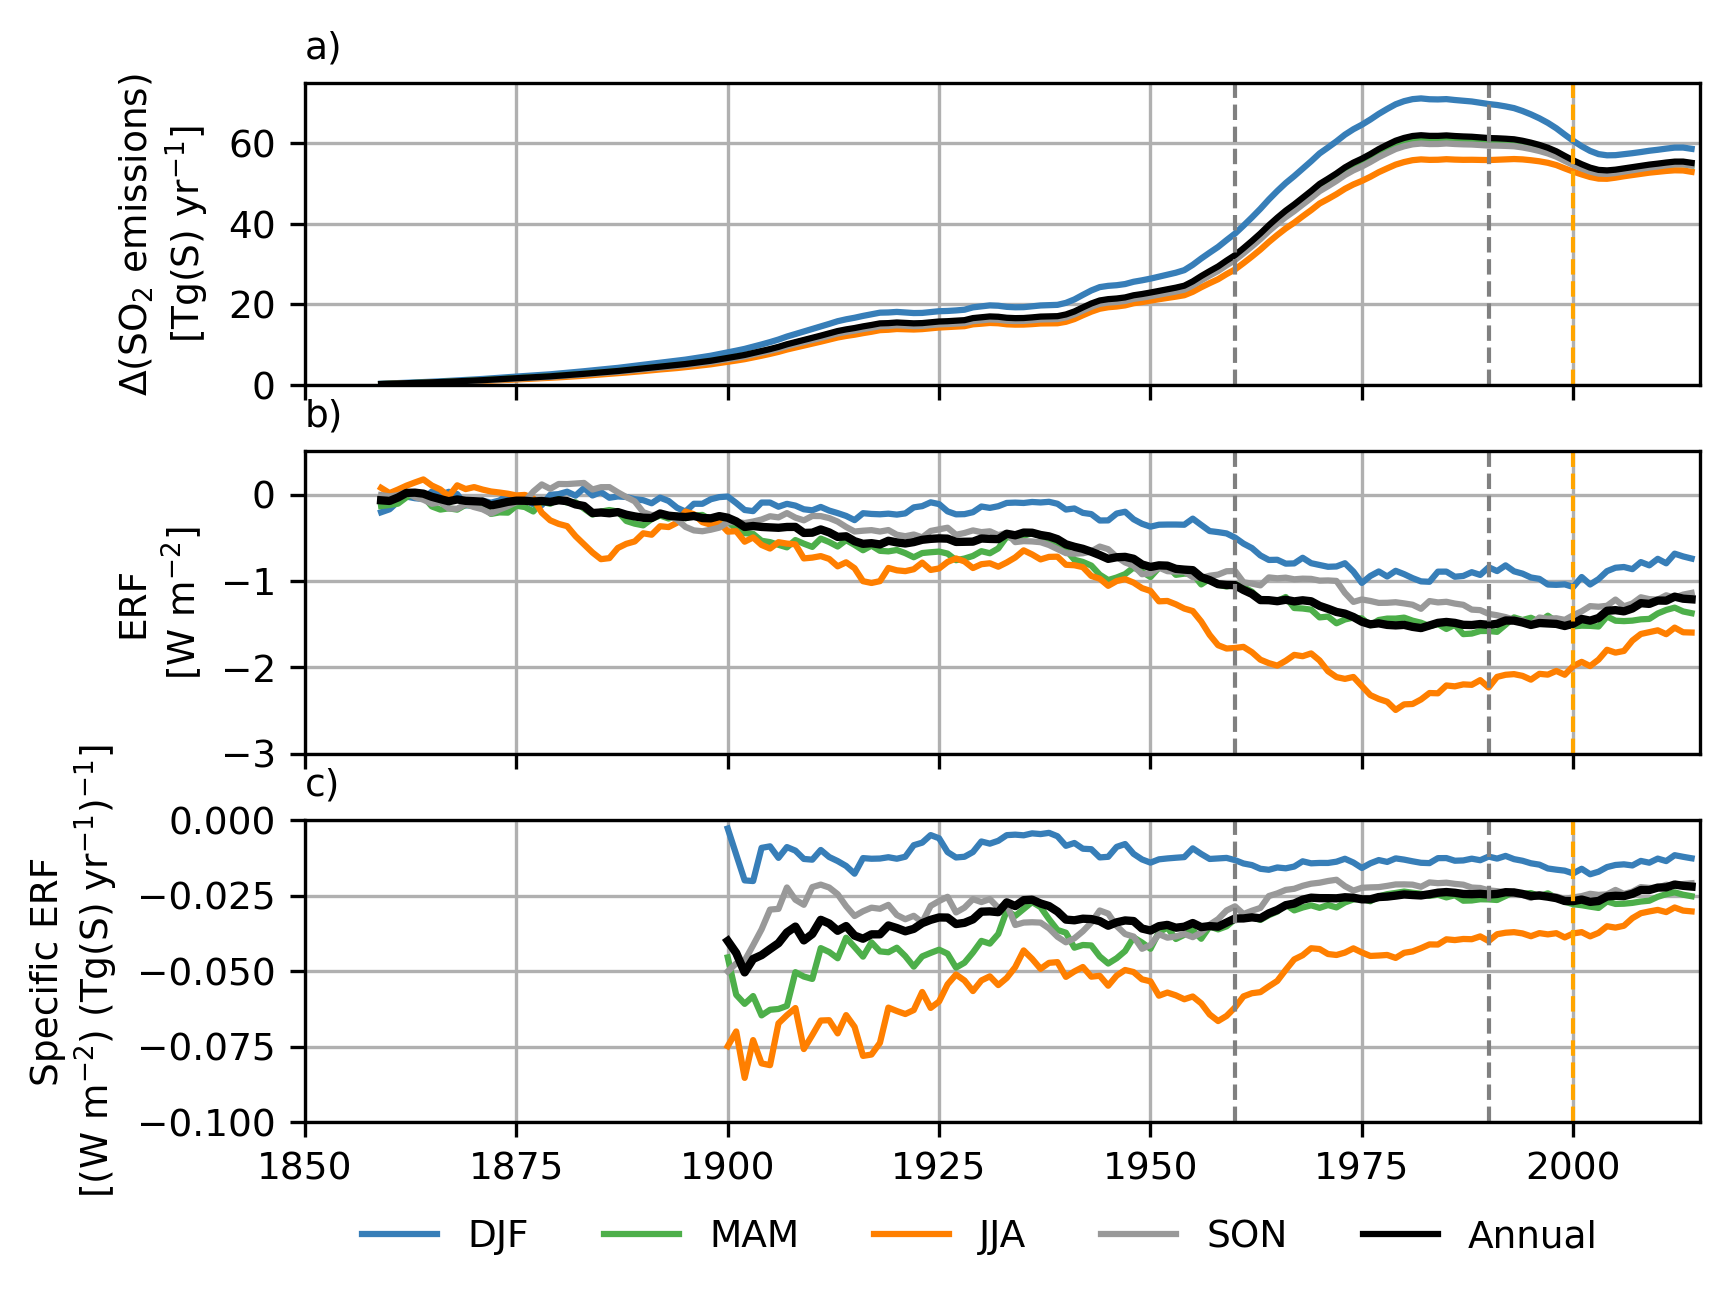
\includegraphics{Chapter4/Figs/seasonal_specific_erf.png}
    \caption[Specific ERF aggregated by seasons between 1900--2014]{Evolution of a) \ce{SO2} emissions due to aerosol precursor emissions (i.e. \histsst{} minus \sstpiaer{}). b) ERF and c) specific ERF (ERF per emitted \ce{SO2} aggregated by seasons) due to aerosol precursor emissions. All data have been applied with a 10-year rolling average. Specific ERF is shown for 1900 onwards due to high noise from a small denominator. Dashed grey lines are the start and end of the pothole period (1960--1989 inclusive), while the dashed orange line denotes the start of the near-present period (2000).}
    \label{fig:ch4:specific-erf}
\end{figure}

Due to the nature of the available oxidants and cloud fraction, \ce{SO2} emitted in summer is more likely to be oxidised and form sulfate aerosol. Specific ERF, the ERF per unit of \ce{SO2} emissions, could quantify this effect, as shown by \citet{bellouinRegionalSeasonalRadiative2016}. Figure \ref{fig:ch4:specific-erf} describes the evolution of global mean \ce{SO2} emissions, ERF, and specific ERF per unit of \ce{SO2} emissions in four seasons. Assuming that \ce{SO2} emission is the primary driver of aerosol precursor ERF, during the pothole period, each teragram of sulfur emission releases in summer contributes to 4 times more cooling than the same amount emitted in winter (\num{-0.05} compared to \qty{-0.0125}{(W~m^{-2})~(Tg(S)~yr^{-1})^{-1}}). Specific ERF in autumn (SON), winter (DJF) and spring (MAM) show less temporal variation compared to summer, averaging at \qty{-0.0125}{(W~m^{-2})~(Tg(S)~yr^{-1})} in winter and \qty{-0.025}{(W~m^{-2})~(Tg(S)~yr^{-1})} in spring and autumn of the pothole period. Summertime specific ERF (JJA) decreases over time from  \qty{-0.05}{(W~m^{-2})~(Tg(S)~yr^{-1})} during the pothole period to \qty{-0.035}{(W~m^{-2})~(Tg(S)~yr^{-1})}; yet it remains at least double that of winter.


% Note on Bellouin's 2016 work on specific RF. 
According to a multi-model study of specific aerosol ERF, HadGEM3, a lower complexity model which also uses GLOMAP-mode as its aerosol scheme, simulated the strongest specific ERF due to \ce{SO2} of the four models included \citep{bellouinRegionalSeasonalRadiative2016}. HadGEM3 showed the most negative specific ERF in summer when emissions were from Europe, at \qty{-0.036}{(W~m^{-2})~(Tg(S)~yr^{-1})^{-1}} \citep{bellouinRegionalSeasonalRadiative2016}. This is less negative than summer specific ERF from UKESM1 during the pothole period obtained in this chapter of \qty{-0.05}{(W~m^{-2})~(Tg(S)~yr^{-1})^{-1})}. HadGEM3 and UKESM1 are similar, employing the same physical component and aerosol scheme, amongst other components. This similarity implies that the UKESM1 may also have a high sensitivity to \ce{SO2} emission on aerosol-radiation interaction compared to other models.


\subsection{Surface air temperature anomaly and connection to aerosol effective radiative forcing}
\label{ch4:sec:seasonal-tas}

Aerosol-radiation interaction enhances the scattering of outgoing shortwave radiation, resulting in a negative ERF, which is shown to be stronger in summer. Aerosol asserts its radiative effects close to its emission source due to its short lifetime, resulting in cooler surface temperature. There is ample evidence of aerosol impact on surface temperature in diurnal time scale across seasons \citep[e.g. ][]{hanMechanismsSeasonalDifferences2020}. For example, aerosols reduce the global terrestrial mean diurnal temperature range by 0.47 K, with almost half the contribution coming from aerosols of anthropogenic origin \citep{chakrabortyLandCoverRegulates2019}. However, contrasting evidence exists on the effects of aerosol on surface temperature on a global and longer temporal span. 

Aerosol's effect on atmospheric temperature is local. For example, anthropogenic aerosols indirectly increase surface temperature and decrease the diurnal temperature range in East Asia by reducing shortwave solar radiation and rising cloudiness and cloud liquid water \citep{huangImpactAerosolIndirect2006}. Aerosol causes changes in local air temperature, as observed in the urban heat island effect on a short time scale and regional scale \citep{hanMechanismsSeasonalDifferences2020}. Aerosols reduce urban heat island intensity in summer by cooling down surface temperature more strongly in urban areas than in rural areas but increase it in winter by weakening heat transport and expanding the planetary-boundary-layer stability. 

While aerosol affects radiation budget locally and temporally on a short time scale, change in surface temperature does not have a simple localised or linear response to aerosol perturbation. Modelling studies show that sea surface temperature change due to aerosol shows a similar pattern to homogeneous forcing, i.e. greenhouse gases \citep{xieSimilarSpatialPatterns2013,kasoarSimilarSpatialPatterns2018}. Aerosols from different industrial regions (North America, Europe, East and South Asia) cause significant cooling across the hemisphere, showing a consistent spatial pattern of temperature changes regardless of the emission source \citep{kasoarSimilarSpatialPatterns2018, lewinschalLocalRemoteTemperature2019}.  

Acknowledging the multifaceted challenges, this section explores simulated surface air temperature and compares it to observations to diagnose its possible connection to pothole cooling observed between 1960 and 1980. To understand the impact of aerosol precursor emissions, the following analysis benefits from the historical coupled atmosphere-ocean simulations as they allow for changes in the surface temperature due to aerosol forcing. \hist{} is the historical simulation with all historical emissions, while \histpiaer{} has all its aerosol precursor emissions set to 1850. The difference between the two simulations allows for investigating the aerosol precursor's impact on the Earth system.

\begin{figure}
    \centering
    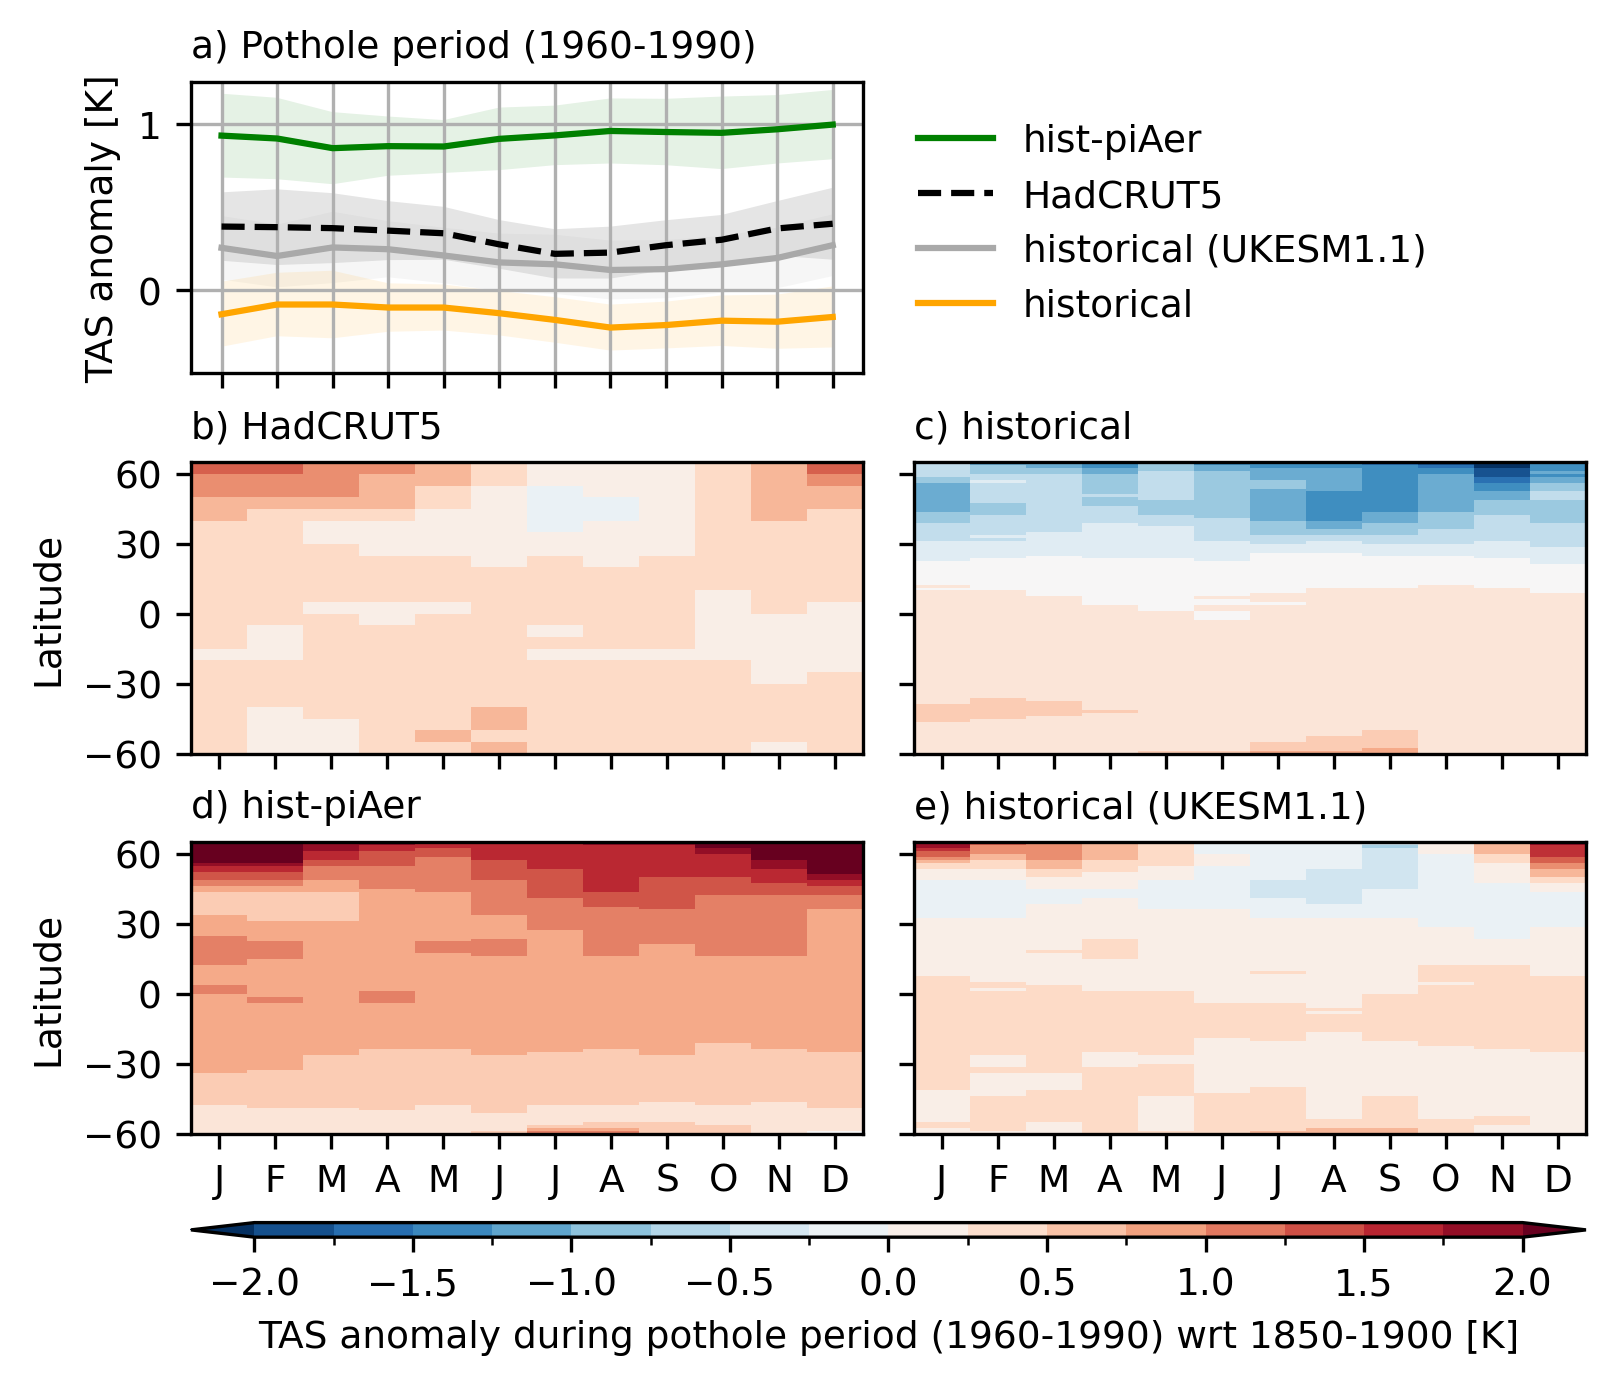
\includegraphics{Chapter4/Figs/TAS_anomaly_pothole.png}
    \caption[Surface air anomaly from HadCRUT5, UKESM1 and UKESM1.1 between 1960 and 1989]{a) mean surface air temperature anomaly between 1960--1989 with respect to 1850--1899 averaged over latitude 60\textdegree S and 65\textdegree N aggregated by month. b) surface air temperature anomaly from HadCRUT5 adjusted to 1850--1899. c-e) shows surface air temperature from UKESM1 c) \hist{} and d) \histpiaer{} simulation. d) is the same as c but from UKESM1.1. }
    \label{fig:ch4:seasonal-tas-anomaly-pothole}
\end{figure}

First, the seasonal cycle of surface air temperature (TAS) anomaly is examined. TAS anomaly is the deviation from its 1850--1899 climatology. The original HadCRUT5 dataset provides temperature anomalies with respect to the period 1900--1949. In Figure \ref{fig:ch4:seasonal-tas-anomaly-pothole}, the HadCRUT5 anomaly is readjusted to 1850--1899 to be comparable with the UKESM1 simulation and to show the depth and extent of the pothole cooling in the model compared to observation. The figure shows the seasonal variation of TAS from HadCRUT5 and model simulations. The surface temperature is aggregated by latitude between 60 \textdegree S and 65 \textdegree N and month. HadCRUT5 shows a seasonal variation in TAS with the lowest temperature observed between June and September between Latitude 30 and 60 \textdegree N. UKESM1 captures this variation but underestimates TAS globally. In contrast, the TAS anomaly in \histpiaer{} shows a different seasonal variation with the lowest anomaly in March. This indicates that aerosols influence the seasonal variation in TAS. 


\begin{figure}
    \centering
    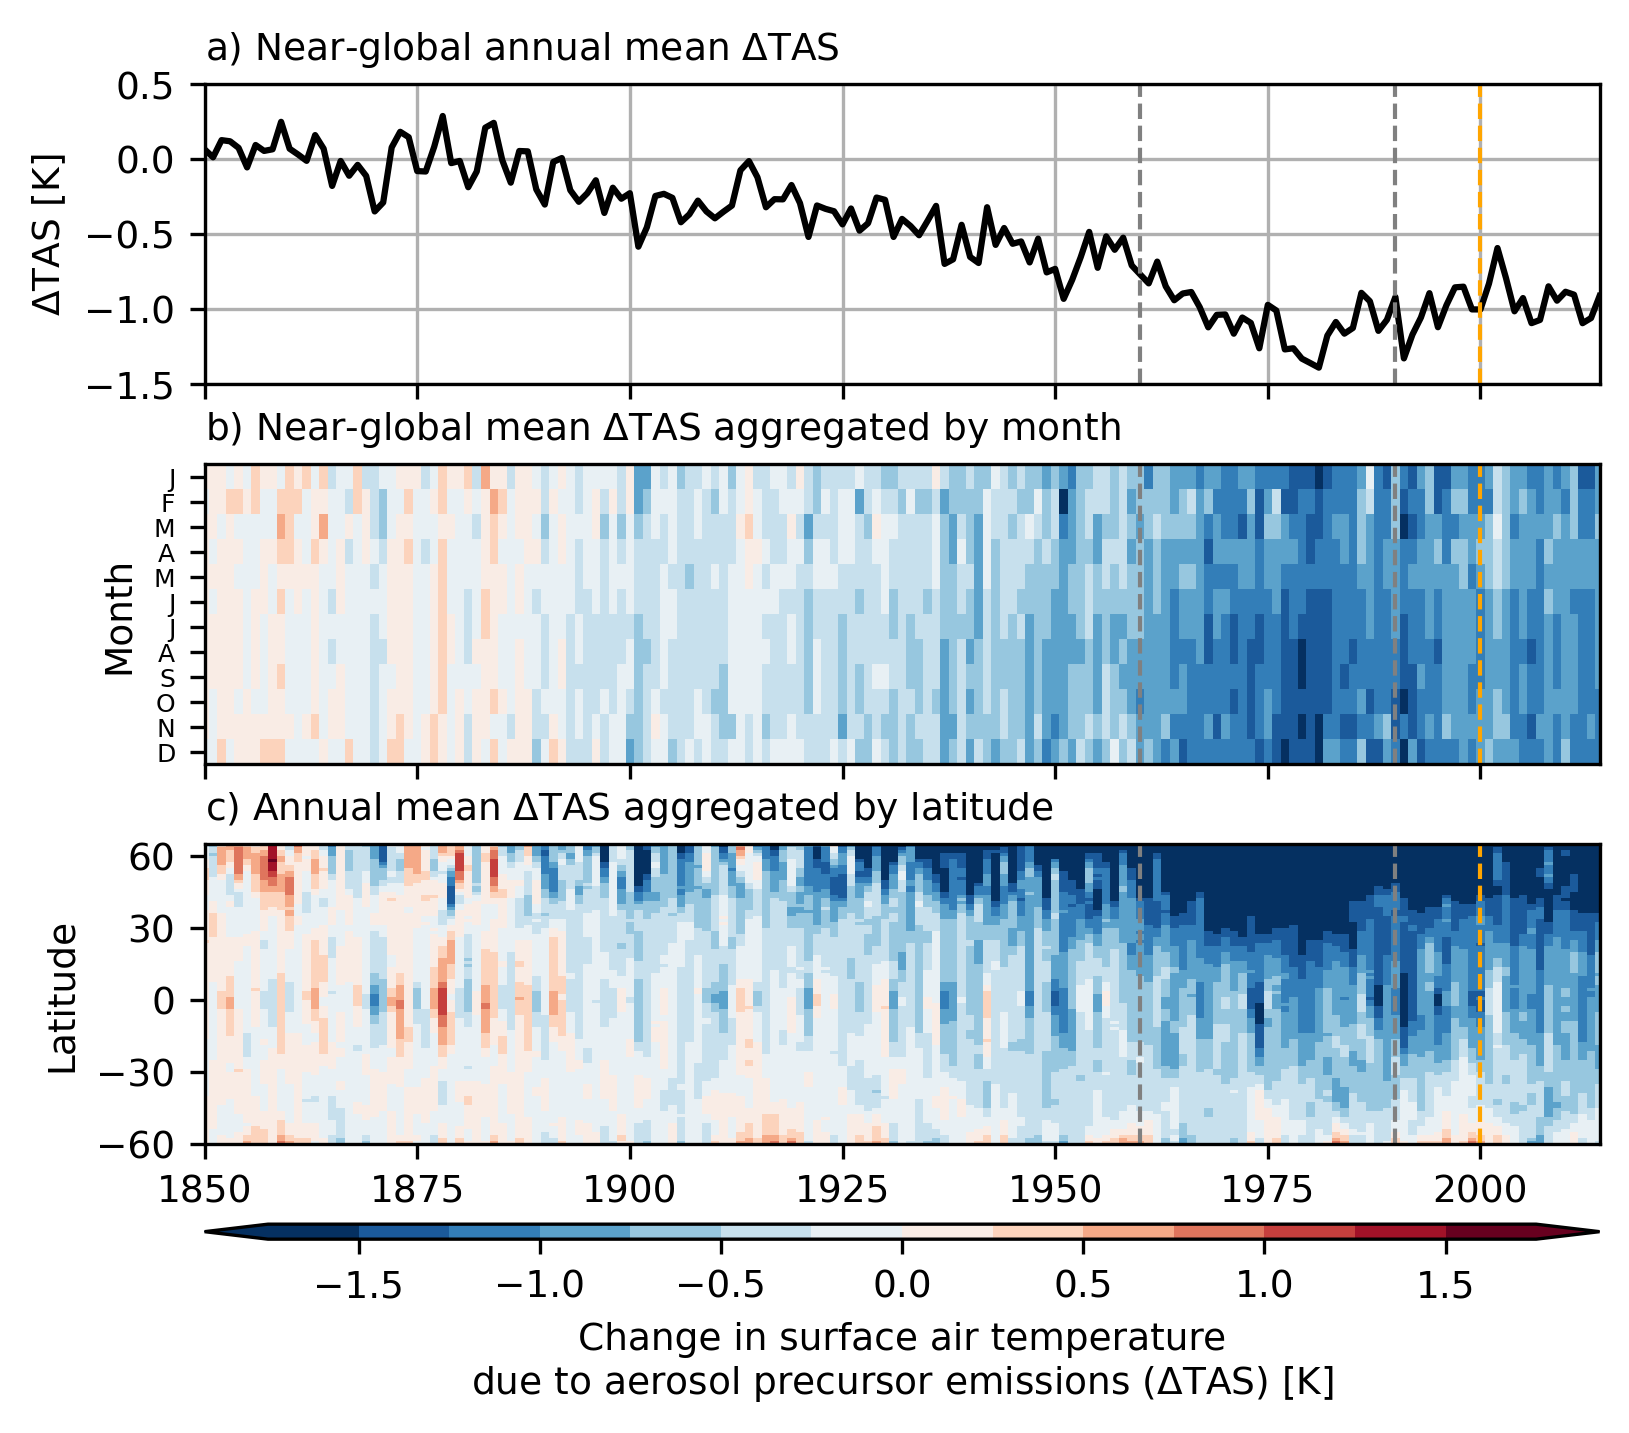
\includegraphics{Chapter4/Figs/tas_change_aerosols.png}
    \caption[Surface air temperature changes due to aerosol precursor emissions]{a) Annual mean surface air temperature changes due to aerosol precursor emissions averaged over latitude 60\textdegree S and 65\textdegree calculated from the difference between \hist{} and \histpiaer{}. b) Near-global mean surface air temperature aggregated by month and year. c) Near-global mean surface air temperature aggregated by month and latitude.}
    \label{fig:ch4:tas-change-aerosol}
\end{figure}


Aerosol not only modifies the surface temperature anomaly but also impacts historical trends and local temperature. Figure \ref{fig:ch4:tas-change-aerosol} shows the change in near-global mean TAS due to aerosol precursor emissions aggregated by month and latitude in subfigures b and c, respectively. Aerosol cooling is the strongest in the northern latitudes, collocating with the aerosol precursor emissions. At the maximum in the 1980s, aerosols cool down TAS by 1.5 K globally and more than 2 K in the northern hemisphere. After the pothole period, $\Delta$TAS slightly increases, and the Northern Hemisphere is not as cooled by aerosol. Near-global mean $\Delta$TAS aggregated by month show that during the pothole period, there is an increase in aerosol cooling from July up to November.


\begin{figure}
    \centering
    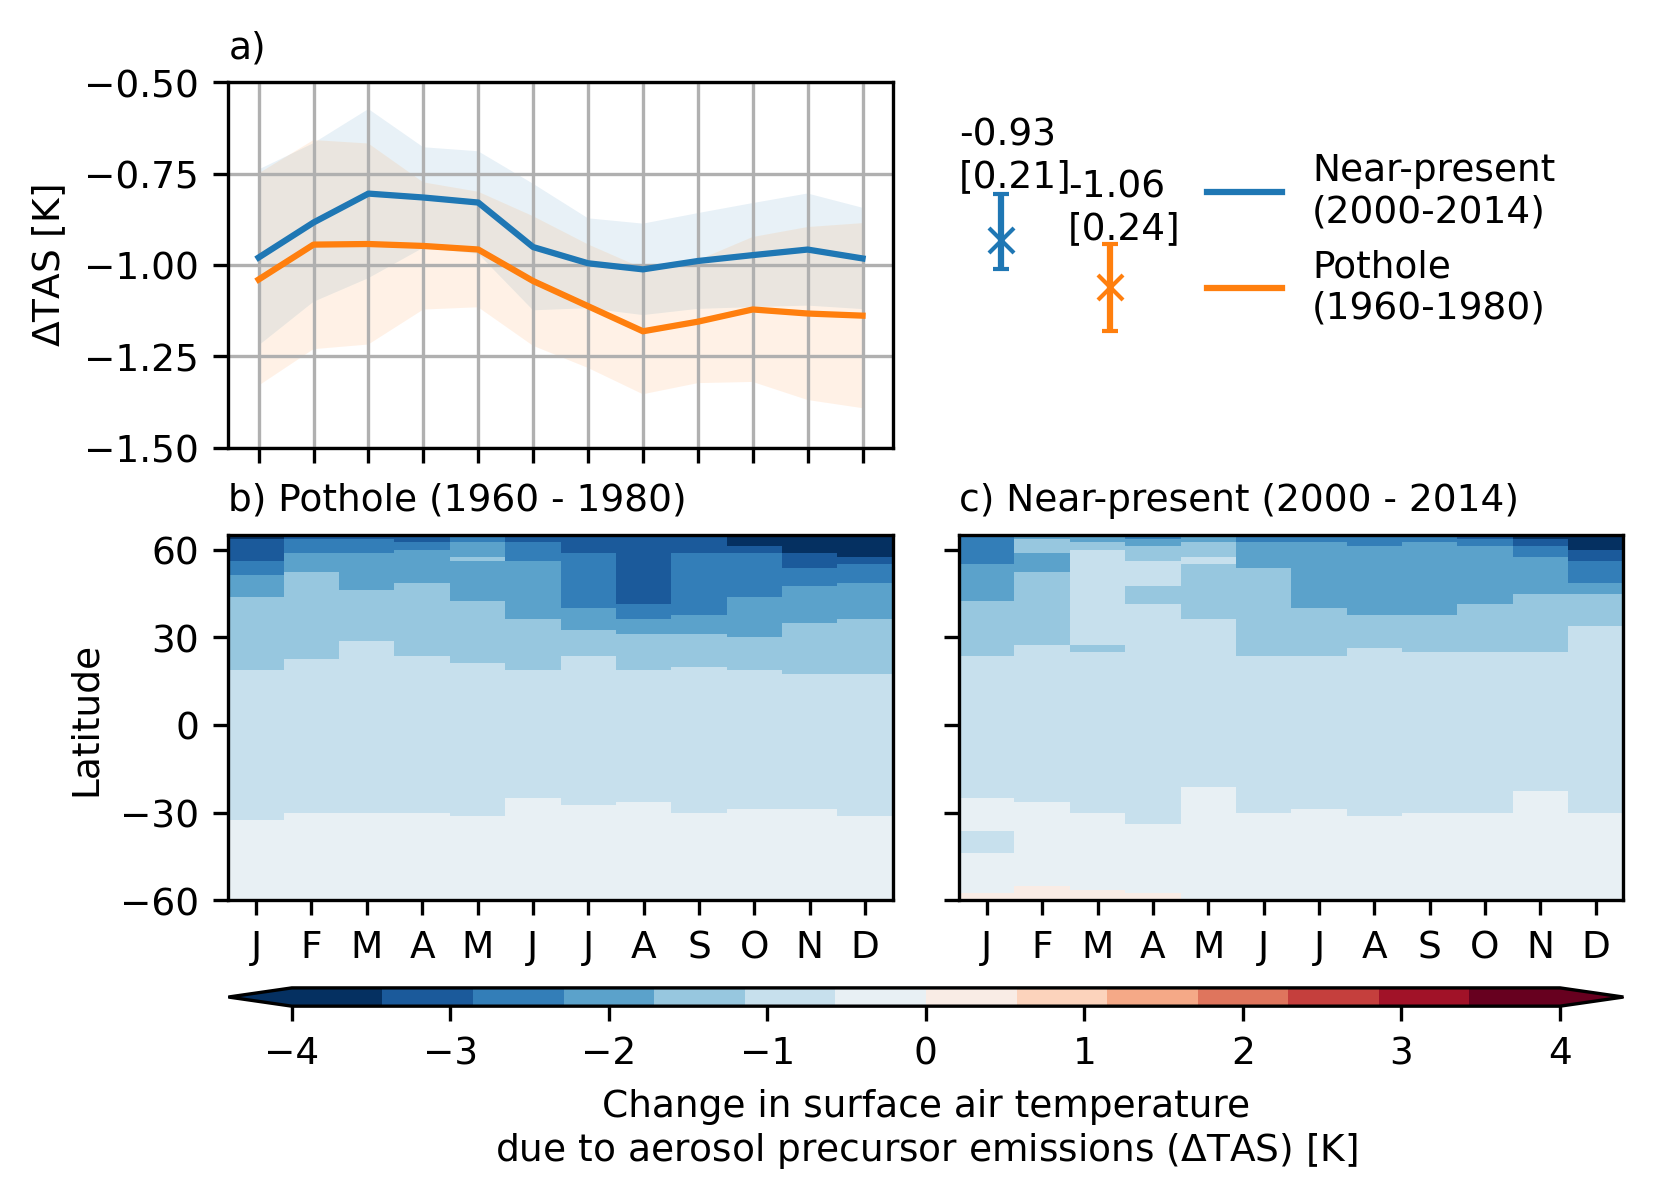
\includegraphics{Chapter4/Figs/tas_range.png}
    \caption[Change in surface air temperature due to aerosol precursor emissions for 1960--1989 and 2000-2014]{a) Near-global mean surface air temperature change due to aerosol precursor emissions (\hist{} minus \histpiaer{}) for the pothole and near-present period averaged over latitude 60\textdegree S and 65\textdegree N aggregated by month. $\Delta$TAS during b) pothole and c) near-present period aggregated by month and latitude. The notation next to a) shows the annual mean $\Delta$TAS and the range (maximum minus minimum) in square brackets.}
    \label{fig:ch4:tas-range}
\end{figure}


To quantify whether there is an abnormal summer cooling during the pothole period in the model, the $\Delta$TAS during the pothole period and the near-present are compared. Figure \ref{fig:ch4:tas-range} shows the difference of $\Delta$TAS between the maximum and minimum between two periods of interest: the pothole period (1960--1989) and near present (2000--2014). These are the difference between the \hist{} and the \histpiaer{} simulations. It shows the seasonal temperature changes due to aerosols, the global annual mean cooling, and the range (maximum minus minimum) of cooling during the year. Seasonal variations during both periods are similar, with aerosols exerting their cooling effects most significantly in August in the Northern Hemisphere, decreasing global surface air temperature by 1.21 K during the pothole period and 1 K in the near-present. The gap between the maximum and minimum $\Delta$TAS is greater during the pothole period (0.24 K compared to 0.21 K). Hence, aerosol precursor emissions contribute slightly more cooling, especially in summer during the pothole period, compared to the near present when the model does not underpredict TAS. However, it has to be noted that this difference is mild, and lower cooling in the near present may have been caused by higher BC emissions, which absorb radiation and lead to warming.

\section{Conclusions}


% points: oxidants, oxidation, the importance of cloud fraction,  lifetime, cloud, ERF, specific ERF, the correlation between SO2_OH and ERF, TAS
This chapter has quantitatively analysed the seasonal variation of \ce{SO2} oxidation and its impact on aerosol and cloud formation, radiative effects and surface air temperature. Due to more photochemical production of oxidants in summer, UKESM1 simulated more aerosol particles in summer and showed more negative ERF. Assuming that ERF due to aerosol is mainly contributed by sulfate, ERF per unit of \ce{SO2} emissions is reported, showing that \ce{SO2} has 2--4 times more potential to increase ERF when emitted in summer. The model also indicated slightly more aerosol cooling during the pothole period than in the present day. While a study by \citet{zhangRoleAnthropogenicAerosols2021} showed that sulfate loading correlates with pothole cooling temperature, we suggest that aerosol loading in summer may contribute more significantly to anomalous cooling. 


The seasonal variation in the radiative impact of sulfate aerosol may also have emission policy implications. \citet{bellouinRegionalSeasonalRadiative2016} suggested that more \ce{SO2} could be emitted in winter due to lesser climatic impact and could lead to a controlled emission policy. However, this chapter would suggest otherwise. Results in this chapter have shown that \ce{SO2} has a longer lifetime in winter, and the concentration could build up due to the decreased loss. Hence, \ce{SO2} is more likely to cause health impacts, and this angle of argument should be considered.


The recent UKESM1 model development may alter the results of this chapter. \citet{hardacreEvaluationSO2SO422021} evaluated the simulated surface \ce{SO2} and sulfate concentrations against ground-based measurement networks in the USA and Europe. In polluted areas, UKESM1 overpredicted surface \ce{SO2} by a factor of 3 while underpredicting surface sulfate by 25--35\%. The mean surface \ce{SO2} concentration was overestimated, especially in summer for the 33 Eastern American ground observation sites for the period 1987--2014 \citep{hardacreEvaluationSO2SO422021}. The updated UKESM1 with modified \ce{SO2} dry deposition scheme, called UKESM1.1, simulated a lower surface \ce{SO2} concentration but exacerbated the underprediction of sulfate \citep{mulcahyUKESM11DevelopmentEvaluation2023}. This pointed towards the possibility that a) the model might need further compensation for the sulfur cycle and an increase in chemical oxidation of \ce{SO2} to convert \ce{SO2} in sulfate and b) potentially too large dry deposition \citep{mulcahyUKESM11DevelopmentEvaluation2023}.


In the future, other ESMs may benefit from a similar analysis in this chapter. This will help us understand the role of aerosol formation in the pothole problem prevalent in many CMIP6 ESMs. 
